\documentclass[11pt,a4paper,openany]{book}
% ---------------------------------------------------------------------------
% Preamble for the CC5513 lecture notes
% ---------------------------------------------------------------------------
\usepackage[T1]{fontenc}
\usepackage[utf8]{inputenc}
\usepackage{lmodern}
\usepackage[a4paper,textwidth=155mm,top=27mm,bottom=30mm,hmarginratio=1:1,headsep=9mm]{geometry}
\usepackage{microtype}
\usepackage{amsmath,amssymb,amsthm,mathtools,bm}
\usepackage{graphicx}
\usepackage{booktabs,tabularx,multirow,array}
\usepackage[dvipsnames]{xcolor}
\usepackage{tikz}
\usetikzlibrary{arrows.meta,calc,positioning,decorations.markings,shapes.geometric,fit,backgrounds}
\usepackage[ruled,vlined,linesnumbered]{algorithm2e}
\usepackage{listings}
\usepackage[most]{tcolorbox}
\usepackage{enumitem}
\usepackage[font=small,labelfont=bf,margin=4mm]{caption}
\usepackage{subcaption}
\usepackage[numbers,sort&compress]{natbib}
\usepackage{fancyhdr}
\usepackage[colorlinks=true,linkcolor=MidnightBlue,citecolor=OliveGreen,urlcolor=RoyalBlue]{hyperref}
\usepackage[capitalise,noabbrev]{cleveref}

\graphicspath{{figs/}}
\setlist{itemsep=2pt,topsep=4pt}
\setlength{\parskip}{2pt}
\renewcommand{\bibname}{References}

% ------------------------------------------------------------------ headers
\pagestyle{fancy}
\fancyhf{}
\fancyhead[LE]{\small\nouppercase{\leftmark}}
\fancyhead[RO]{\small\nouppercase{\rightmark}}
\fancyfoot[C]{\small\thepage}
\renewcommand{\headrulewidth}{0.3pt}
\fancypagestyle{plain}{\fancyhf{}\fancyfoot[C]{\small\thepage}\renewcommand{\headrulewidth}{0pt}}

% ------------------------------------------------------------------ theorems
\theoremstyle{plain}
\newtheorem{theorem}{Theorem}[chapter]
\newtheorem{proposition}[theorem]{Proposition}
\newtheorem{lemma}[theorem]{Lemma}
\newtheorem{corollary}[theorem]{Corollary}
\theoremstyle{definition}
\newtheorem{definition}[theorem]{Definition}
\newtheorem{exercise}{Exercise}[chapter]
\theoremstyle{remark}
\newtheorem{remark}[theorem]{Remark}

\tcbset{colback=white,boxrule=0.5pt,arc=1.5pt,left=4pt,right=4pt,top=3pt,bottom=3pt,
        fonttitle=\bfseries\small,breakable}
\newtcbtheorem[number within=chapter]{example}{Example}%
  {colframe=MidnightBlue!70,colbacktitle=MidnightBlue!8,coltitle=black,colback=MidnightBlue!2}{ex}
\newtcolorbox{notebook}[1]{colframe=OliveGreen!70,colback=OliveGreen!3,colbacktitle=OliveGreen!10,
  coltitle=black,title={Companion notebook: \texttt{#1}}}
\newtcolorbox{keypoints}{colframe=BrickRed!60,colback=BrickRed!2,colbacktitle=BrickRed!8,
  coltitle=black,title={Key points}}

% ------------------------------------------------------------------ algorithms
\SetAlgoSkip{medskip}
\SetKwInOut{Input}{Input}
\SetKwInOut{Output}{Output}
\SetAlFnt{\small}
\SetAlCapFnt{\small}
\crefname{algocf}{Algorithm}{Algorithms}
\Crefname{algocf}{Algorithm}{Algorithms}
\crefname{example}{Example}{Examples}
\crefname{tcb@cnt@example}{Example}{Examples}
\crefname{exercise}{Exercise}{Exercises}

% ------------------------------------------------------------------ listings
\lstset{basicstyle=\ttfamily\footnotesize,keywordstyle=\color{MidnightBlue}\bfseries,
  commentstyle=\color{OliveGreen},stringstyle=\color{BrickRed},showstringspaces=false,
  frame=single,rulecolor=\color{black!25},breaklines=true,columns=fullflexible,
  language=Python,xleftmargin=2pt,xrightmargin=2pt,aboveskip=6pt,belowskip=4pt}

% ------------------------------------------------------------------ notation
\newcommand{\R}{\mathbb{R}}
\newcommand{\N}{\mathbb{N}}
\newcommand{\C}{\mathbb{C}}
\newcommand{\M}{\mathcal{M}}
\newcommand{\NN}{\mathcal{N}}
\newcommand{\bx}{\mathbf{x}}
\newcommand{\by}{\mathbf{y}}
\newcommand{\bz}{\mathbf{z}}
\newcommand{\bp}{\mathbf{p}}
\newcommand{\bq}{\mathbf{q}}
\newcommand{\bn}{\mathbf{n}}
\newcommand{\bu}{\mathbf{u}}
\newcommand{\bv}{\mathbf{v}}
\newcommand{\bc}{\mathbf{c}}
\newcommand{\bd}{\mathbf{d}}
\newcommand{\be}{\mathbf{e}}
\newcommand{\bt}{\mathbf{t}}
\newcommand{\bb}{\mathbf{b}}
\newcommand{\ba}{\mathbf{a}}
\newcommand{\br}{\mathbf{r}}
\newcommand{\bs}{\mathbf{s}}
\newcommand{\bo}{\mathbf{o}}
\newcommand{\bw}{\mathbf{w}}
\newcommand{\bfun}{\mathbf{f}}
\newcommand{\bg}{\mathbf{g}}
\newcommand{\bzero}{\mathbf{0}}
\newcommand{\mA}{\mathbf{A}}
\newcommand{\mB}{\mathbf{B}}
\newcommand{\mC}{\mathbf{C}}
\newcommand{\mD}{\mathbf{D}}
\newcommand{\mE}{\mathbf{E}}
\newcommand{\mG}{\mathbf{G}}
\newcommand{\mH}{\mathbf{H}}
\newcommand{\mI}{\mathbf{I}}
\newcommand{\mJ}{\mathbf{J}}
\newcommand{\mK}{\mathbf{K}}
\newcommand{\mL}{\mathbf{L}}
\newcommand{\mM}{\mathbf{M}}
\newcommand{\mP}{\mathbf{P}}
\newcommand{\mQ}{\mathbf{Q}}
\newcommand{\mR}{\mathbf{R}}
\newcommand{\mS}{\mathbf{S}}
\newcommand{\mT}{\mathbf{T}}
\newcommand{\mU}{\mathbf{U}}
\newcommand{\mV}{\mathbf{V}}
\newcommand{\mW}{\mathbf{W}}
\newcommand{\mX}{\mathbf{X}}
\newcommand{\mY}{\mathbf{Y}}
\newcommand{\mPhi}{\boldsymbol{\Phi}}
\newcommand{\mPsi}{\boldsymbol{\Psi}}
\newcommand{\mLambda}{\boldsymbol{\Lambda}}
\newcommand{\mPi}{\boldsymbol{\Pi}}
\newcommand{\mSigma}{\boldsymbol{\Sigma}}
\newcommand{\bdelta}{\boldsymbol{\delta}}
\newcommand{\bphi}{\boldsymbol{\phi}}
\newcommand{\Lap}{\Delta}
\newcommand{\T}{^{\mathsf{T}}}
\newcommand{\norm}[1]{\left\lVert #1\right\rVert}
\newcommand{\abs}[1]{\left\lvert #1\right\rvert}
\newcommand{\inner}[2]{\left\langle #1,#2\right\rangle}
\newcommand{\dd}{\,\mathrm{d}}
\DeclareMathOperator*{\argmin}{arg\,min}
\DeclareMathOperator*{\argmax}{arg\,max}
\DeclareMathOperator{\tr}{tr}
\DeclareMathOperator{\diag}{diag}
\DeclareMathOperator{\Div}{div}
\DeclareMathOperator{\area}{area}
\DeclareMathOperator{\vol}{vol}
\DeclareMathOperator{\sgn}{sgn}
\DeclareMathOperator{\rank}{rank}
\DeclareMathOperator{\atanh}{atanh}
\newcommand{\grad}{\nabla}

% figure helper: \fig[width]{file}{caption}{label}
\newcommand{\fig}[4][\textwidth]{%
  \begin{figure}[tbp]\centering\includegraphics[width=#1]{#2}\caption{#3}\label{#4}\end{figure}}
% figure at natural size
\newcommand{\fign}[3]{%
  \begin{figure}[tbp]\centering\includegraphics{#1}\caption{#2}\label{#3}\end{figure}}


\hypersetup{pdftitle={CC5513 Geometry Processing and Shape Analysis: Lecture Notes},
            pdfauthor={Compiled from the CC5513 course material (Universidad de Chile)}}

\begin{document}
\frontmatter

\begin{titlepage}
\centering
\vspace*{8mm}
{\large Universidad de Chile \\ Facultad de Ciencias F\'isicas y Matem\'aticas \\ Departamento de Ciencias de la Computaci\'on\par}
\vspace{16mm}
{\Huge\bfseries Geometry Processing\\[3mm] and Shape Analysis\par}
\vspace{8mm}
{\Large Lecture notes for CC5513\\ Procesamiento Geom\'etrico y An\'alisis de Formas\par}
\vspace{10mm}
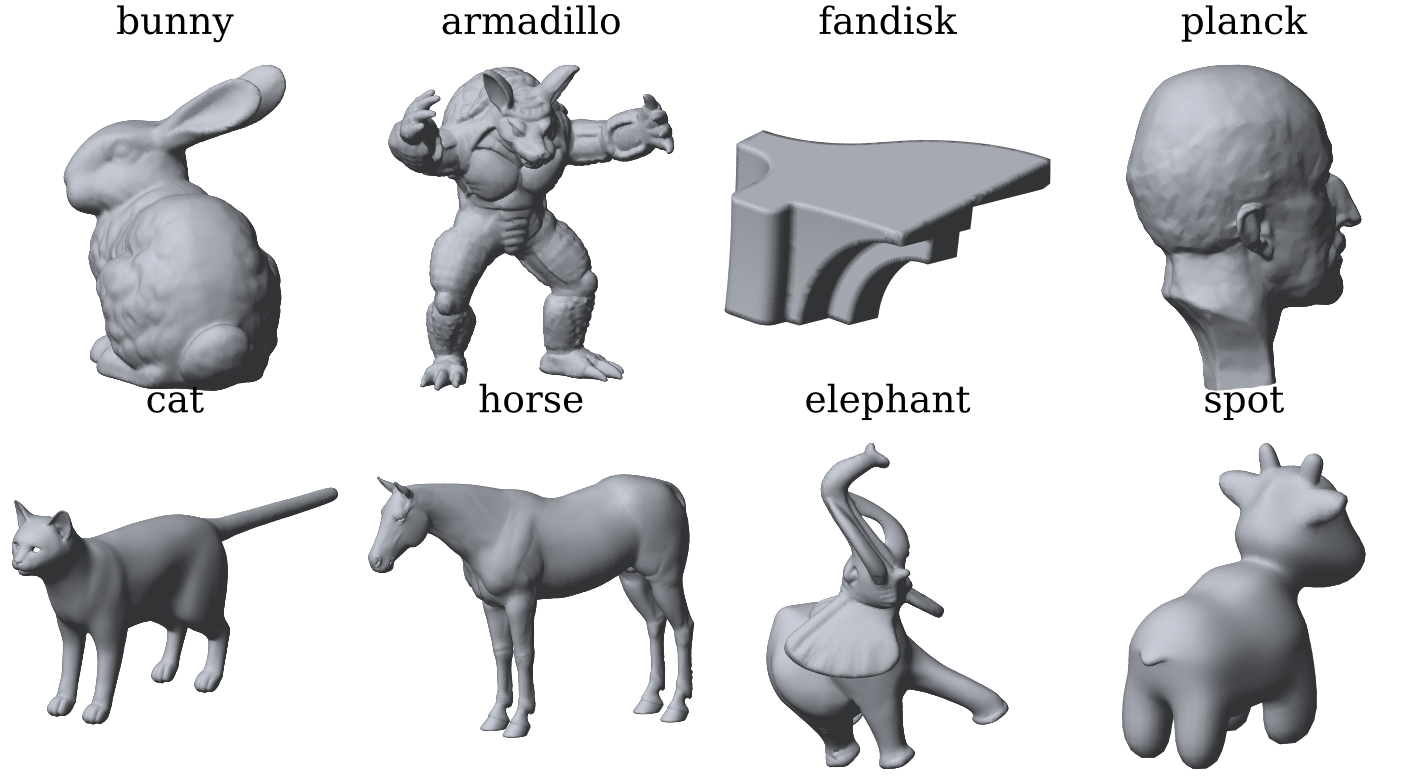
\includegraphics[width=0.78\textwidth]{ch01_gallery.png}\par
\vspace{8mm}
{\large A compendium of the fourteen course topics,\\ with worked examples, figures and reproducible code\par}
\vfill
{\normalsize Compiled from the course slides by Prof.~Ivan Sipiran and the companion notebooks.\\
All figures are generated by the scripts in \texttt{apuntes/scripts}.\par}
\vspace{6mm}
{\normalsize November 2026\par}
\end{titlepage}

\tableofcontents
\chapter*{Preface}
\addcontentsline{toc}{chapter}{Preface}
\markboth{Preface}{Preface}

These notes collect, in one place, the material of the course CC5513 \emph{Procesamiento
Geom\'etrico y An\'alisis de Formas} (geometry processing and shape analysis) taught at the
Departamento de Ciencias de la Computaci\'on of the Universidad de Chile. They follow the fourteen
slide decks of the course (\texttt{Slides/Tema1} to \texttt{Slides/Tema14}) and the six companion
notebooks, and they expand each topic with derivations, worked examples and figures. Every figure
was computed for these notes by a Python script in \texttt{apuntes/scripts}, mostly on the meshes
that ship with the course repository (\texttt{modelos/}) and with the demo packages in
\texttt{codigo/}; \cref{app:code} explains how to regenerate them.

\section*{How the notes map to the course}

\begin{center}
\footnotesize
\begin{tabular}{@{}rlll@{}}
\toprule
Chapter & Topic & Slides & Notebook \\
\midrule
\ref{ch:intro} & Introduction and pipeline & Tema 1 & \\
\ref{ch:repr} & 3D representations & Tema 2 & \texttt{Tema02\_Representaciones\_3D} \\
\ref{ch:ds} & Mesh data structures & Tema 3 & \\
\ref{ch:diffgeo} & Differential geometry & Tema 4 & \texttt{Tema04\_LaplaceBeltrami\_Suavizado} \\
\ref{ch:smooth} & Laplace--Beltrami and smoothing & Tema 4 & \texttt{Tema04\_LaplaceBeltrami\_Suavizado} \\
\ref{ch:acq} & 3D acquisition & Tema 5 & \\
\ref{ch:icp} & Local registration (ICP) & Tema 5 & \\
\ref{ch:global} & Global registration & Tema 6 & \texttt{Tema06\_4PCS\_RANSAC} \\
\ref{ch:recon} & Normals and reconstruction & Tema 7 & \texttt{Tema07\_Normales\_y\_Reconstruccion} \\
\ref{ch:ops} & Simplification, subdivision & Tema 8 & \\
\ref{ch:param} & Parameterization & Tema 9 & \\
\ref{ch:remesh} & Remeshing & Tema 10 & \\
\ref{ch:deform} & Deformation & Tema 11 & \\
\ref{ch:shape} & Shape analysis & Tema 12 & \\
\ref{ch:spectral} & Spectral shape analysis & Tema 13 & \texttt{Tema13\_Analisis\_Espectral} \\
\ref{ch:fmaps} & Functional maps & Tema 14 & \texttt{Tema14\_Shape\_Matching\_Mapas\_Funcionales} \\
\bottomrule
\end{tabular}
\end{center}

\section*{Notation and conventions}

Scalars are italic ($a, \lambda$), vectors bold lower case ($\bx, \bn$) and matrices bold upper
case ($\mL, \mM$). A triangle mesh is written $\M=(V,E,F)$ with $n=\abs{V}$ vertices, positions
$\bx_i\in\R^3$ stacked as the rows of $\mX\in\R^{n\times 3}$. $\mathcal N(i)$ is the one-ring of
vertex $i$ (its adjacent vertices) and $d_i=\abs{\mathcal N(i)}$ its valence. A function sampled at
the vertices is a vector $\bfun\in\R^n$. The unit normal is $\bn$, the mean curvature
$H=\tfrac12(\kappa_1+\kappa_2)$ and the Gaussian curvature $K=\kappa_1\kappa_2$.

\paragraph{Laplacian sign convention.} Two conventions coexist in the literature and in the
course. In \cref{ch:diffgeo,ch:smooth,ch:deform} we use the analyst's Laplacian
$\Lap f=\Div\grad f$, which is negative semi-definite; its discretisation is
$\Lap\approx\mM^{-1}\mC$, where $\mC$ is the cotangent \emph{stiffness} matrix (negative
semi-definite, rows summing to zero) and $\mM$ the lumped mass matrix. With this sign,
$\Lap\bx=-2H\bn$, where $\bn$ is the outward normal and $H>0$ on a sphere, so the diffusion flow
$\partial_t\bx=\Lap\bx$ moves convex regions inwards.
In \cref{ch:spectral,ch:fmaps} we follow the spectral geometry literature and use the positive
operator $L=-\Div\grad$, discretised by $\mL=-\mC$; its eigenproblem is
$\mL\bphi=\lambda\mM\bphi$ with $0=\lambda_1\le\lambda_2\le\cdots$ and eigenvectors normalised
by $\mPhi\T\mM\mPhi=\mI$. Each chapter recalls which convention it uses.

\paragraph{Units.} Unless stated otherwise, the meshes are rescaled to unit bounding-box
diagonal (\cref{ch:repr,ch:diffgeo,ch:smooth,ch:icp,ch:global,ch:recon,ch:ops,ch:param,ch:remesh,ch:deform})
or to unit surface area (\cref{ch:spectral,ch:fmaps}), so errors and distances are relative.

\paragraph{Reading the figures.} Renderings are orthographic with Lambert shading; colour maps
encode a scalar field, with the colour range stated in the caption when it matters. Numbers
quoted in captions are the values printed by the generating script.


\mainmatter
\chapter{Introduction}\label{ch:intro}

Geometry processing studies algorithms that acquire, represent, transform and analyse the shape
of three-dimensional objects. Shape analysis is the part of the field that extracts meaning from
geometry: it measures how similar two shapes are, finds corresponding points on them, detects
symmetries or retrieves a model from a large collection. Both rest on the same toolbox: a
discrete representation of a surface (usually a triangle mesh or a point cloud), a discrete
version of differential geometry (normals, curvature, the Laplace--Beltrami operator), and
numerical linear algebra to turn geometric goals into sparse linear systems or eigenproblems.

\section{Geometry everywhere}

Digital 3D shapes are produced and consumed in many domains:
\begin{itemize}
  \item \textbf{Entertainment and design}: characters and environments for films and games are
  modelled, textured (\cref{ch:param}), simplified for real time rendering (\cref{ch:ops}) and
  animated by deformation and skinning (\cref{ch:deform}).
  \item \textbf{Engineering and manufacturing}: CAD models are converted to meshes for
  simulation and 3D printing; scanned parts are compared against their design by registration
  (\cref{ch:icp,ch:global}).
  \item \textbf{Medicine}: organs segmented from CT or MRI volumes are extracted as iso-surfaces
  (\cref{ch:recon}) and compared across patients through correspondences (\cref{ch:fmaps}).
  \item \textbf{Cultural heritage}: archaeological artefacts are digitised with laser or
  structured-light scanners (\cref{ch:acq}), reconstructed, restored by exploiting symmetry and
  retrieved from digital collections (\cref{ch:shape}).
  \item \textbf{Robotics, autonomous driving and AR/VR}: depth sensors deliver point clouds at
  video rate that must be registered, segmented into primitives and interpreted on line.
\end{itemize}

\section{The geometry processing pipeline}

\Cref{fig:pipeline} organises the course as a pipeline. A physical object is measured by a 3D
scanner, which produces several partial point clouds, each in the coordinate system of the
sensor. \emph{Registration} brings the scans into a common frame, first coarsely with feature-based
or RANSAC-type methods and then precisely with the iterative closest point algorithm.
\emph{Reconstruction} estimates normals and fits a watertight surface to the merged points. The
result is then \emph{processed}: noise is removed by smoothing, the number of elements is reduced
by simplification or increased by subdivision, the element quality is improved by remeshing, a
planar parameterization is computed for texturing, and the shape can be edited by deformation.
Finally, \emph{analysis} describes the shape with descriptors that are invariant to the
transformations we want to ignore (rigid motions, scale, articulated poses) and uses them for
retrieval, classification and correspondence.

\begin{figure}[tbp]
\centering
\begin{tikzpicture}[node distance=4mm and 5mm, every node/.style={font=\small},
  box/.style={draw, rounded corners=2pt, align=center, minimum height=11mm, text width=23mm, fill=#1},
  box/.default=white, ar/.style={-{Stealth[length=2.2mm]}, thick}]
\node[box=MidnightBlue!8] (acq) {Acquisition\\ \footnotesize Ch.~\ref{ch:acq}};
\node[box=MidnightBlue!8, right=of acq] (reg) {Registration\\ \footnotesize Ch.~\ref{ch:icp}, \ref{ch:global}};
\node[box=MidnightBlue!8, right=of reg] (rec) {Reconstruction\\ \footnotesize Ch.~\ref{ch:recon}};
\node[box=OliveGreen!10, right=of rec, text width=30mm, minimum height=24mm] (proc)
  {Processing\\ \footnotesize smoothing (\ref{ch:smooth})\\ simplification, subdivision (\ref{ch:ops})\\
   parameterization (\ref{ch:param})\\ remeshing (\ref{ch:remesh})\\ deformation (\ref{ch:deform})};
\node[box=BrickRed!8, below=9mm of rec, text width=52mm] (ana)
  {Analysis: descriptors, retrieval, symmetry (\ref{ch:shape}),\\ spectral analysis (\ref{ch:spectral}),
   correspondences (\ref{ch:fmaps})};
\node[box=black!4, below=9mm of acq, text width=40mm] (found)
  {Foundations: representations (\ref{ch:repr}), data structures (\ref{ch:ds}),
   differential geometry (\ref{ch:diffgeo})};
\draw[ar] (acq) -- node[above, font=\scriptsize]{scans} (reg);
\draw[ar] (reg) -- node[above, font=\scriptsize]{points} (rec);
\draw[ar] (rec) -- node[above, font=\scriptsize]{mesh} (proc);
\draw[ar] (proc.south) |- (ana.east);
\draw[ar, dashed] (found.east) -- (ana.west);
\end{tikzpicture}
\caption{The geometry processing pipeline followed by the course. Numbers refer to chapters.}
\label{fig:pipeline}
\end{figure}

\section{Discrete surfaces as signals}

A recurring idea, made explicit by \citet{Taubin1995,Taubin2000}, is to treat the vertex
positions of a mesh as a signal defined on the surface. In classical signal processing the
Fourier basis diagonalises the second derivative: $\frac{\dd^2}{\dd x^2}e^{\mathrm{i}\omega x}=
-\omega^2e^{\mathrm{i}\omega x}$, so low frequencies are the slowly varying functions with small
$\omega^2$. On a surface the role of the second derivative is played by the Laplace--Beltrami
operator, and its eigenfunctions form a \emph{manifold harmonic} basis \citep{Vallet2008}. Noise
lives in the high frequencies, so smoothing is low-pass filtering (\cref{ch:smooth}); the lowest
frequencies encode the global shape, are invariant to bending without stretching, and are the
basis of spectral descriptors and functional maps (\cref{ch:spectral,ch:fmaps}). This single
operator links half of the chapters of these notes.

\fig[0.95\textwidth]{ch01_gallery.png}{Models used throughout the notes: the Stanford bunny and
armadillo, the fandisk CAD part, the Max Planck bust, a cat and a horse from the TOSCA collection
(available in several poses in \texttt{modelos/}), an elephant and the cow ``Spot''.}{fig:gallery}

\section{Discrete versus smooth geometry}

Real objects are smooth (or piecewise smooth) surfaces, but a computer stores a finite sample.
Throughout the course we ask two questions about every discrete quantity: what is the smooth
quantity it approximates, and does the approximation converge when the mesh is refined? Some
constructions are exact in a precise sense, for example the angle defect satisfies a discrete
Gauss--Bonnet theorem for any triangle mesh (\cref{ch:diffgeo}). Others depend on the quality of
the triangulation, for example the cotangent Laplacian has negative weights on obtuse triangles,
which is one motivation for remeshing (\cref{ch:remesh}). A classical result of
\citet{Wardetzky2007} shows that no discrete Laplacian can have all the properties of the smooth
one at the same time (\cref{ch:spectral}), so every method embodies a compromise.

\section{Tools}

The examples are written in Python with \texttt{numpy} and \texttt{scipy} (dense and sparse
linear algebra, KD-trees, sparse eigensolvers) and \texttt{matplotlib}. Mesh input/output, ray
casting and some reference implementations come from Open3D \citep{Zhou2018}, PyMeshLab
\citep{Cignoni2008} and scikit-image. Other widely used libraries are libigl, CGAL, OpenMesh,
trimesh and Polyscope. The standard references for the course are the book by
\citet{Botsch2010} and the discrete differential geometry notes of \citet{Crane2018}; the
differential geometry background is in \citet{doCarmo1976}.

\section{Roadmap}

\Cref{ch:repr,ch:ds,ch:diffgeo} build the foundations: how surfaces are represented, how meshes
are stored and traversed, and how normals and curvature are computed on them.
\Cref{ch:smooth} introduces the Laplace--Beltrami operator through mesh smoothing.
\Cref{ch:acq,ch:icp,ch:global,ch:recon} follow the acquisition pipeline: scanners, local and
global registration, normal estimation and surface reconstruction.
\Cref{ch:ops,ch:param,ch:remesh,ch:deform} cover mesh processing operations. Finally,
\cref{ch:shape,ch:spectral,ch:fmaps} turn to shape analysis: global and local descriptors,
spectral analysis and shape matching with functional maps. Two appendices summarise the linear
algebra used throughout and index the code.

\begin{keypoints}
\begin{itemize}[leftmargin=*]
  \item The course follows a pipeline: acquisition, registration, reconstruction, processing and
  analysis.
  \item Discrete operators must approximate smooth ones; convergence and robustness to the mesh
  quality are recurring concerns.
  \item The Laplace--Beltrami operator plays the role of the second derivative and its
  eigenfunctions generalise the Fourier basis to surfaces.
\end{itemize}
\end{keypoints}

\chapter{Representations of 3D Shapes}\label{ch:repr}

A 3D shape can be stored in many ways, and the choice decides which operations are cheap. A
scanner produces points, a physician receives a voxel volume, a designer edits spline patches, a
GPU draws triangles, and many modern algorithms prefer a function whose zero level set is the
surface. This chapter reviews the main representations, their strengths and costs, and the
conversions between them (\cref{fig:repr}). The companion notebook builds each one in Python.

\fig{ch02_representations.png}{The same object (the Stanford bunny) in five representations: an
oriented point cloud, a coarse triangle mesh, an occupancy voxel grid, a slice of a signed
distance function $f$ (blue inside, red outside, black zero level) and the mesh extracted from
$\{f=0\}$ by marching cubes.}{fig:repr}

\section{A taxonomy}

Two distinctions organise the zoo of representations.
\begin{itemize}
  \item \textbf{Surface versus volume.} A boundary (surface) representation stores only the
  interface between inside and outside: point clouds, meshes, parametric patches. A volumetric
  representation describes the whole space: voxel grids, octrees, implicit functions.
  \item \textbf{Explicit versus implicit.} An explicit representation lists or generates points of
  the surface, for example a parameterization $\bx(u,v)$ or the vertices of a mesh. An implicit
  representation gives a test: $\bx$ is on the surface if $f(\bx)=0$. Explicit forms make sampling
  and rendering easy; implicit forms make inside/outside queries, Boolean operations and changes of
  topology easy.
\end{itemize}

\begin{table}[tbp]
\centering\small
\begin{tabularx}{\textwidth}{@{}lXXX@{}}
\toprule
Representation & Strengths & Weaknesses & Typical source \\
\midrule
Point cloud & raw sensor output; trivial to store and transform & no connectivity, no
inside/outside, needs neighbourhood search & scanners, photogrammetry \\
Voxel grid & regular, trivial Boolean operations, convolution & memory $O(n^3)$, blocky,
resolution bound & CT/MRI, simulation, 3D CNNs \\
Parametric patch & smooth, compact, exact derivatives & topology fixed by the patch layout,
trimming, stitching & CAD (NURBS) \\
Triangle mesh & universal, GPU friendly, arbitrary topology & piecewise linear, quality
dependent operators & modelling, reconstruction \\
Implicit (SDF) & inside/outside, Booleans, topology changes free & surface not explicit,
extraction needed & reconstruction, modelling, neural fields \\
\bottomrule
\end{tabularx}
\caption{Overview of the representations discussed in this chapter.}
\label{tab:repr}
\end{table}

\section{Point clouds}\label{sec:pointclouds}

A point cloud is a finite set $P=\{\bp_i\}_{i=1}^n\subset\R^3$, optionally with attributes per
point such as a normal $\bn_i$, a colour or a confidence. In code it is simply an $n\times 3$ array.
Point clouds are the natural output of 3D scanners (\cref{ch:acq}) and the input of registration
and reconstruction. They carry no connectivity, so every geometric operation starts with a
neighbourhood query.

\subsection{Sampling a mesh}

To produce a point cloud from a mesh with uniform density with respect to area, pick a triangle
with probability proportional to its area and then a uniform point inside it. If $r_1,r_2\sim
U(0,1)$, the point
\begin{equation}
\bp=(1-\sqrt{r_1})\,\bx_a+\sqrt{r_1}(1-r_2)\,\bx_b+\sqrt{r_1}\,r_2\,\bx_c
\label{eq:triangle-sampling}
\end{equation}
is uniformly distributed in the triangle $(\bx_a,\bx_b,\bx_c)$. The square root compensates for the
fact that the segment at ``height'' $s$ from vertex $a$ has length proportional to $s$: the
density of $s=\sqrt{r_1}$ is $2s$, which is exactly the length weight.

Uniform random samples cluster and leave gaps. \emph{Poisson-disk} (blue noise) sampling enforces a
minimum distance $r$ between samples, which gives an even coverage with the same number of points
(\cref{fig:sampling}); a simple implementation draws a dense uniform sample and eliminates every
point closer than $r$ to an accepted one \citep{Bridson2007}. \emph{Voxel downsampling} replaces
the points that fall in each cell of a grid by their average and is the standard way to thin a
dense scan.

\fig{ch02_sampling.png}{Uniform random sampling versus Poisson-disk sampling of the bunny with
3000 points each. The histogram of nearest-neighbour distances shows the difference: random
samples have many very close pairs, while the Poisson-disk sample has none below the radius
$r=0.0128$ (unit bounding-box diagonal).}{fig:sampling}

\subsection{Neighbourhood queries and kd-trees}

Normal estimation, ICP, outlier removal and reconstruction all ask for the $k$ nearest neighbours
of a point or for all points within a radius. Brute force costs $O(n)$ per query and $O(n^2)$ for
all points. A \emph{kd-tree} \citep{Bentley1975,Friedman1977} partitions space recursively with
axis-aligned planes:
\begin{enumerate}
  \item choose a splitting axis (cycling $x,y,z$, or the axis of largest spread);
  \item split at the median coordinate, so both children hold half of the points;
  \item recurse until a leaf holds at most a few points.
\end{enumerate}
Construction costs $O(n\log n)$ with linear-time median selection, and the tree has depth
$O(\log n)$. A \emph{range query} descends only into cells that intersect the query box or ball. A
\emph{nearest-neighbour query} descends to the leaf containing the query, records the best
distance $d^\star$, and on the way back visits the other child of a node only if the splitting
plane is closer than $d^\star$; for $k$ neighbours $d^\star$ is the distance to the current
$k$-th best, kept in a max-heap. In low dimension the expected cost is $O(\log n)$ per query
(\cref{fig:kdtree,fig:kdbench}); in high dimension the pruning test rarely succeeds and the search
degenerates to brute force, which is why \cref{ch:fmaps} uses dense matrix products for
nearest neighbours in 100-dimensional spectral spaces.

\fig{ch02_kdtree.png}{A 2D kd-tree. Left: the cells produced by recursive median splits. Centre:
a range query visits only the cells that intersect the query rectangle (highlighted). Right: a
$k$-nearest-neighbour query ($k=6$).}{fig:kdtree}

\fign{ch02_kdtree_bench.pdf}{Time per query of brute force (linear in $n$) and of a kd-tree
(nearly constant), and the build time divided by $n$ (growing like $\log n$), measured with
\texttt{scipy.spatial.cKDTree} on uniform points.}{fig:kdbench}

\section{Volumetric representations}

\subsection{Voxel grids}

A voxel grid divides a bounding box into $n^3$ cubic cells and stores a value per cell: a binary
occupancy, a density (CT scans), a signed distance, or a feature vector (3D convolutional
networks). The grid is trivially indexed, neighbours are implicit, and Boolean operations are
cell-wise logical operations. The price is memory: a $512^3$ grid of floats needs 512\,MB, while
the surface only intersects $O(n^2)$ cells. Coarse grids make the shape blocky
(\cref{fig:voxels}). A surface voxelization marks the cells that contain surface points; a solid
voxelization also fills the interior, for example by casting a ray along each grid column and
toggling inside/outside at every surface crossing (parity rule). The volume of a solid is then
approximated by the number of occupied cells times the cell volume.

\fig[0.8\textwidth]{ch02_voxel_resolution.png}{Surface voxelization of the bunny at resolutions
$n=12,24,48$. The occupied cells are $432$, $1832$ and $7437$, that is $25\%$, $13\%$ and $6.7\%$ of
the $n^3$ cells: the count grows like $n^2$ and the fraction decreases like $1/n$, which motivates
sparse and adaptive grids.}{fig:voxels}

\subsection{Adaptive grids}

Because the interesting cells concentrate near the surface, adaptive structures refine only
there. An \emph{octree} splits a cell into eight children when it contains surface; memory becomes
proportional to the surface area. OpenVDB \citep{Museth2013} uses a shallow tree with large
fan-out (for example $32^3$, $16^3$ and $8^3$ nodes) similar to a B+tree, giving fast random
access, sparse storage of a narrow band around the surface, and dynamic topology, and it is the
industry standard for level sets in visual effects.

\section{Surfaces and manifoldness}

\begin{definition}[2-manifold]
A surface $S\subset\R^3$ is a \emph{2-manifold} if every point has a neighbourhood homeomorphic to
an open disk. It is a 2-manifold with boundary if every point has a neighbourhood homeomorphic to
a disk or to a half-disk.
\end{definition}

For a triangle mesh, manifoldness reduces to two combinatorial conditions: every edge is shared by
one (boundary) or two (interior) triangles, and the triangles around every vertex form a single
fan, closed for interior vertices and open for boundary vertices (\cref{fig:nonmanifold}). A
surface is \emph{orientable} if a consistent normal direction can be chosen; for meshes this means
the faces can be ordered so that every interior edge is traversed in opposite directions by its two
faces. Most algorithms in these notes assume oriented 2-manifold meshes, and data structures such as
the half-edge (\cref{ch:ds}) cannot even represent non-manifold configurations.

\begin{figure}[tbp]
\centering
\begin{tikzpicture}[scale=1.0, every node/.style={font=\small}]
  % manifold interior vertex
  \begin{scope}
    \foreach \a in {0,60,...,300} {\draw[fill=MidnightBlue!10] (0,0) -- (\a:1) -- (\a+60:1) -- cycle;}
    \fill (0,0) circle (1.5pt);
    \node at (0,-1.35) {manifold vertex};
  \end{scope}
  % boundary vertex
  \begin{scope}[xshift=3cm]
    \foreach \a in {0,45,90,135} {\draw[fill=MidnightBlue!10] (0,0) -- (\a:1) -- (\a+45:1) -- cycle;}
    \fill (0,0) circle (1.5pt);
    \node at (0,-1.35) {boundary vertex};
  \end{scope}
  % non-manifold edge
  \begin{scope}[xshift=6.2cm]
    \draw[fill=BrickRed!12] (0,-0.9) -- (0,0.9) -- (-1.1,0) -- cycle;
    \draw[fill=BrickRed!12] (0,-0.9) -- (0,0.9) -- (1.1,0) -- cycle;
    \draw[fill=BrickRed!25] (0,-0.9) -- (0,0.9) -- (0.55,0.45) -- cycle;
    \draw[very thick, BrickRed] (0,-0.9) -- (0,0.9);
    \node at (0,-1.35) {edge with 3 faces};
  \end{scope}
  % non-manifold vertex (bow tie)
  \begin{scope}[xshift=9.4cm]
    \draw[fill=BrickRed!12] (0,0) -- (-1,0.7) -- (-1,-0.7) -- cycle;
    \draw[fill=BrickRed!12] (0,0) -- (1,0.7) -- (1,-0.7) -- cycle;
    \fill[BrickRed] (0,0) circle (2pt);
    \node at (0,-1.35) {vertex with two fans};
  \end{scope}
\end{tikzpicture}
\caption{Manifold and non-manifold configurations. Left: the neighbourhood of a manifold vertex is
a disk (interior) or half-disk (boundary). Right: an edge shared by three triangles and a vertex
whose triangles form two separate fans are non-manifold.}
\label{fig:nonmanifold}
\end{figure}

\section{Parametric surfaces}

A parametric surface is a map $\bx:\Omega\subset\R^2\to\R^3$, $(u,v)\mapsto\bx(u,v)$. Sampling is
immediate, and derivatives $\bx_u,\bx_v$ are available in closed form, so normals and curvatures
are exact (\cref{ch:diffgeo}). The difficulty is global: a single patch has the topology of its
domain, so a complex object needs many patches whose boundaries must be stitched with continuity
conditions.

\paragraph{B\'ezier curves and patches.} The Bernstein polynomials
$B_i^n(t)=\binom{n}{i}t^i(1-t)^{n-i}$ are non-negative and sum to one. A B\'ezier curve with
control points $\bc_0,\dots,\bc_n$ is $\bx(t)=\sum_i B_i^n(t)\bc_i$: it interpolates the end
points, is tangent to the control polygon there, and lies in its convex hull. The tensor-product
patch
\begin{equation}
\bx(u,v)=\sum_{i=0}^{m}\sum_{j=0}^{n}B_i^m(u)\,B_j^n(v)\,\bc_{ij}
\end{equation}
is controlled by a grid of points (\cref{fig:parametric}). \emph{B-splines} replace the global
Bernstein basis by piecewise polynomials with local support, so moving a control point changes the
surface only nearby, and \emph{NURBS} (non-uniform rational B-splines) add weights,
$\bx(u)=\sum_i w_iN_i(u)\bc_i/\sum_iw_iN_i(u)$, which allows exact conics such as circles. NURBS are
the standard of CAD; the slides of Tema 8 contrast them with triangle meshes: NURBS are compact and
smooth but need trimming curves and stitching for complex topology, whereas meshes handle
arbitrary topology uniformly.

\fig[0.95\textwidth]{ch02_parametric.png}{Left: a bicubic B\'ezier patch and its $4\times4$
control net; the patch interpolates the four corner control points. Right: a torus generated by
sampling $\bx(u,v)=((R+r\cos v)\cos u,(R+r\cos v)\sin u,r\sin v)$ on a periodic $(u,v)$ grid and
connecting neighbouring samples; the mesh has Euler characteristic $0$.}{fig:parametric}

\section{Triangle meshes}

A triangle mesh $\M=(V,E,F)$ consists of vertices with positions $\bx_i\in\R^3$ (the geometry) and
triangles given as triples of vertex indices (the connectivity or topology). It defines a
piecewise linear surface: every point of a triangle is a convex combination of its corners. The
approximation error of a smooth surface by a mesh with edge length $h$ is $O(h^2)$, so halving the
edges reduces the error by four at the cost of four times as many faces.

Triangles are preferred over general polygons because they are always planar, every polygon can
be triangulated, interpolation of attributes inside a triangle is linear and unambiguous
(barycentric coordinates), and graphics hardware is built around them.

\subsection{Euler's formula}

\begin{theorem}[Euler--Poincar\'e]
For a closed orientable polygonal mesh of genus $g$ (the number of handles),
\begin{equation}
V-E+F=\chi=2-2g .
\end{equation}
With $b$ boundary loops, $\chi=2-2g-b$.
\end{theorem}

For a closed triangle mesh each face has three edges and each edge two faces, so $2E=3F$.
Substituting into Euler's formula gives
\begin{equation}
E=3(V-\chi),\qquad F=2(V-\chi),
\end{equation}
so for large meshes $F\approx 2V$, $E\approx 3V$, and the average valence is $2E/V\approx 6$.
These ratios are useful to estimate memory (\cref{ch:ds}) and explain why regular meshes have
valence 6 (\cref{ch:remesh}).

\begin{example}{Counting elements}{euler}
\Cref{fig:euler} shows three closed meshes. The icosphere has $V=162$, $E=480$, $F=320$ and
$\chi=162-480+320=2$ (genus 0). The torus has $648-1944+1296=0$ (genus 1), and the double torus
$1498-4500+3000=-2$ (genus 2). In each case $2E=3F$ holds exactly, and $F=2(V-\chi)$:
for the double torus $2(1498+2)=3000$.
\end{example}

\fig[0.95\textwidth]{ch02_euler.png}{The Euler characteristic $\chi=V-E+F$ depends only on the
topology: $2$ for the sphere, $0$ for the torus and $-2$ for the double torus, whatever the
triangulation.}{fig:euler}

\section{Implicit surfaces}\label{sec:implicit}

An implicit surface is the zero level set $S=\{\bx: f(\bx)=0\}$ of a function $f:\R^3\to\R$, with
the convention $f<0$ inside and $f>0$ outside. If $\grad f\neq\bzero$ on $S$, the surface is a
smooth manifold and the outward normal is $\bn=\grad f/\norm{\grad f}$. A \emph{signed distance
function} (SDF) is the special case $\abs{f(\bx)}=\operatorname{dist}(\bx,S)$; it satisfies the
eikonal equation $\norm{\grad f}=1$ almost everywhere, and $f(\bx)$ tells how far one can move
from $\bx$ without hitting the surface (the basis of sphere tracing).

\paragraph{Primitives.} The SDF of a sphere of centre $\bc$ and radius $r$ is
$f(\bx)=\norm{\bx-\bc}-r$. For an axis-aligned box of half sizes $\bb$, with
$\bq=\abs{\bx}-\bb$ (component-wise),
$f(\bx)=\norm{\max(\bq,\bzero)}+\min(\max(q_x,q_y,q_z),0)$.

\paragraph{Constructive solid geometry.} Boolean operations become arithmetic on the functions:
\begin{equation}
A\cup B:\ \min(f_A,f_B),\qquad A\cap B:\ \max(f_A,f_B),\qquad A\setminus B:\ \max(f_A,-f_B).
\end{equation}
The results are not exact distances any more (they are bounds), but their zero sets are correct. A
\emph{smooth union} replaces the minimum by a smooth minimum, for example the polynomial
$\operatorname{smin}_k(a,b)=\min(a,b)-h^2k/4$ with $h=\max(k-\abs{a-b},0)/k$, which blends the
two shapes over a width $k$ (\cref{fig:csg}).

\fig{ch02_csg.png}{Constructive solid geometry with signed distance functions. The first four
panels show a slice of $f$ for the union, intersection, difference and smooth union of a disk and a
square (dotted outlines); the solid line is the zero level set. Right: a 3D solid built as (box
$\cap$ sphere) minus three cylinders and extracted with marching cubes.}{fig:csg}

Implicit surfaces handle topology changes for free (two blobs merge when their functions do), and
inside/outside tests are a sign evaluation. Their weakness is that the surface is not explicit:
rendering or measuring it requires either ray marching or extraction of a mesh with marching cubes
(\cref{sec:marching}). Surface reconstruction methods (\cref{ch:recon}) build an implicit function
from points precisely to exploit these advantages, and recent neural fields store $f$ as the
weights of a network.

\section{Converting between representations}

The notebook closes with a map of conversions, summarised here:
\begin{itemize}
  \item mesh $\to$ points: area-weighted sampling \eqref{eq:triangle-sampling} or the vertices;
  \item points $\to$ mesh: surface reconstruction (\cref{ch:recon});
  \item mesh or points $\to$ voxels: rasterisation, ray casting for solid voxelization;
  \item mesh $\to$ SDF: closest-point queries plus an inside/outside test (winding number or ray
  parity);
  \item SDF or voxels $\to$ mesh: marching cubes or marching tetrahedra (\cref{sec:marching});
  \item parametric $\to$ mesh: sample a $(u,v)$ grid and connect neighbours (\cref{fig:parametric}).
\end{itemize}
Every conversion loses something: sampling loses connectivity, voxelization loses detail below the
cell size, and meshing an SDF loses sharp features unless special care is taken.

\begin{notebook}{Tema02\_Representaciones\_3D.ipynb}
Builds a point cloud from a mesh, downsamples it with a voxel grid, estimates normals and queries a
KD-tree; writes a mesh by hand and inspects normals and valences; voxelizes surfaces and solids
(ray casting) and computes volume by counting voxels; models with SDFs and Boolean operations and
extracts meshes with marching cubes; builds a torus from a parametric grid and checks Euler's
formula.
\end{notebook}

\begin{keypoints}
\begin{itemize}[leftmargin=*]
  \item Explicit representations make sampling easy; implicit ones make inside/outside, Booleans and
  topology changes easy.
  \item Point clouds need neighbourhood structures; kd-trees give $O(\log n)$ queries in 3D.
  \item Dense voxel grids cost $O(n^3)$ memory; sparse hierarchies (octrees, OpenVDB) store only the
  narrow band near the surface.
  \item For closed triangle meshes $V-E+F=2-2g$, $F\approx2V$, $E\approx3V$ and the mean valence is
  close to 6.
\end{itemize}
\end{keypoints}

\section*{Exercises}
\begin{exercise}
Prove that \eqref{eq:triangle-sampling} gives a uniform distribution on the triangle. Hint: compute
the Jacobian of the map $(r_1,r_2)\mapsto\bp$.
\end{exercise}
\begin{exercise}
A closed triangle mesh of genus 3 has $10\,000$ vertices. How many edges and faces does it have?
\end{exercise}
\begin{exercise}
Write the SDF of a capsule (the set of points within distance $r$ of a segment $[\ba,\bb]$) and of
a torus with radii $R>r$ centred at the origin with axis $z$.
\end{exercise}
\begin{exercise}
Estimate the memory of a dense $1024^3$ occupancy grid stored with one bit per voxel and of an
octree that stores only the leaves intersecting a surface of area $A$ at the same resolution.
\end{exercise}

\chapter{Mesh Data Structures}\label{ch:ds}

The algorithms of the following chapters do not only read vertex positions: they walk around
vertices, visit the neighbours of a face, find boundary loops, and modify the connectivity by
splitting, collapsing and flipping edges. The data structure that stores a mesh determines how
fast these operations are and how much memory they need. This chapter compares the classical
choices, from the simplest list of triangles to the half-edge structure used by most geometry
processing libraries.

\section{Requirements}

A mesh data structure must answer three kinds of requests efficiently:
\begin{enumerate}
  \item \textbf{Rendering and geometric queries}: positions of the vertices of a face, normals,
  areas, bounding boxes.
  \item \textbf{Adjacency queries}: the vertices, edges and faces incident to a vertex (its
  \emph{one-ring}), the faces adjacent to a face, the two faces of an edge, whether an element lies
  on the boundary.
  \item \textbf{Modifications}: inserting and deleting elements, splitting faces and edges,
  collapsing edges and flipping them (\cref{ch:ops,ch:remesh}).
\end{enumerate}
We measure memory per vertex using the ratios of \cref{ch:repr}: $F\approx 2V$ and $E\approx 3V$,
4 bytes per index and 12 bytes per position (three single-precision floats).

\section{Face-based structures}

\paragraph{Face set.} The simplest structure stores, for each triangle, the three positions of its
corners. This is the STL format used by 3D printers. It needs $3\times12=36$ bytes per face, that
is $72$ bytes per vertex, and it stores every position about six times. There is no explicit
connectivity: two triangles are neighbours only if they happen to share coordinates, so
adjacency queries require comparing floating-point positions, which is slow and fragile.

\paragraph{Indexed face set.} Vertices are stored once in an array and each face stores three
indices into it. This is the structure of the OBJ, OFF and PLY formats and of most rendering APIs
(vertex and index buffers). Memory is $12$ bytes per vertex plus $12$ bytes per face, about $36$
bytes per vertex. For example, a tetrahedron in OFF format is
\begin{lstlisting}[language={},numbers=none]
OFF
4 4 0
0 0 0
1 0 0
0 1 0
0 0 1
3 0 2 1
3 0 1 3
3 0 3 2
3 1 2 3
\end{lstlisting}
where each face lists its vertices counter-clockwise when seen from outside, so the normal
$(\bx_b-\bx_a)\times(\bx_c-\bx_a)$ points outwards. The indexed face set shares vertices, which
makes the mesh topologically meaningful, but adjacency queries remain expensive: finding the faces
around a vertex requires scanning all faces, $O(F)$ per query.

\paragraph{Face-based connectivity.} Adding references makes local queries constant time. Each
face stores its three vertices and its three neighbouring faces, and each vertex stores one
incident face. This needs $16$ bytes per vertex and $24$ bytes per face, about $64$ bytes per
vertex. Walking around a vertex is possible (from a face, move to the neighbour that shares the
vertex) but requires case distinctions to know which of the three neighbours to take, and the
structure only supports triangles (or a fixed polygon size).

\section{Edge-based structures}

\paragraph{Winged edge.} The winged-edge structure of \citet{Baumgart1975} is built around
edges. Each edge stores its two vertices, its two faces, and the previous and next edges in each of
the two faces (the four ``wings''): 8 references, 32 bytes. Each vertex and face stores one
incident edge. Memory is about $120$ bytes per vertex, and since an edge has no intrinsic
orientation, every traversal step must test in which of the two faces it is moving.

\paragraph{Half-edge.} The half-edge structure \citep{Mantyla1988,Kettner1999} removes the
orientation ambiguity by splitting each edge into two directed \emph{half-edges} with opposite
directions. Each half-edge belongs to exactly one face, which it traverses counter-clockwise, and
stores (\cref{fig:halfedge}):
\begin{itemize}
  \item the vertex it points to, $\operatorname{to}(h)$;
  \item its opposite half-edge, $\operatorname{opp}(h)$;
  \item the next half-edge in its face, $\operatorname{next}(h)$ (optionally also
  $\operatorname{prev}(h)$);
  \item its face, $\operatorname{face}(h)$, or a null value for boundary half-edges.
\end{itemize}
Each vertex stores one outgoing half-edge and each face one of its half-edges. With $6V$
half-edges of 16 bytes (20 with $\operatorname{prev}$), memory is about $120$ to $144$ bytes per
vertex. All adjacency queries become short loops without case distinctions, the structure handles
arbitrary polygons, and boundaries are represented by half-edges without a face.

\begin{figure}[tbp]
\centering
\begin{tikzpicture}[scale=1.25, every node/.style={font=\small},
  he/.style={-{Stealth[length=2.2mm]}, thick}, op/.style={-{Stealth[length=2.2mm]}, thick, BrickRed}]
  \coordinate (A) at (0,0); \coordinate (B) at (3,0); \coordinate (C) at (1.5,2.1); \coordinate (D) at (1.5,-2.1);
  \fill[MidnightBlue!6] (A) -- (B) -- (C) -- cycle;
  \fill[black!4] (A) -- (D) -- (B) -- cycle;
  \draw (A) -- (B) -- (C) -- cycle; \draw (A) -- (D) -- (B);
  \foreach \p in {A,B,C,D} \fill (\p) circle (1.6pt);
  % half-edges of the upper face (counter-clockwise)
  \draw[he, MidnightBlue] ($(A)!0.12!(B)+(0,0.1)$) -- ($(A)!0.88!(B)+(0,0.1)$) node[midway, above] {$h$};
  \draw[he] ($(B)!0.14!(C)+(-0.09,-0.03)$) -- ($(B)!0.86!(C)+(-0.09,-0.03)$) node[midway, right=2pt] {$\operatorname{next}(h)$};
  \draw[he] ($(C)!0.14!(A)+(0.09,-0.03)$) -- ($(C)!0.86!(A)+(0.09,-0.03)$) node[midway, left=2pt] {$\operatorname{prev}(h)$};
  \draw[op] ($(B)!0.12!(A)+(0,-0.1)$) -- ($(B)!0.88!(A)+(0,-0.1)$) node[midway, below] {$\operatorname{opp}(h)$};
  \node at (1.5,0.75) {$\operatorname{face}(h)$};
  \node[below left] at (A) {$\operatorname{from}(h)$};
  \node[below right] at (B) {$\operatorname{to}(h)$};
\end{tikzpicture}
\caption{The half-edge $h$ goes from vertex $\operatorname{from}(h)$ to $\operatorname{to}(h)$ and
belongs to the face on its left. Its successor and predecessor in that face are
$\operatorname{next}(h)$ and $\operatorname{prev}(h)$; the half-edge running in the opposite
direction, in the neighbouring face, is $\operatorname{opp}(h)$.}
\label{fig:halfedge}
\end{figure}

\subsection{Traversals}

The defining operation of the half-edge structure is the circulation around a vertex. Starting
from an outgoing half-edge $h$ of vertex $v$, the next outgoing half-edge in counter-clockwise
order is $\operatorname{opp}(\operatorname{prev}(h))$, and in clockwise order
$\operatorname{next}(\operatorname{opp}(h))$. \Cref{alg:onering} lists the one-ring; the same loop
gives the incident faces ($\operatorname{face}(h)$) and the valence (number of iterations).

\begin{algorithm}[tbp]
\caption{One-ring of a vertex in a half-edge mesh.}\label{alg:onering}
\Input{vertex $v$ with outgoing half-edge $h_0=\operatorname{out}(v)$}
\Output{list $R$ of neighbouring vertices in counter-clockwise order}
$R\gets[\,]$; $h\gets h_0$\;
\Repeat{$h=h_0$}{
  append $\operatorname{to}(h)$ to $R$\;
  $h\gets\operatorname{opp}(\operatorname{prev}(h))$\tcp*{rotate to the next outgoing half-edge}
}
\end{algorithm}

Other queries are equally local. The two faces of an edge are $\operatorname{face}(h)$ and
$\operatorname{face}(\operatorname{opp}(h))$; the vertices of a face are obtained by following
$\operatorname{next}$ until returning to the start; a vertex is on the boundary if one of its
outgoing half-edges has no face, and conventionally $\operatorname{out}(v)$ is chosen to be that
half-edge, so the test is $O(1)$; boundary loops are traced by following $\operatorname{next}$
among boundary half-edges.

\fig[0.95\textwidth]{ch03_halfedge_valence.png}{Left: circulation around a vertex with the
rule $h\leftarrow\operatorname{opp}(\operatorname{prev}(h))$; the numbers give the visiting order of
the outgoing half-edges. Right: valence histograms of the bunny (mean $5.99$) and the armadillo
(mean $6.00$), as predicted by Euler's formula.}{fig:valence}

\subsection{Building a half-edge mesh from an indexed face set}

\begin{enumerate}
  \item For every face $(a,b,c)$ create the half-edges $a\to b$, $b\to c$, $c\to a$ with their
  $\operatorname{next}$ links and face, and insert each one in a hash map keyed by the ordered pair
  $(\text{from},\text{to})$.
  \item For every half-edge $i\to j$, look up $(j,i)$; if found, link them as opposites.
  \item Half-edges without opposite are on the boundary: create the missing boundary half-edges
  (without face) and link them into boundary loops.
  \item If a key $(i,j)$ appears twice, two faces traverse the same edge in the same direction: the
  mesh is either inconsistently oriented or non-manifold, and must be repaired first.
\end{enumerate}
The construction is $O(F)$ expected time. The same pairing step is how orientation consistency is
checked in practice.

\begin{example}{Two triangles}{twotri}
Take faces $f_0=(0,1,2)$ and $f_1=(0,2,3)$, a square split along the diagonal $0$--$2$. The
half-edges of $f_0$ are $h_0:0\to1$, $h_1:1\to2$, $h_2:2\to0$ and those of $f_1$ are $h_3:0\to2$,
$h_4:2\to3$, $h_5:3\to0$. The only pair of opposite keys is $(2,0)$ and $(0,2)$, so
$\operatorname{opp}(h_2)=h_3$. The other four half-edges are on the boundary and get boundary
partners. Circulating around vertex $0$ from $h_0$: $\operatorname{prev}(h_0)=h_2$, so the next
outgoing half-edge is $\operatorname{opp}(h_2)=h_3$; then $\operatorname{prev}(h_3)=h_5$, whose
opposite is the boundary half-edge $0\to3$, which closes the loop. The one-ring of $0$ is
$(1,2,3)$, in counter-clockwise order.
\end{example}

\section{Index-based structures for triangle meshes}

For pure triangle meshes the half-edges can be numbered implicitly, so that most pointers are
computed instead of stored.

\paragraph{Directed edges.} \citet{Campagna1998} number the half-edges of face $f$ as $3f$,
$3f+1$, $3f+2$. Then
\begin{equation}
\operatorname{face}(h)=\lfloor h/3\rfloor,\qquad
\operatorname{next}(h)=3\lfloor h/3\rfloor+(h+1)\bmod 3,\qquad
\operatorname{prev}(h)=3\lfloor h/3\rfloor+(h+2)\bmod 3,
\end{equation}
and only $\operatorname{to}(h)$ (which is the face's index array) and $\operatorname{opp}(h)$ are
stored. Memory drops to about $64$ bytes per vertex while keeping all half-edge traversals.

\paragraph{Corner table.} \citet{Rossignac2001} use the same idea with \emph{corners}: corner
$c=3f+i$ is the $i$-th corner of face $f$, $V[c]$ is its vertex and $O[c]$ the opposite corner
across the edge facing $c$. The next and previous corners are computed arithmetically. The corner
table was designed for mesh compression (Edgebreaker) and is used by GPU-friendly libraries.

\paragraph{Beyond manifold surfaces.} Half-edges cannot represent an edge with three faces or a
vertex with two fans. Non-manifold models (for example CAD assemblies or meshes produced by
Boolean operations) need dedicated structures \citep{DeFloriani2003}, or a preprocessing step that
splits non-manifold vertices and edges. Compact array-based variants of the half-edge idea also exist
for volumetric meshes \citep{Lage2005}.

\begin{table}[tbp]
\centering\small
\begin{tabular}{@{}lccc@{}}
\toprule
Structure & Bytes per vertex & One-ring query & Arbitrary polygons \\
\midrule
Face set (STL) & 72 & no connectivity & yes \\
Indexed face set (OBJ/OFF) & 36 & $O(F)$ & yes \\
Face-based connectivity & 64 & $O(1)$, case analysis & no \\
Winged edge & 120 & $O(1)$, case analysis & yes \\
Half-edge & 120--144 & $O(1)$ per step & yes \\
Directed edges / corner table & 64 & $O(1)$ per step & triangles only \\
\bottomrule
\end{tabular}
\caption{Memory and adjacency support of mesh data structures (4-byte indices, 12-byte
positions, $F\approx2V$, $E\approx3V$).}
\label{tab:ds}
\end{table}

\section{Modifying the connectivity}

Local modifications are expressed as small rewirings of the half-edge pointers. The three
operations used by simplification and remeshing are (\cref{fig:edgeops}):
\begin{itemize}
  \item \textbf{Edge split}: insert a vertex in the middle of an edge and connect it to the
  opposite vertices of the two adjacent triangles ($+1$ vertex, $+3$ edges, $+2$ faces).
  \item \textbf{Edge collapse}: merge the two endpoints of an edge into one vertex, removing the
  edge and its two adjacent triangles ($-1$ vertex, $-3$ edges, $-2$ faces).
  \item \textbf{Edge flip}: replace the diagonal of the quadrilateral formed by two adjacent
  triangles by the other diagonal (the counts do not change).
\end{itemize}
All three preserve the Euler characteristic, as they must. They are \emph{Euler operators}
\citep{Mantyla1988}: by composing them, any manifold triangulation of a given topology can be
transformed into any other. An edge collapse is only legal if it does not change the topology: the
\emph{link condition} requires that the endpoints $p,q$ share exactly two common neighbours (the
opposite vertices of the two triangles), otherwise the collapse would create a non-manifold edge.

\begin{figure}[tbp]
\centering
\begin{tikzpicture}[scale=0.9, every node/.style={font=\small}]
  \tikzset{v/.style={circle, fill, inner sep=1.2pt}}
  \foreach \dx/\name in {0/split, 4.2/collapse, 8.4/flip} {
    \begin{scope}[xshift=\dx cm]
      \coordinate (a) at (0,0); \coordinate (b) at (1.6,1); \coordinate (c) at (3.2,0); \coordinate (d) at (1.6,-1);
      \draw[fill=MidnightBlue!6] (a) -- (b) -- (c) -- (d) -- cycle;
      \draw[thick] (a) -- (c);
      \foreach \p in {a,b,c,d} \node[v] at (\p) {};
      \node at (1.6,-1.45) {before};
    \end{scope}
  }
  % after states drawn below
  \begin{scope}[yshift=-3.1cm]
    \coordinate (a) at (0,0); \coordinate (b) at (1.6,1); \coordinate (c) at (3.2,0); \coordinate (d) at (1.6,-1); \coordinate (m) at (1.6,0);
    \draw[fill=OliveGreen!8] (a) -- (b) -- (c) -- (d) -- cycle; \draw[thick] (a) -- (c); \draw[thick] (b) -- (d);
    \foreach \p in {a,b,c,d,m} \node[v] at (\p) {};
    \node at (1.6,-1.45) {split: new vertex};
  \end{scope}
  \begin{scope}[xshift=4.2cm, yshift=-3.1cm]
    \coordinate (b) at (1.6,1); \coordinate (m) at (1.6,0); \coordinate (d) at (1.6,-1);
    \draw[fill=OliveGreen!8] (0.4,0) -- (b) -- (2.8,0) -- (d) -- cycle;
    \draw[thick] (b) -- (m) -- (d);
    \foreach \p in {b,m,d} \node[v] at (\p) {};
    \node at (1.6,-1.45) {collapse: $a,c\mapsto m$};
  \end{scope}
  \begin{scope}[xshift=8.4cm, yshift=-3.1cm]
    \coordinate (a) at (0,0); \coordinate (b) at (1.6,1); \coordinate (c) at (3.2,0); \coordinate (d) at (1.6,-1);
    \draw[fill=OliveGreen!8] (a) -- (b) -- (c) -- (d) -- cycle; \draw[thick] (b) -- (d);
    \foreach \p in {a,b,c,d} \node[v] at (\p) {};
    \node at (1.6,-1.45) {flip: other diagonal};
  \end{scope}
\end{tikzpicture}
\caption{The three local connectivity operations on the edge $(a,c)$ shared by two triangles. In
a full mesh the collapse also reconnects all the other neighbours of $a$ and $c$ to the merged
vertex $m$.}
\label{fig:edgeops}
\end{figure}

\begin{keypoints}
\begin{itemize}[leftmargin=*]
  \item Indexed face sets are compact and universal for storage and rendering, but adjacency
  queries cost $O(F)$.
  \item The half-edge structure gives constant-time local traversals without case distinctions,
  at about $120$--$144$ bytes per vertex; the one-ring is visited with
  $h\leftarrow\operatorname{opp}(\operatorname{prev}(h))$.
  \item For triangle meshes, directed edges and corner tables compute most pointers
  arithmetically and halve the memory.
  \item Split, collapse and flip are the building blocks of simplification and remeshing; collapses
  must satisfy the link condition.
\end{itemize}
\end{keypoints}

\section*{Exercises}
\begin{exercise}
Write the clockwise one-ring traversal and show that it visits the same vertices as
\cref{alg:onering} in reverse order. What changes for a boundary vertex?
\end{exercise}
\begin{exercise}
Using only $\operatorname{to}$, $\operatorname{opp}$ and $\operatorname{next}$ of the directed-edge
structure, write the code that returns the three faces adjacent to face $f$.
\end{exercise}
\begin{exercise}
Show that the link condition is necessary: draw a mesh where collapsing an edge whose endpoints
share three neighbours produces a non-manifold configuration.
\end{exercise}

\chapter{Differential Geometry of Surfaces}\label{ch:diffgeo}

Normals, curvatures and geodesic distances are the vocabulary of geometry processing: smoothing
reduces curvature, simplification preserves it, remeshing aligns elements with principal
directions, and shape descriptors summarise it. This chapter reviews the differential geometry of
curves and surfaces and shows how each quantity is computed on a triangle mesh. Classical
references are \citet{doCarmo1976} for the smooth theory and \citet{Meyer2003,Crane2018} for the
discrete operators. We use the analyst's Laplacian $\Lap=\Div\grad$ in this chapter.

\section{Curves}

Let $\gamma:[a,b]\to\R^3$ be a regular curve, $\gamma'(t)\neq\bzero$. Its \emph{arc length}
$s(t)=\int_a^t\norm{\gamma'(\tau)}\dd\tau$ allows a reparameterization with unit speed, in which
the unit tangent is $\bt(s)=\gamma'(s)$. The \emph{curvature} measures how fast the tangent turns,
\begin{equation}
\kappa(s)=\norm{\bt'(s)},\qquad \bt'(s)=\kappa(s)\,\bn(s),
\end{equation}
where $\bn$ is the principal normal. The \emph{osculating circle} at $\gamma(s)$ is the circle
tangent to the curve with radius $1/\kappa$ and centre $\gamma(s)+\bn(s)/\kappa(s)$: it is the
circle that best approximates the curve to second order. For a planar curve the curvature can be
given a sign, positive when the curve turns counter-clockwise: if $\theta(s)$ is the angle of the
tangent, then $\kappa=\dd\theta/\dd s$.

\paragraph{Discrete curvature of a polyline.} For a polygon with vertices $\bp_i$, the tangent is
constant on each edge and turns by the exterior angle $\theta_i$ at each vertex. Curvature is
therefore concentrated at the vertices as a Dirac mass, and the natural discrete quantity is
the \emph{integrated} curvature $\theta_i=\int\kappa\dd s$ over the dual cell of the vertex. Dividing
by the length of that cell, $\ell_i=\tfrac12(\norm{\bp_{i+1}-\bp_i}+\norm{\bp_i-\bp_{i-1}})$, gives a
pointwise estimate $\kappa_i\approx\theta_i/\ell_i$ that converges as the polygon is refined
(\cref{fig:curve}). A useful exact identity follows: for a closed planar polygon the turning angles
add up to $2\pi$ times the turning number, the discrete version of $\oint\kappa\dd s=2\pi k$.

\fig[0.85\textwidth]{ch04_curve.pdf}{Left: a closed planar curve with osculating circles of
radius $1/\abs{\kappa}$ at four points; the arrows are the tangent and the normal. Right: exact
signed curvature against arc length, and the discrete estimate (turning angle divided by the dual
length) on polygons with $n=24$ and $n=60$ vertices.}{fig:curve}

\section{Surfaces}

\subsection{Tangent plane and normal}

Let $\bx(u,v)$ be a regular parameterization of a surface patch. The partial derivatives $\bx_u$
and $\bx_v$ span the tangent plane, and the unit normal is
\begin{equation}
\bn=\frac{\bx_u\times\bx_v}{\norm{\bx_u\times\bx_v}} .
\end{equation}

\subsection{First fundamental form}

A tangent vector $\bw=a\bx_u+b\bx_v$ has squared length
\begin{equation}
\norm{\bw}^2=\begin{pmatrix}a&b\end{pmatrix}\mathbf{I}\begin{pmatrix}a\\b\end{pmatrix},\qquad
\mathbf{I}=\begin{pmatrix}E&F\\F&G\end{pmatrix}=\begin{pmatrix}\bx_u\cdot\bx_u&\bx_u\cdot\bx_v\\
\bx_u\cdot\bx_v&\bx_v\cdot\bx_v\end{pmatrix}.
\end{equation}
The first fundamental form $\mathbf I$ (the \emph{metric}) determines lengths of curves, angles
between tangent vectors and areas, with area element $\dd A=\sqrt{EG-F^2}\dd u\dd v$. Quantities
that depend only on $\mathbf I$ are called \emph{intrinsic}: they can be measured by an inhabitant
of the surface without looking at the ambient space, and they do not change when the surface is
bent without stretching (an \emph{isometric} deformation). Geodesic distances, the Gaussian
curvature and the Laplace--Beltrami operator are intrinsic; this is the basis of the
pose-invariant descriptors of \cref{ch:spectral}.

\subsection{Second fundamental form and the shape operator}

The second fundamental form measures how the surface bends away from its tangent plane:
\begin{equation}
\mathbf{II}=\begin{pmatrix}e&f\\f&g\end{pmatrix}=\begin{pmatrix}\bx_{uu}\cdot\bn&\bx_{uv}\cdot\bn\\
\bx_{uv}\cdot\bn&\bx_{vv}\cdot\bn\end{pmatrix}.
\end{equation}
Intersecting the surface with the plane spanned by $\bn$ and a unit tangent direction $\bw$ gives a
curve whose curvature is the \emph{normal curvature}
\begin{equation}
\kappa_n(\bw)=\frac{\mathbf{II}(\bw,\bw)}{\mathbf{I}(\bw,\bw)} .
\end{equation}
The \emph{shape operator} (Weingarten map) $\mS=\mathbf{I}^{-1}\mathbf{II}$ is self-adjoint with
respect to the metric. Its eigenvalues $\kappa_1\ge\kappa_2$ are the \emph{principal curvatures},
the maximum and minimum of $\kappa_n$, and its eigenvectors are the orthogonal \emph{principal
directions} $\bt_1,\bt_2$. Writing $\bw=\cos\varphi\,\bt_1+\sin\varphi\,\bt_2$ gives Euler's
theorem
\begin{equation}
\kappa_n(\varphi)=\kappa_1\cos^2\varphi+\kappa_2\sin^2\varphi .
\end{equation}

\begin{definition}[Mean and Gaussian curvature]
$H=\tfrac12(\kappa_1+\kappa_2)=\tfrac12\tr\mS$ and
$K=\kappa_1\kappa_2=\det\mS=\dfrac{eg-f^2}{EG-F^2}$.
\end{definition}

Conversely $\kappa_{1,2}=H\pm\sqrt{H^2-K}$. The sign of $K$ classifies points: \emph{elliptic}
($K>0$, the surface lies locally on one side of the tangent plane, like a sphere or the top of a
hill), \emph{hyperbolic} ($K<0$, a saddle), \emph{parabolic} ($K=0$ with one non-zero principal
curvature, like a cylinder) and \emph{planar} ($\kappa_1=\kappa_2=0$). Points with
$\kappa_1=\kappa_2$ are \emph{umbilics}; there the principal directions are undefined, which
creates singularities in direction fields (\cref{ch:remesh}).

\begin{example}{Sphere, cylinder and torus}{curvatures}
A sphere of radius $r$ with outward normal has $\kappa_1=\kappa_2=1/r$ (with the sign convention
that convex surfaces have positive curvature), so $H=1/r$ and $K=1/r^2$; every point is umbilic. A
cylinder of radius $r$ has $\kappa_1=1/r$ around it and $\kappa_2=0$ along it, so $H=1/(2r)$ and
$K=0$. For the torus $\bx(u,v)=((R+r\cos v)\cos u,(R+r\cos v)\sin u,r\sin v)$ the principal
curvatures are $1/r$ (around the tube) and $\cos v/(R+r\cos v)$ (around the axis), hence
\begin{equation}
K=\frac{\cos v}{r(R+r\cos v)},\qquad H=\frac{R+2r\cos v}{2r(R+r\cos v)} .
\end{equation}
The outer half ($\cos v>0$) is elliptic, the inner half hyperbolic, and the top and bottom circles
parabolic. These exact values are the ground truth of \cref{fig:torus-curv}.
\end{example}

\subsection{Two global theorems}

\begin{theorem}[Theorema Egregium, Gauss]
The Gaussian curvature depends only on the first fundamental form, so it is invariant under
isometric deformations.
\end{theorem}
A sheet of paper ($K=0$) can be rolled into a cylinder ($K=0$) but never wrapped around a sphere
($K>0$) without stretching. The mean curvature, in contrast, is extrinsic: rolling the sheet
changes $H$ from $0$ to $1/(2r)$.

\begin{theorem}[Gauss--Bonnet]
For a closed orientable surface $S$, $\displaystyle\int_SK\dd A=2\pi\chi(S)=2\pi(2-2g)$. For a
surface with boundary, $\displaystyle\int_SK\dd A+\oint_{\partial S}k_g\dd s=2\pi\chi(S)$, where
$k_g$ is the geodesic curvature of the boundary.
\end{theorem}
The total curvature is a topological invariant: denting a sphere creates negative curvature that is
exactly compensated by positive curvature elsewhere.

\subsection{Mean curvature and the Laplace--Beltrami operator}

On a surface, the Laplace--Beltrami operator $\Lap_S=\Div_S\grad_S$ generalises the Laplacian. Its
action on the coordinate functions has a remarkable geometric meaning:
\begin{equation}
\Lap_S\bx=-2H\bn ,
\label{eq:mean-curvature-normal}
\end{equation}
with $\bn$ the outward normal and $H>0$ on convex regions. On the unit sphere the coordinates are
spherical harmonics of degree one, $\Lap_S\bx=-2\bx$, in agreement with $H=1$. Identity
\eqref{eq:mean-curvature-normal} explains why diffusing the coordinates smooths a surface: the
flow $\partial_t\bx=\Lap_S\bx$ is the \emph{mean curvature flow}, which moves every point against
the normal with speed $2H$ and flattens bumps (\cref{ch:smooth}). It also identifies minimal
surfaces ($H=0$) as surfaces whose coordinates are harmonic functions.

\section{Discrete normals}

The normal of a triangle $(\bx_a,\bx_b,\bx_c)$ is
$\bn_f=(\bx_b-\bx_a)\times(\bx_c-\bx_a)/\norm{\cdot}$, and the norm of the unnormalised cross
product is twice the area. A mesh has no well-defined normal at the vertices, so vertex normals
are weighted averages of the normals of the incident faces,
\begin{equation}
\bn_i=\frac{\sum_{f\ni i}w_f\bn_f}{\norm{\sum_{f\ni i}w_f\bn_f}},
\end{equation}
with common choices \citep{Jin2005}:
\begin{itemize}
  \item \textbf{uniform} weights $w_f=1$ (cheap, but depends on how the one-ring is triangulated);
  \item \textbf{area} weights $w_f=A_f$, obtained for free by summing unnormalised cross products;
  \item \textbf{angle} weights $w_f=\theta_f$, the interior angle of $f$ at vertex $i$
  \citep{Thurmer1998}, which do not change when a face is subdivided;
  \item the weights of \citet{Max1999}, $w_f=\sin\theta_f/(\norm{\be_1}\norm{\be_2})$, exact for
  vertices on a sphere.
\end{itemize}
On a smooth surface sampled by a reasonable triangulation all of them converge to the true normal
as the mesh is refined (\cref{fig:normals}). The differences matter on coarse, irregular or
anisotropic meshes and near sharp features, where none of the averages is meaningful and the
normal should be duplicated per face group.

\fign{ch04_normals.pdf}{Convergence of vertex normals on irregularly triangulated ellipsoids: the
95th percentile of the angle to the exact normal against the mean edge length $h$. On this smooth
surface all three weightings converge at about second order, with angle weights slightly more
accurate on the finest meshes.}{fig:normals}

\section{Discrete curvature}

\subsection{Gaussian curvature: the angle defect}

Flatten the triangles around an interior vertex $i$ into the plane: their angles $\theta_j$ add
up to $2\pi$ only if the one-ring is flat. The \emph{angle defect}
\begin{equation}
\Omega_i=2\pi-\sum_{j}\theta_j \qquad(\pi-\sum_j\theta_j\ \text{at boundary vertices})
\end{equation}
is the integrated Gaussian curvature of the dual cell, and $K_i=\Omega_i/A_i$, with $A_i$ the area
associated to the vertex, is the pointwise estimate. A cone vertex such as the apex of a pyramid
has positive defect, a saddle vertex has more than $2\pi$ of angle around it and negative defect.

\begin{proposition}[Discrete Gauss--Bonnet]
For any closed triangle mesh, $\sum_i\Omega_i=2\pi\chi$.
\end{proposition}
\begin{proof}
The angles of all triangles add up to $\pi F$, so $\sum_i\Omega_i=2\pi V-\pi F$. Since $2E=3F$,
$V-E+F=V-\tfrac12F$, hence $\sum_i\Omega_i=2\pi(V-E+F)=2\pi\chi$.
\end{proof}
The statement is exact, not an approximation: on the torus of \cref{fig:torus-curv} the sum of
angle defects is $-6.7\times10^{-13}$, zero up to floating-point error.

\subsection{Vertex areas}

The area $A_i$ assigned to a vertex should partition the surface. The \emph{barycentric} area is
one third of the area of the incident triangles. The \emph{Voronoi} area, the part of each triangle
closer to $i$ than to the other corners, is
\begin{equation}
A_i^{\mathrm{Vor}}=\frac18\sum_{j\in\mathcal N(i)}(\cot\alpha_{ij}+\cot\beta_{ij})\norm{\bx_i-\bx_j}^2,
\end{equation}
where $\alpha_{ij},\beta_{ij}$ are the angles opposite the edge $ij$. It fails on obtuse
triangles, where the circumcentre falls outside the triangle, so \citet{Meyer2003} define the
\emph{mixed} area: the Voronoi area for non-obtuse triangles and $A_f/2$ or $A_f/4$ for obtuse
triangles, depending on whether the obtuse angle is at $i$.

\subsection{Mean curvature: the cotangent formula}

Discretising \eqref{eq:mean-curvature-normal} with linear finite elements (\cref{ch:smooth}) gives
the \emph{cotangent formula} \citep{Pinkall1993,Meyer2003}
\begin{equation}
(\Lap\bx)_i=\frac{1}{2A_i}\sum_{j\in\mathcal N(i)}(\cot\alpha_{ij}+\cot\beta_{ij})(\bx_j-\bx_i)
\approx-2H_i\bn_i ,
\label{eq:cotan}
\end{equation}
so $\abs{H_i}=\tfrac12\norm{(\Lap\bx)_i}$ and its sign is the sign of $-(\Lap\bx)_i\cdot\bn_i$. The
vector $(\Lap\bx)_i$ is also a normal estimate, the \emph{mean curvature normal}, but it vanishes
on flat regions. With $H$ and $K$ the principal curvatures follow from $\kappa_{1,2}=H\pm\sqrt{H^2-K}$
(clamping $H^2-K$ at zero, since the two estimates are computed independently).

\fig{ch04_torus_curvature.png}{Discrete curvatures on a torus with $R=1$, $r=0.35$. The angle
defect reproduces the exact Gaussian curvature (positive outside, negative inside) and the
cotangent formula the exact mean curvature; the scatter plots against the closed-form values of
\cref{ex:curvatures} fall on the diagonal.}{fig:torus-curv}

\fig[0.75\textwidth]{ch04_model_curvature.png}{Mean and Gaussian curvature of the bunny. Red is
positive and blue negative. Ridges such as the rim of the ears have large $H$; the neck and the
junctions between parts are hyperbolic ($K<0$). The colour ranges are clipped at the 1st and 99th
percentiles because curvature is very noisy on scanned meshes.}{fig:model-curv}

\subsection{The curvature tensor and principal directions}

Principal directions require the full shape operator, a $2\times2$ symmetric matrix in a local
tangent frame. Three families of estimators are common:
\begin{itemize}
  \item \textbf{Fitting}: express the neighbours of a vertex in a frame $(\be_1,\be_2,\bn)$ and fit
  a height function $z=\tfrac12(ax^2+2bxy+cy^2)$ by least squares; then
  $\mS\approx\begin{psmallmatrix}a&b\\b&c\end{psmallmatrix}$. Higher-order polynomial fits
  (osculating jets) are more accurate on noisy data \citep{Cazals2005}.
  \item \textbf{Normal variation}: estimate $\mS$ per face from the change of the vertex normals
  along the edges and average per vertex \citep{Rusinkiewicz2004}.
  \item \textbf{Edge-based tensors}: sum, over the edges in a neighbourhood, the dihedral angle
  times the outer product of the edge direction \citep{Taubin1995b,Cohen2003}; the result is a
  $3\times3$ tensor whose two largest eigenvectors are the principal directions (swapped).
\end{itemize}
\Cref{fig:principal} shows principal directions computed by quadric fitting. On the ellipsoid
they form the familiar lines-of-curvature pattern with four umbilics; on the torus $\bt_1$ is
everywhere tangent to the meridians.

\fig{ch04_principal.png}{Principal directions $\bt_1$ estimated by local quadric fitting. Left:
an ellipsoid coloured by $K$. Centre: a torus coloured by $\kappa_2$. Right: the cow Spot coloured
by the anisotropy $\abs{\kappa_1-\kappa_2}$, which is large on the legs and the horns, where the
principal directions are well defined.}{fig:principal}

\section{Geodesic distance}

The geodesic distance between two points is the length of the shortest curve on the surface that
joins them. It is intrinsic and it is the ground truth of many experiments in
\cref{ch:deform,ch:spectral,ch:fmaps}. Three ways of computing it on a mesh are:
\begin{itemize}
  \item \textbf{Dijkstra} on the edge graph: simple and fast, but paths are restricted to edges, so
  distances are overestimated by a few percent (metrication error) that does not vanish under
  refinement.
  \item \textbf{Fast marching} \citep{Kimmel1998}: solves the eikonal equation
  $\norm{\grad u}=1$ by propagating a front through the triangles, with first-order accuracy.
  \item \textbf{The heat method} \citep{Crane2013}: (i) diffuse heat from the source for a short
  time $t\approx h^2$ by solving $(\mM-t\mC)\bu=\bdelta$; (ii) normalise the gradient,
  $\bm X=-\grad u/\norm{\grad u}$; (iii) solve the Poisson equation $\Lap\phi=\Div\bm X$. Only
  sparse linear solves with the cotangent matrix are needed, and the factorisations can be reused
  for every source. The figures of these notes use the heat method with $t=4h^2$.
\end{itemize}
The \emph{vector heat method} \citep{Sharp2019} extends the same idea to the transport of tangent
vectors.

\begin{keypoints}
\begin{itemize}[leftmargin=*]
  \item The first fundamental form gives lengths, angles and areas; the second gives normal
  curvatures. The shape operator $\mI^{-1}\mathbf{II}$ has eigenvalues $\kappa_1,\kappa_2$.
  \item $K$ is intrinsic (Theorema Egregium) and integrates to $2\pi\chi$ (Gauss--Bonnet); $H$ is
  extrinsic and appears in $\Lap_S\bx=-2H\bn$.
  \item On meshes: angle defect for $K$ (with an exact discrete Gauss--Bonnet theorem), cotangent
  formula for $H\bn$, mixed Voronoi areas for normalisation, fitting for principal directions.
  \item Geodesic distances can be computed by Dijkstra (biased), fast marching or the heat method.
\end{itemize}
\end{keypoints}

\section*{Exercises}
\begin{exercise}
Compute $\mathbf I$, $\mathbf{II}$, $H$ and $K$ for the paraboloid $z=\tfrac12(ax^2+by^2)$ at the
origin and interpret the result.
\end{exercise}
\begin{exercise}
Integrate the Gaussian curvature of the torus over $u,v\in[0,2\pi)$ using $\dd A=r(R+r\cos v)\dd u\dd v$
and verify Gauss--Bonnet.
\end{exercise}
\begin{exercise}
Show that the angle defect of the apex of a regular pyramid with $k$ lateral faces tends to zero as
the pyramid is flattened and to $2\pi$ as it becomes a needle.
\end{exercise}
\begin{exercise}
Prove that for an equilateral triangle mesh of the plane the cotangent weights are all
$2\cot(\pi/3)=2/\sqrt3$, so the cotangent and uniform Laplacians coincide up to a constant.
\end{exercise}

\chapter{The Laplace--Beltrami Operator and Mesh Smoothing}\label{ch:smooth}

Scanned meshes are noisy: measurement errors move every vertex a little along and across the
surface. Smoothing removes this noise while keeping the shape. The tool for the job is the
Laplace--Beltrami operator, which plays on surfaces the role that the second derivative plays on
the real line. This chapter derives its discretisations, studies its eigenfunctions as a Fourier
basis, and analyses the diffusion flows that smooth a mesh. It follows the slides of Tema 4 and the
companion notebook. We use $\Lap=\Div\grad$ (negative semi-definite) and its discretisation
$\mM^{-1}\mC$; the eigenvalues are written as positive numbers $\lambda$ with
$-\mC\bphi=\lambda\mM\bphi$.

\section{Smoothing as filtering}

On the circle, a function $f(x)=\sum_kc_ke^{\mathrm ikx}$ is a sum of oscillations of frequency
$k$, and each one is an eigenfunction of the second derivative:
$\Lap e^{\mathrm ikx}=-k^2e^{\mathrm ikx}$. The Laplacian therefore multiplies high frequencies by
large factors. The \emph{heat equation} $\partial_tf=\Lap f$ has the solution
\begin{equation}
f(x,t)=\sum_kc_ke^{-k^2t}e^{\mathrm ikx}:
\end{equation}
every mode decays at a rate equal to its eigenvalue, so diffusion is a low-pass filter whose cut-off
frequency decreases with time (\cref{fig:heat1d}). The noise of a scan lives in high frequencies
and the shape in low frequencies, so we need the analogue of $\Lap$, of its eigenfunctions and of
the heat equation on a surface.

\fig[0.85\textwidth]{ch05_heat1d.pdf}{Left: for $f=\sin3x+0.3\sin25x$, the Laplacian multiplies
the slow mode by $9$ and the fast one by $625$, so $\Lap f$ (scaled by $1/400$) is dominated by
the fast mode. Right: the heat equation damps every mode as $e^{-k^2t}$, removing the fast
oscillation long before the slow one changes.}{fig:heat1d}

\section{The Laplace--Beltrami operator}

On a surface $S$, the gradient $\grad_Sf$ of a function is the tangent vector field that gives the
directional derivatives, $\dd f(\bw)=\inner{\grad_Sf}{\bw}$; the divergence of a tangent field
measures its net outflow per unit area; and the Laplace--Beltrami operator is
$\Lap_Sf=\Div_S\grad_Sf$. In a parameterization with metric $\mathbf I=(g_{ij})$,
\begin{equation}
\Lap_Sf=\frac{1}{\sqrt{\det g}}\sum_{i,j}\partial_i\!\left(\sqrt{\det g}\,g^{ij}\partial_jf\right),
\end{equation}
which depends only on the metric, so $\Lap_S$ is intrinsic. Its key properties are:
\begin{itemize}
  \item $\Lap_S$ annihilates constants, and on a closed surface only constants are harmonic;
  \item Green's identity $\int_Sg\Lap_Sf\dd A=-\int_S\inner{\grad_Sf}{\grad_Sg}\dd A$ makes it
  symmetric and negative semi-definite;
  \item it is local: $(\Lap_Sf)(\bx)$ depends only on $f$ near $\bx$;
  \item applied to the coordinates it gives the mean curvature normal, $\Lap_S\bx=-2H\bn$
  (\cref{ch:diffgeo}).
\end{itemize}

\section{Discretisations}

\subsection{The uniform Laplacian}

The simplest discretisation uses only the connectivity:
\begin{equation}
(\mL_u\bfun)_i=\frac1{d_i}\sum_{j\in\mathcal N(i)}(f_j-f_i),
\end{equation}
the difference between the average of the neighbours and the vertex itself. In matrix form
$\mL_u=\mD^{-1}\mA-\mI$, with $\mA$ the adjacency matrix and $\mD$ the diagonal matrix of
valences. Applied to positions, $\mL_u\bx$ points from the vertex to the centroid of its
one-ring. On a regular grid it is the classical five-point stencil, but on irregular meshes the
centroid differs from the vertex even when the surface is flat, so $\mL_u\bx$ has a
\emph{tangential} component that moves vertices along the surface (\cref{fig:flat}), and $\mL_u$
does not converge to $\Lap_S$ under refinement.

\subsection{The cotangent Laplacian by finite elements}

Let $\varphi_i$ be the piecewise linear ``hat'' function equal to $1$ at vertex $i$ and $0$ at
every other vertex, and represent $f=\sum_jf_j\varphi_j$. The Laplacian of a piecewise linear
function is zero inside each triangle and singular on the edges, so we discretise the weak form
instead: multiply $\Lap f=g$ by a test function $\varphi_i$, integrate and apply Green's identity,
\begin{equation}
\int_S\varphi_i\,g\dd A=-\int_S\inner{\grad\varphi_i}{\grad f}\dd A .
\end{equation}
Expanding $f$ and $g$ in the hat basis gives the linear system
\begin{equation}
\mM\bg=\mC\bfun,\qquad M_{ij}=\int_S\varphi_i\varphi_j\dd A,\qquad C_{ij}=-\int_S\inner{\grad\varphi_i}{\grad\varphi_j}\dd A .
\end{equation}

\paragraph{The stiffness matrix.} In a triangle with corners $i,j,k$ and area $A$, the gradient of
$\varphi_i$ is constant, orthogonal to the opposite edge $\be_{jk}=\bx_k-\bx_j$, and of length
$1/h_i$, where $h_i$ is the height from $i$: $\grad\varphi_i=(\bn\times\be_{jk})/(2A)$. Then
\begin{equation}
\int_T\inner{\grad\varphi_i}{\grad\varphi_j}\dd A=\frac{\inner{\be_{jk}}{\be_{ki}}}{4A}
=-\frac{\norm{\be_{jk}}\norm{\be_{ki}}\cos\theta_k}{2\norm{\be_{jk}}\norm{\be_{ki}}\sin\theta_k}=-\frac12\cot\theta_k ,
\end{equation}
using $2A=\norm{\be_{jk}}\norm{\be_{ki}}\sin\theta_k$, where $\theta_k$ is the angle at the third
corner. Summing over the two triangles that share the edge $ij$, with opposite angles
$\alpha_{ij}$ and $\beta_{ij}$:
\begin{equation}
C_{ij}=\tfrac12(\cot\alpha_{ij}+\cot\beta_{ij})\quad(j\in\mathcal N(i)),\qquad C_{ii}=-\sum_{j\neq i}C_{ij},
\label{eq:cotan-matrix}
\end{equation}
and $C_{ij}=0$ otherwise. $\mC$ is symmetric, sparse (about seven non-zeros per row), its rows sum to
zero, and it is negative semi-definite.

\paragraph{The mass matrix.} The exact (consistent) mass matrix has entries $A/6$ on the diagonal
and $A/12$ off the diagonal per triangle. In practice it is \emph{lumped} into a diagonal matrix
$\mM=\diag(A_1,\dots,A_n)$ with the barycentric or mixed Voronoi vertex areas of \cref{ch:diffgeo}.
The discrete Laplace--Beltrami operator is then
\begin{equation}
\Lap\approx\mM^{-1}\mC,\qquad (\Lap\bfun)_i=\frac{1}{2A_i}\sum_{j\in\mathcal N(i)}(\cot\alpha_{ij}+\cot\beta_{ij})(f_j-f_i),
\end{equation}
which is the cotangent formula \eqref{eq:cotan} of \cref{ch:diffgeo}. Note that
$\mM^{-1}\mC$ is not symmetric; algorithms work with the symmetric pair $(\mC,\mM)$ instead.

\begin{example}{Cotangent weights}{cotw}
Consider the edge $ij$ shared by two triangles whose angles opposite to it are $\alpha=60^\circ$
and $\beta=90^\circ$. Then $C_{ij}=\tfrac12(\cot60^\circ+\cot90^\circ)=\tfrac12(0.577+0)=0.289$.
If instead $\beta=120^\circ$, $\cot\beta=-0.577$ and $C_{ij}=0$: the two contributions cancel.
For $\alpha+\beta>\pi$ the weight is negative. Since
$\cot\alpha+\cot\beta=\sin(\alpha+\beta)/(\sin\alpha\sin\beta)$, the weight is non-negative exactly
when $\alpha+\beta\le\pi$, the local \emph{Delaunay} condition for the edge.
\end{example}

\subsection{Comparing the discretisations}

The cotangent Laplacian has \emph{linear precision}: if the mesh is planar and $f$ is a linear
function, then $\mC\bfun=\bzero$ at interior vertices, exactly as $\Lap f=0$ in the continuous
setting. Applied to the coordinates of a flat mesh, $\mC\bx=\bzero$, so cotangent smoothing never
moves vertices within a plane, whereas the uniform Laplacian does (\cref{fig:flat}). It also
converges to $\Lap_S$ under refinement of reasonable meshes and depends only on the geometry, not
on how the mesh was triangulated. Its drawback is that weights become negative on non-Delaunay
edges, which can break the maximum principle.

\fig[0.7\textwidth]{ch05_flat_uniform.pdf}{An irregular triangulation of a planar square. Left:
the uniform Laplacian of the vertex positions (red arrows) is far from zero; its largest interior
norm is $0.0515$, so uniform smoothing slides vertices inside the plane. Right: the cotangent
Laplacian vanishes at every interior vertex up to round-off ($3.6\times10^{-15}$).}{fig:flat}

\Citet{Wardetzky2007} proved that on general meshes no discrete Laplacian can be symmetric,
local, have linear precision and have non-negative weights at the same time (``no free lunch''). The
uniform Laplacian sacrifices linear precision, the cotangent Laplacian sacrifices positivity on
non-Delaunay meshes. Intrinsic Delaunay triangulations, and the robust Laplacian of
\citet{Sharp2020} for non-manifold meshes and point clouds, recover positivity without moving
vertices.

\section{The spectral view}

The discrete eigenproblem
\begin{equation}
-\mC\bphi_k=\lambda_k\mM\bphi_k,\qquad 0=\lambda_1<\lambda_2\le\lambda_3\le\cdots,\qquad
\bphi_k\T\mM\bphi_l=\delta_{kl},
\label{eq:geneig}
\end{equation}
is a generalized symmetric eigenproblem whose eigenvectors are orthonormal with respect to the
$\mM$ inner product $\inner{\bfun}{\bg}_\mM=\bfun\T\mM\bg\approx\int_Sfg\dd A$. The first
eigenvector is constant. On the unit sphere the eigenfunctions are the spherical harmonics, with
eigenvalue $\ell(\ell+1)$ of multiplicity $2\ell+1$; the discrete spectrum reproduces these
plateaus (\cref{fig:sphere-spec}). On a general shape the low eigenfunctions vary slowly along the
main parts of the object and the higher ones oscillate with increasing frequency
(\cref{fig:eigvec}); they are the \emph{manifold harmonics} \citep{Vallet2008,Zhang2010}.

\fign{ch05_sphere_spectrum.pdf}{First eigenvalues of the cotangent Laplacian on an irregularly
triangulated unit sphere. They group in plateaus of $2\ell+1$ values at
$\ell(\ell+1)=0,2,6,12,20,\dots$ (dotted lines), the eigenvalues of the spherical
harmonics.}{fig:sphere-spec}

\fig{ch05_eigenvectors.png}{Eigenvectors of the cotangent Laplacian on the bunny (blue negative,
red positive). Low frequencies follow the large-scale structure (the ears, the body); the index
and the eigenvalue grow with the number of oscillations.}{fig:eigvec}

Any function, and in particular each coordinate of the vertex positions, can be expanded in this
basis. The coefficients are $\bc=\mPhi\T\mM\bx$ (one row per eigenvector, one column per
coordinate) and the \emph{spectral low-pass filter} keeps the first $m$ terms,
\begin{equation}
\tilde\bx=\sum_{k=1}^{m}\bphi_k\bphi_k\T\mM\bx=\mPhi_m\mPhi_m\T\mM\bx .
\end{equation}
\Cref{fig:lowpass} shows reconstructions of a noisy bunny. The coefficients of the clean shape
decay quickly with $\lambda$ while the noise spreads evenly over all frequencies, so truncation
separates them. Spectral filtering is the cleanest form of smoothing, but computing many
eigenvectors is expensive: the first few hundred are obtained with shift-invert Lanczos iterations
(\texttt{scipy.sparse.linalg.eigsh} with a small negative shift), each requiring a sparse
factorisation; the full spectrum needs dense $O(n^3)$ methods and is only practical for small
meshes. Diffusion flows achieve a similar filtering with a few sparse solves.

\fig{ch05_lowpass.png}{Spectral low-pass filtering of a noisy bunny with the first $m$
eigenvectors. With $m=10$ only the coarse shape survives, $m=150$ already shows the ears and
legs, and $m=600$ starts to bring back noise. Right: norm of the spectral coefficients of the noisy
and clean shapes against $\lambda_k$: the signal decays, the noise is flat.}{fig:lowpass}

\section{Diffusion flow}

Smoothing a mesh by diffusion means evolving the vertex positions with the heat equation
\begin{equation}
\frac{\partial\bx}{\partial t}=\Lap\bx ,
\end{equation}
which, by \eqref{eq:mean-curvature-normal}, moves each point against the normal with speed $2H$.
In the eigenbasis the exact solution for a fixed operator is $\bc_k(t)=e^{-\lambda_kt}\bc_k(0)$:
diffusion for time $t$ is a low-pass filter with transfer function $e^{-t\lambda}$. Two time
discretisations are used.

\subsection{Explicit Euler}

The explicit (forward Euler) step with step size $h$ is
\begin{equation}
\bx^{(k+1)}=\bx^{(k)}+h\,\Lap\bx^{(k)} .
\end{equation}
With the uniform Laplacian and $h=\lambda\in(0,1)$ this is classical \emph{Laplacian smoothing}:
every vertex moves a fraction $\lambda$ of the way towards the centroid of its neighbours. In the
eigenbasis each step multiplies mode $k$ by $(1-h\lambda_k)$, so the iteration is stable only if
$\abs{1-h\lambda_k}\le1$ for every $k$:
\begin{equation}
h\le\frac{2}{\lambda_{\max}} .
\end{equation}
For the uniform Laplacian $\lambda_{\max}\le2$, so $h<1$. For the cotangent Laplacian $\lambda_{\max}$
grows like $1/\bar\ell^2$, where $\bar\ell$ is the edge length, and a single small or sliver triangle
can make it huge, so explicit cotangent smoothing needs tiny steps. Close to the limit the highest
modes are not damped but flip sign at every step, and beyond it they grow exponentially
(\cref{fig:transfer}).

\subsection{Implicit Euler}

The implicit (backward Euler) step evaluates the Laplacian at the new positions,
$\bx^{(k+1)}=\bx^{(k)}+h\,\mM^{-1}\mC\bx^{(k+1)}$, that is
\begin{equation}
(\mM-h\mC)\,\bx^{(k+1)}=\mM\bx^{(k)} .
\label{eq:implicit}
\end{equation}
The matrix $\mM-h\mC$ is sparse, symmetric and positive definite, so the system is solved with a
sparse Cholesky factorisation (reused for all three coordinates and for all steps if the operator is
kept fixed) or with conjugate gradients. Each step multiplies mode $k$ by $1/(1+h\lambda_k)$, which
is in $(0,1]$ for every $h>0$: the scheme is \emph{unconditionally stable} \citep{Desbrun1999}. A
single implicit step of size $t$ already approximates the ideal filter $e^{-t\lambda}$, and $N$
steps of size $t/N$ approach it as $(1+t\lambda/N)^{-N}\to e^{-t\lambda}$
(\cref{fig:transfer}).

\fig{ch05_transfer.pdf}{Transfer functions of smoothing schemes. Left: for total time $t$, the
exact filter $e^{-t\lambda}$, one implicit step $1/(1+t\lambda)$, ten implicit steps, and an
explicit scheme near its stability limit, whose transfer oscillates in sign for large $\lambda$.
Centre: after many explicit steps, $h=1.9/\lambda_{\max}$ still damps all modes, while
$h=2.1/\lambda_{\max}$ amplifies the highest ones without bound. Right: ten steps of Laplacian
smoothing with $\lambda=0.33$ against Taubin's $\lambda|\mu$ filter, which passes the lowest
frequencies almost unchanged.}{fig:transfer}

\paragraph{Linear versus curvature flow.} If $\mC$ and $\mM$ are computed once on the input mesh,
the flow is linear and every step reuses the same factorisation. Recomputing them at every step
gives a discretisation of the true \emph{mean curvature flow}, which is non-linear and more
faithful to the geometry but more expensive.

\section{Shrinkage, drift and their remedies}

Diffusion damps every non-constant mode, including the low frequencies that carry the shape. In
the limit $t\to\infty$ every coordinate converges to its mean and the mesh collapses to a point.
Under mean curvature flow a sphere of radius $r_0$ shrinks as $r(t)=\sqrt{r_0^2-4t}$ and
disappears at $t=r_0^2/4$. Three remedies are standard.

\paragraph{Volume rescaling.} The enclosed volume of a closed oriented mesh follows from the
divergence theorem,
\begin{equation}
\vol=\frac16\sum_{f=(a,b,c)}\bx_a\cdot(\bx_b\times\bx_c),
\end{equation}
and after each step the mesh is scaled about its centroid by $(\vol_0/\vol)^{1/3}$ to restore the
initial volume \citep{Desbrun1999}.

\paragraph{Taubin's $\lambda|\mu$ smoothing.} \citet{Taubin1995} alternates a shrinking step with
$\lambda>0$ and an inflating step with $\mu<-\lambda<0$:
\begin{equation}
\bx\leftarrow(\mI+\lambda\mL_u)\bx,\qquad\bx\leftarrow(\mI+\mu\mL_u)\bx .
\end{equation}
For an eigenvalue $\kappa$ of $-\mL_u$ the transfer of one pair of steps is
$f(\kappa)=(1-\lambda\kappa)(1-\mu\kappa)$. It equals one at $\kappa=0$ and at the
\emph{pass-band frequency} $\kappa_{PB}=1/\lambda+1/\mu>0$, is slightly larger than one in between
and smaller than one above. With the usual values $\lambda=0.33$, $\mu=-0.34$, $\kappa_{PB}\approx0.09$:
low frequencies are preserved and high frequencies removed, so the filter smooths without shrinking
(\cref{fig:transfer}, right).

\paragraph{Using the right operator.} The uniform Laplacian also has a tangential component that
drags vertices towards densely sampled regions. \Cref{fig:irregular} smooths a sphere whose
triangulation is denser on one side until its area halves: with the uniform operator
the centre moves by $0.232$ and the radius varies by $5.7\%$ over the surface, while the cotangent
operator keeps the centre and the spherical shape ($0.1\%$ deviation).

\fig[0.7\textwidth]{ch05_irregular_sphere.png}{Smoothing an irregularly sampled unit sphere until
its area halves. The uniform Laplacian shifts the centroid by $0.232$ and deforms the sphere
($5.7\%$ radial deviation); the cotangent Laplacian shrinks it uniformly ($0.1\%$
deviation).}{fig:irregular}

\section{Putting it together}

\Cref{fig:implicit} shows implicit cotangent smoothing of a noisy bunny with growing step sizes,
measured in units of $\bar\ell^2$ (the squared mean edge length, the natural time scale of
diffusion over one edge). Small steps remove the noise; large steps remove the ears, the legs and
finally the bunny itself, which degenerates into a thin, elongated blob before collapsing. In
practice smoothing must be stopped: \cref{fig:errcurves} measures the distance to the clean
surface as smoothing proceeds. The error first drops below the noise level, reaches a minimum and
then grows again as shrinkage dominates; volume rescaling lowers the minimum and widens the
useful range of $t$.

\fig{ch05_implicit.png}{Implicit cotangent smoothing \eqref{eq:implicit} of a noisy bunny with one
step of size $h=1,10,100,1000\,\bar\ell^2$. The last panel shows the result for $h=1000\bar\ell^2$
rescaled to the original size: the shape has collapsed towards a curve.}{fig:implicit}

\fig[0.85\textwidth]{ch05_error_curves.pdf}{Median distance to the clean surface while smoothing
a noisy test surface (dotted line: noise level). Left: explicit uniform smoothing with $h=0.5$
reaches its best result after a few iterations and then shrinks the shape. Right: implicit
cotangent smoothing with small steps, the same with volume rescaling after every step, and single
implicit steps of size $t$.}{fig:errcurves}

A practical recipe:
\begin{enumerate}
  \item build $\mC$ and $\mM$ (cotangent weights, mixed or barycentric areas);
  \item choose a total time $t$ of a few $\bar\ell^2$ for noise removal, larger for fairing;
  \item solve $(\mM-t\mC)\bx'=\mM\bx$ once, or a few times with smaller steps;
  \item rescale to the original volume, or use Taubin's filter when only the uniform operator is
  available;
  \item keep features: smoothing blurs sharp edges, which require anisotropic or feature-aware
  variants (for example weights that decrease across large normal changes).
\end{enumerate}

\begin{notebook}{Tema04\_LaplaceBeltrami\_Suavizado.ipynb}
Implements \texttt{uniform\_laplacian}, \texttt{cotan\_matrix} (finite elements),
\texttt{mass\_matrix} and \texttt{mean\_curvature\_normal}; computes the spectral basis with
\texttt{laplacian\_eigs} and a \texttt{spectral\_lowpass} filter; implements
\texttt{smooth\_explicit} with its stability limit and \texttt{smooth\_implicit}; and studies
shrinkage with \texttt{signed\_volume} and \texttt{rescale\_volume}.
\end{notebook}

\begin{keypoints}
\begin{itemize}[leftmargin=*]
  \item The uniform Laplacian depends only on connectivity and drifts tangentially; the cotangent
  Laplacian $\mM^{-1}\mC$ comes from linear finite elements, has linear precision and converges.
  \item Laplacian eigenvectors are a Fourier basis on the surface; smoothing is low-pass filtering.
  \item Explicit diffusion is stable only for $h\le2/\lambda_{\max}$; implicit diffusion,
  $(\mM-h\mC)\bx'=\mM\bx$, is unconditionally stable and approximates $e^{-t\lambda}$.
  \item Diffusion shrinks shapes; volume rescaling and Taubin's $\lambda|\mu$ filter compensate it.
\end{itemize}
\end{keypoints}

\section*{Exercises}
\begin{exercise}
Show that the rows of $\mC$ sum to zero and that $\bfun\T\mC\bfun=-\sum_{ij\in E}C_{ij}(f_i-f_j)^2$.
Conclude that $\mC$ is negative semi-definite when all weights are non-negative.
\end{exercise}
\begin{exercise}
For the uniform Laplacian prove that the eigenvalues of $-\mL_u$ lie in $[0,2]$. Hint: $\mL_u$ is
similar to the symmetric matrix $\mD^{-1/2}\mA\mD^{-1/2}-\mI$.
\end{exercise}
\begin{exercise}
Find the pass-band frequency and the maximum gain of Taubin's filter for $\lambda=0.5$,
$\mu=-0.53$.
\end{exercise}
\begin{exercise}
Under mean curvature flow a sphere satisfies $\dot r=-2/r$. Derive $r(t)=\sqrt{r_0^2-4t}$ and the
collapse time.
\end{exercise}

\chapter{3D Acquisition}\label{ch:acq}

Every pipeline in this course starts with measurements of a real object. This chapter reviews how
3D scanners work, what their measurements look like, and why the raw output (several noisy,
partial point clouds in different coordinate systems) needs the registration and reconstruction
steps of the next chapters. It follows the first part of Tema 5; the taxonomy follows
\citet{Hartley2004} for stereo and the survey of structured light by \citet{Geng2011}.

\section{From images to 3D data}

A digital camera samples the light that reaches a sensor, producing a 2D array of intensities. A
\emph{range} sensor produces, for each pixel, a distance along the corresponding viewing ray, a
\emph{range image}. Knowing the intrinsic calibration of the sensor, each pixel $(u,v)$ with depth
$Z$ back-projects to a 3D point
\begin{equation}
\bp=Z\,\mK^{-1}\begin{pmatrix}u\\v\\1\end{pmatrix},\qquad
\mK=\begin{pmatrix}f_x&0&c_x\\0&f_y&c_y\\0&0&1\end{pmatrix},
\end{equation}
so a range image is an organised point cloud in the coordinate system of the sensor. Points with
an estimated normal are sometimes called \emph{surfels}. Point clouds are what every capture device
produces, which is the first reason to study them; the second is that they are local and simple.
Their limitations are the absence of connectivity, of topology and of a smooth rendering, together
with noise.

\section{A taxonomy of scanners}

\begin{itemize}
  \item \textbf{Contact} devices (coordinate measuring machines, articulated arms) touch the object
  with a probe: very accurate, slow, and unsuitable for fragile objects.
  \item \textbf{Transmissive} devices (CT, MRI) measure the interior and produce volumes.
  \item \textbf{Optical, active} devices emit light and observe its return: time-of-flight and
  phase-based range scanners, laser triangulation, structured light, active stereo.
  \item \textbf{Optical, passive} methods use only ambient light: stereo, multi-view stereo and
  photogrammetry, shape from shading.
\end{itemize}
The course focuses on single-view optical scanners, which measure one side of the object at a time,
grouped in three families: range scanners, triangulation scanners and stereo.

\section{Time-of-flight scanners}

A pulsed time-of-flight scanner emits a short laser pulse, detects its reflection and measures the
round-trip time $T$. Since light travels to the surface and back,
\begin{equation}
D=\frac{c\,T}{2},\qquad \Delta D=\frac{c\,\Delta T}{2},
\end{equation}
where $c\approx3\times10^8$\,m/s. The depth resolution is limited by the timing resolution: a
1\,GHz clock ($\Delta T=1$\,ns) gives $\Delta D=15$\,cm, and millimetre resolution requires
picosecond timing. Pulsed scanners therefore suit long ranges (buildings, terrain, autonomous
vehicles) where centimetre accuracy suffices. A LiDAR sweeps the beam with rotating mirrors or a
spinning head to cover the scene.

\section{Phase-based scanners}

A continuous-wave scanner emits light whose intensity is modulated at frequency $f$,
$s(t)=a\cos(2\pi ft)$, and receives an attenuated, delayed copy plus ambient light,
$r(t)=A\cos(2\pi f(t-\tau))+B$, with $\tau=2D/c$. The delay appears as a phase shift
$\varphi=2\pi f\tau$, measured with the cross-correlation
\begin{equation}
C(x)=\lim_{T\to\infty}\frac1T\int_{-T/2}^{T/2}s(t)\,r(t-x)\dd t=\frac{aA}{2}\cos\bigl(2\pi f(x+\tau)\bigr)=\frac{aA}{2}\cos(2\pi fx+\varphi) .
\end{equation}
Sampling $C$ at four offsets $x_k=k/(4f)$, $k=0,\dots,3$ (the ``four-bucket'' method) gives
$C_0=K\cos\varphi$, $C_1=-K\sin\varphi$, $C_2=-K\cos\varphi$ and $C_3=K\sin\varphi$ with
$K=aA/2$, so
\begin{equation}
\varphi=\operatorname{atan2}(C_3-C_1,\;C_0-C_2),\qquad A\propto\sqrt{(C_3-C_1)^2+(C_0-C_2)^2},\qquad
D=\frac{c\,\varphi}{4\pi f} .
\end{equation}
The ambient term $B$ cancels in the differences, and the amplitude measures the confidence of the
pixel. Because the phase is only known modulo $2\pi$, distances are ambiguous beyond
$D_{\max}=c/(2f)$ (7.5\,m for $f=20$\,MHz); using two modulation frequencies resolves the
ambiguity. Phase-based scanners are more accurate than pulsed ones at short and medium range, and
time-of-flight cameras (such as the second Kinect) apply the same principle to every pixel of a
sensor. In general, range scanners provide limited precision and their output requires substantial
post-processing.

\fig[0.85\textwidth]{ch06_phase.pdf}{Phase-based ranging. Left: emitted and received signals; the
received one is attenuated, offset by ambient light and delayed by $\tau=2D/c$. Right: the
cross-correlation is a sinusoid whose phase $\varphi=2\pi f\tau$ is recovered from four samples
(the four buckets).}{fig:phase}

\section{Triangulation scanners}

A triangulation scanner adds a camera to a light emitter at a known distance $b$, the
\emph{baseline}. The emitter projects a laser dot or line in a known direction, and the camera
observes where it lands on the object. The emitter, the camera and the illuminated point form a
triangle with one known side ($b$) and two known angles: $\alpha$ at the emitter, from the
projection direction, and $\beta$ at the camera, from the pixel where the dot appears. By the law
of sines,
\begin{equation}
d=\frac{b\sin\alpha}{\sin(\alpha+\beta)},\qquad Z=d\sin\beta=\frac{b\sin\alpha\sin\beta}{\sin(\alpha+\beta)},
\end{equation}
where $d$ is the distance from the camera to the point and $Z$ its distance to the baseline
(\cref{fig:triangulation}). Equivalently, the shift of the observed dot with respect to its
position on a reference plane encodes the depth. Well-calibrated laser triangulation reaches
extreme precision (tens of micrometres), which is why it was used for the Digital Michelangelo
project \citep{Levoy2000}, but sweeping a single line over the object is slow and the equipment is
expensive. Depth precision degrades with distance, and the occlusions seen by either the emitter or
the camera create holes.

\begin{figure}[tbp]
\centering
\begin{tikzpicture}[scale=1.0, every node/.style={font=\small}]
  \coordinate (L) at (0,0); \coordinate (Cm) at (4,0); \coordinate (P) at (1.6,3.0);
  \draw[thick] (L) -- node[below] {baseline $b$} (Cm);
  \draw[BrickRed, thick, -{Stealth}] (L) -- (P);
  \draw[MidnightBlue, thick] (P) -- (Cm);
  \draw[dashed, gray] (P) -- (1.6,0) node[below, black] {};
  \node[left] at ($(L)!0.5!(P)$) {laser};
  \node[right] at ($(Cm)!0.5!(P)$) {$d$};
  \node at (1.85,1.4) {$Z$};
  \fill (P) circle (2pt) node[above] {$\bp$};
  \draw (0.55,0) arc (0:62:0.55); \node at (0.75,0.32) {$\alpha$};
  \draw (3.45,0) arc (180:118:0.55); \node at (3.25,0.32) {$\beta$};
  \draw[fill=black!10] (L) ++(-0.25,-0.2) rectangle ++(0.5,0.4);
  \draw[fill=MidnightBlue!15] (Cm) ++(-0.3,-0.22) rectangle ++(0.6,0.44);
  \node at ($(Cm)+(0.15,-0.55)$) {camera};
  % stereo sketch
  \begin{scope}[xshift=7.9cm]
    \coordinate (O1) at (0,0); \coordinate (O2) at (3,0); \coordinate (Q) at (1.2,3.0);
    \draw[thick] (O1) -- node[below] {$B$} (O2);
    \draw (-0.6,0.6) -- (0.6,0.6); \draw (2.4,0.6) -- (3.6,0.6);
    \node[left] at (-0.6,0.6) {image planes};
    \draw[MidnightBlue] (O1) -- (Q); \draw[MidnightBlue] (O2) -- (Q);
    \fill (Q) circle (2pt) node[above] {$\bp$};
    \fill[BrickRed] (0.24,0.6) circle (1.5pt); \fill[BrickRed] (2.64,0.6) circle (1.5pt);
    \draw[<->] (0,0.85) -- node[above, font=\scriptsize] {$x_l$} (0.24,0.85);
    \draw[<->] (2.64,0.85) -- node[above, font=\scriptsize] {$x_r$} (3,0.85);
    \draw[<->, gray] (3.9,0) -- node[right] {$f$} (3.9,0.6);
    \draw[<->, gray] (4.5,0) -- node[right] {$Z$} (4.5,3.0);
    \node at (1.5,-0.75) {$d=x_l-x_r=fB/Z$};
  \end{scope}
\end{tikzpicture}
\caption{Left: laser triangulation; the depth follows from the baseline and the two angles. Right:
rectified stereo; a point at depth $Z$ appears in the two images with disparity $d=fB/Z$.}
\label{fig:triangulation}
\end{figure}

\section{Structured light}

Structured-light scanners replace the laser by a projector, which illuminates the whole scene with
patterns. The geometry is that of triangulation, with the projector acting as an inverse camera;
the challenge is to identify, for each camera pixel, which projector column (stripe) illuminated it.
Projecting a single pattern of $N$ stripes is ambiguous, but a sequence of binary patterns gives
each stripe a code: with $n$ patterns, $2^n$ stripes can be distinguished, so
$\lceil\log_2N\rceil$ projections suffice for $N$ stripes. The natural binary code has the defect
that many bits change between neighbouring stripes, so a decoding error at a stripe boundary can
produce a large error. The reflected binary \emph{Gray code} changes exactly one bit between
consecutive stripes, so boundary errors cost at most one stripe \citep{Inokuchi1984}; the Gray
code of $k$ is $k\oplus(k\gg1)$ (\cref{fig:graycode}). Sub-stripe accuracy is obtained by
additionally projecting shifted sinusoids and measuring their phase per pixel, exactly as in the
phase-based scanner.

\fig[0.85\textwidth]{ch06_graycode.pdf}{Binary and Gray code patterns for $2^4=16$ stripes, one row
per projected pattern. In the Gray code consecutive columns differ in exactly one bit, so an error
at a stripe boundary displaces the decoded stripe by at most one.}{fig:graycode}

Structured light is fast and cheap (a projector and a camera), and acquires a dense range image
in a fraction of a second. It needs controlled conditions, since strong ambient light washes out
the patterns, and a careful calibration of the camera--projector pair. The first Microsoft
Kinect (2009--2010) made the idea a consumer product: an infrared projector casts a fixed
pseudo-random dot pattern that is matched in a single shot against a stored reference, producing
$640\times480$ depth images (about $300\,000$ points) at 30 frames per second, with precision from
about 1\,mm at 0.5\,m to 4\,cm at 2\,m.

\section{Stereo}

Passive stereo uses two calibrated cameras. After \emph{rectification}, which makes the image
rows correspond (epipolar lines horizontal), a point at depth $Z$ appears at horizontal
coordinates $x_l$ and $x_r$ in the two images, and similar triangles give the \emph{disparity}
\begin{equation}
d=x_l-x_r=\frac{fB}{Z},
\end{equation}
where $f$ is the focal length in pixels and $B$ the baseline (\cref{fig:triangulation}). Inverting,
$Z=fB/d$, and differentiating,
\begin{equation}
\Delta Z\approx\frac{Z^2}{fB}\,\Delta d :
\end{equation}
the depth error grows quadratically with distance and decreases with the baseline and the focal
length (\cref{fig:stereo}). The hard part of stereo is not the geometry but the \emph{correspondence
problem}: finding, for each pixel of the left image, the pixel of the right image that sees the
same point. It fails on textureless or repetitive regions, which is why \emph{active stereo}
projects a random texture to create matchable features. With many images from unknown positions,
structure from motion recovers the cameras and multi-view stereo the dense geometry
(photogrammetry).

\fig[0.85\textwidth]{ch06_stereo.pdf}{Stereo geometry for a Kinect-like rig ($f=580$\,px,
$B=7.5$\,cm). Left: disparity against depth, $d=fB/Z$. Right: depth error for a disparity error of
$1/8$ pixel; it grows as $Z^2$, from about 3\,mm at 1\,m to 46\,mm at 4\,m.}{fig:stereo}

\section{Modern devices}

Today's sensors combine these principles: solid-state and rotating LiDARs (pulsed time of flight)
for robotics and mapping, time-of-flight cameras and LiDAR in mobile phones, structured light for
face authentication, active stereo cameras for robotics, and photogrammetry from ordinary photos.
Learning-based monocular depth estimation complements them when only one image is available.

\section{What a scan looks like}

All of these devices deliver data with the same defects, which the rest of the course must handle:
\begin{itemize}
  \item \textbf{Partiality}: a single view sees only one side of the object; a complete model
  requires several scans.
  \item \textbf{Different coordinate systems}: each scan is expressed in the frame of the sensor at
  the moment of acquisition (\cref{fig:scans}).
  \item \textbf{Noise}: depth errors grow with distance and with the angle between the viewing ray
  and the surface.
  \item \textbf{Outliers}: spurious points at depth discontinuities (mixed pixels), reflections and
  dust.
  \item \textbf{Holes}: occlusions, and dark, transparent or specular materials that return no
  signal.
\end{itemize}
The processing pipeline that turns scans into a model is therefore: acquire the scans, align them
(registration, \cref{ch:icp,ch:global}), remove noise and outliers, estimate normals, and reconstruct
a surface (\cref{ch:recon}).

\fig[0.85\textwidth]{ch06_scans.png}{Two simulated range scans of the bunny from different
viewpoints; each covers only part of the surface. Overlaid in the world frame in which they were
simulated, they complement each other. A real scanner delivers each scan in its own sensor frame,
and registration must recover the rigid transformations that bring them into a common
frame.}{fig:scans}

\begin{keypoints}
\begin{itemize}[leftmargin=*]
  \item Pulsed time of flight: $D=cT/2$; long range, resolution limited by timing (1\,ns gives
  15\,cm).
  \item Phase-based ranging: $D=c\varphi/(4\pi f)$, recovered with four correlation samples,
  ambiguous beyond $c/(2f)$.
  \item Triangulation and structured light: depth from a known baseline and two angles; Gray codes
  identify $N$ stripes with $\lceil\log_2N\rceil$ patterns.
  \item Stereo: $d=fB/Z$, error growing as $Z^2$; the difficulty is finding correspondences.
  \item Scans are partial, noisy, have outliers and holes, and live in different coordinate systems.
\end{itemize}
\end{keypoints}

\section*{Exercises}
\begin{exercise}
A phase-based scanner uses $f=10$\,MHz. What is its unambiguous range? If the phase is measured
with an error of $0.01$\,rad, what is the distance error?
\end{exercise}
\begin{exercise}
Write the Gray code of the integers $0,\dots,7$ and check that consecutive codes differ in one bit.
How do you decode a Gray code back to the integer?
\end{exercise}
\begin{exercise}
A stereo rig has $f=800$\,px and $B=0.1$\,m, and matches with $0.25$\,px accuracy. Compute the
depth error at $1$\,m and at $5$\,m.
\end{exercise}

\chapter{Local Registration: Iterative Closest Point}\label{ch:icp}

Registration finds the transformation that aligns two shapes with partially overlapping geometry.
It is needed to merge the scans of an object (\cref{ch:acq}), to compare a manufactured part with
its CAD model and find defects, to align medical images of the same patient, to track objects, and
to build statistical shape models from collections. This chapter studies the \emph{local}
problem: the two shapes are already roughly aligned and we look for the optimal rigid motion. The
standard algorithm is the iterative closest point (ICP) method of \citet{Besl1992} and
\citet{Chen1992}, one of the most widely used algorithms in computer graphics and in industry.
\Cref{ch:global} removes the assumption of a good initial alignment.

\section{Problem statement}

Let $X=\{\bx_i\}$ (the \emph{source}) and $Y=\{\by_j\}$ (the \emph{target}) be two point clouds.
We look for a rotation $\mR\in SO(3)$ and a translation $\bt\in\R^3$ such that the transformed
source lies on the target. A good alignment is one in which corresponding points are close after
the transformation. If the correspondences $\bx_i\leftrightarrow\by_i$ were known, the problem
would be the least-squares fit
\begin{equation}
\min_{\mR,\bt}\ \sum_{i=1}^N\norm{\mR\bx_i+\bt-\by_i}^2 ,
\label{eq:procrustes}
\end{equation}
which has a closed-form solution. The difficulty is that we know neither the correspondences nor
the transformation, and each would be easy to find given the other.

\section{The ICP algorithm}

ICP alternates between the two easy subproblems (\cref{alg:icp}): given the current
transformation, match each source point to its closest target point; given the matches, solve
\eqref{eq:procrustes}.

\begin{algorithm}[tbp]
\caption{Iterative closest point (point-to-point).}\label{alg:icp}
\Input{source $X$, target $Y$, initial $(\mR,\bt)$, tolerance $\varepsilon$}
\Output{rigid transformation $(\mR,\bt)$}
build a kd-tree on $Y$\;
\Repeat{the decrease of $E$ is below $\varepsilon$ or a maximum number of iterations}{
  \ForEach{$\bx_i\in X$}{$\by_{c(i)}\gets$ nearest neighbour of $\mR\bx_i+\bt$ in $Y$\;}
  reject pairs with distance above a threshold (optional)\;
  $(\mR,\bt)\gets\argmin\sum_i\norm{\mR\bx_i+\bt-\by_{c(i)}}^2$ via \eqref{eq:kabsch}\;
  $E\gets\frac1N\sum_i\norm{\mR\bx_i+\bt-\by_{c(i)}}^2$\;
}
\end{algorithm}

\subsection{Closest points}

The closest point of $\bx$ in $Y$, $\argmin_{\by\in Y}\norm{\by-\bx}$, is found by brute force in
$O(M)$ for a target of $M$ points, so matching $N$ source points costs $O(NM)$ per iteration.
Geometrically, $Y$ partitions space into Voronoi cells and the query asks which cell contains
$\bx$. A kd-tree on $Y$ (\cref{ch:repr}) answers it in $O(\log M)$ expected time, giving
$O(N\log M)$ per iteration; approximate nearest neighbours are faster still and accurate enough.

\subsection{The optimal rigid transformation}

\begin{theorem}[Kabsch, Arun, Umeyama]
Let $\mu_x=\frac1N\sum_i\bx_i$, $\mu_y=\frac1N\sum_i\by_i$ and
$\mC=\sum_i(\by_i-\mu_y)(\bx_i-\mu_x)\T$ with singular value decomposition
$\mC=\mU\mSigma\mV\T$. The minimiser of \eqref{eq:procrustes} is
\begin{equation}
\mR=\mU\,\diag\bigl(1,1,\det(\mU\mV\T)\bigr)\,\mV\T,\qquad \bt=\mu_y-\mR\mu_x .
\label{eq:kabsch}
\end{equation}
\end{theorem}

\begin{proof}
\emph{Translation.} For fixed $\mR$, setting the derivative with respect to $\bt$ to zero gives
$\sum_i2(\mR\bx_i+\bt-\by_i)=\bzero$, hence $\bt=\mu_y-\mR\mu_x$. Substituting, and writing
$\bx_i'=\bx_i-\mu_x$, $\by_i'=\by_i-\mu_y$, the problem reduces to
$\min_\mR\sum_i\norm{\mR\bx'_i-\by'_i}^2$.

\emph{Expanding the error.} Since $\mR\T\mR=\mI$,
$\norm{\mR\bx'_i-\by'_i}^2={\bx'_i}\T\bx'_i-2{\by'_i}\T\mR\bx'_i+{\by'_i}\T\by'_i$. Only the middle term
depends on $\mR$, so we must maximise $\sum_i{\by'_i}\T\mR\bx'_i$.

\emph{The covariance matrix.} Each term is a scalar, equal to its own trace, and with
$\tr(\mA\mB)=\tr(\mB\mA)$: $\sum_i{\by'_i}\T\mR\bx_i'=\tr\bigl(\mR\sum_i\bx'_i{\by'_i}\T\bigr)=\tr(\mR\mC\T)$.

\emph{Maximising the trace.} With $\mC=\mU\mSigma\mV\T$,
$\tr(\mR\mC\T)=\tr(\mR\mV\mSigma\mU\T)=\tr(\mSigma\,\mU\T\mR\mV)$. The matrix
$\mathbf N=\mU\T\mR\mV$ is orthogonal, so its entries satisfy $\abs{N_{kk}}\le1$ and
$\tr(\mSigma\mathbf N)=\sum_k\sigma_kN_{kk}\le\sum_k\sigma_k$. The bound is attained for
$\mathbf N=\mI$, that is $\mR=\mU\mV\T$.

\emph{Avoiding reflections.} If $\det(\mU\mV\T)=-1$, then $\mU\mV\T$ is a reflection. Among
orthogonal $\mathbf N$ with $\det(\mU\mathbf N\mV\T)=+1$ the maximum of $\tr(\mSigma\mathbf N)$ is
$\sigma_1+\sigma_2-\sigma_3$, attained at $\mathbf N=\diag(1,1,-1)$, which gives
\eqref{eq:kabsch}.
\end{proof}

\begin{example}{A planar triangle}{kabsch}
Let $X=\{(0,0,0),(1,0,0),(0,1,0)\}$ and let $Y$ be $X$ rotated by $90^\circ$ about $z$ and
translated by $(1,2,0)$: $Y=\{(1,2,0),(1,3,0),(0,2,0)\}$. Then $\mu_x=(\tfrac13,\tfrac13,0)$,
$\mu_y=(\tfrac23,\tfrac73,0)$ and
\[
\mC=\frac13\begin{pmatrix}1&-2&0\\2&-1&0\\0&0&0\end{pmatrix}=\mR_z(90^\circ)\sum_i\bx'_i{\bx'_i}\T .
\]
The third singular value is zero because the points are coplanar: both the rotation and its
composition with the reflection across the plane fit the data perfectly. The determinant
correction selects the rotation, $\mR=\mR_z(90^\circ)$, and $\bt=\mu_y-\mR\mu_x=(\tfrac23,\tfrac73,0)-(-\tfrac13,\tfrac13,0)=(1,2,0)$.
With fewer than three non-collinear correspondences the rotation is not determined.
\end{example}

\subsection{Convergence}

Let $E=\sum_id(\mR\bx_i+\bt,Y)^2$. The matching step can only decrease each term (each point gets
its closest partner) and the alignment step minimises the sum for the current matches, so $E$
decreases monotonically and, being bounded below, converges. The limit, however, is only a
\emph{local} minimum: ICP converges to the correct alignment only when started close enough to it.
Point-to-point ICP also converges slowly (linearly) when the shapes must slide along each other,
because closest-point pairs pull points towards each other even when they lie on the same flat
region.

\fig{ch07_icp_iterations.png}{Point-to-point ICP aligning two partially overlapping scans of the
bunny, starting from a $25^\circ$ rotation and a translation. Pairs farther than three times the
median distance are rejected, which handles the non-overlapping parts. The rotation error drops from
$25.0^\circ$ to $0.9^\circ$ after 60 iterations.}{fig:icp-iter}

\section{Variants}

\Citet{Rusinkiewicz2001} decompose ICP into stages, each with several options:
\begin{enumerate}
  \item \textbf{Selection} of source points: all points, uniform or random subsampling, or
  \emph{normal-space sampling}, which picks points so that the normals are spread uniformly and
  small features that constrain sliding are not drowned out by large flat regions.
  \item \textbf{Matching}: closest point, closest point along the normal (normal shooting), or
  projection into the range image of the target (very fast for organised scans).
  \item \textbf{Weighting}: uniform, decreasing with distance, or with the compatibility of normals
  $\bn_x\cdot\bn_y$.
  \item \textbf{Rejection} of outliers: pairs farther than a threshold (a multiple of the median or
  of the standard deviation of the distances), pairs with incompatible normals, pairs involving
  boundary points of the target (whose closest-point matches are wrong in partial overlaps), or a
  fixed fraction of the worst pairs (trimmed ICP).
  \item \textbf{Error metric}: point-to-point or point-to-plane (below).
  \item \textbf{Minimisation}: closed form, linearisation, or non-linear least squares.
\end{enumerate}

\subsection{Point-to-plane ICP}

Uneven sampling is a fundamental problem of the point-to-point metric: samples of the source
rarely land exactly on samples of the target, so the residual does not vanish even at the correct
alignment and it penalises motions that slide the surfaces along each other. \Citet{Chen1992}
minimise instead the distance to the tangent plane of the target,
\begin{equation}
E_{\text{plane}}=\sum_i\bigl((\mR\bx_i+\bt-\by_i)\cdot\bn_i\bigr)^2 ,
\end{equation}
where $\bn_i$ is the normal of the target at $\by_i$. Tangential motions are free, so flat regions do
not resist the alignment. There is no closed form, but for small rotations
$\mR\approx\mI+[\br]_\times$ with $\br=(\alpha,\beta,\gamma)$, and
$(\mR\bx_i+\bt-\by_i)\cdot\bn_i\approx\br\cdot(\bx_i\times\bn_i)+\bt\cdot\bn_i-(\by_i-\bx_i)\cdot\bn_i$.
Each pair gives one linear equation in the six unknowns,
\begin{equation}
\mathbf a_i\T\begin{pmatrix}\br\\\bt\end{pmatrix}=b_i,\qquad
\mathbf a_i=\begin{pmatrix}\bx_i\times\bn_i\\\bn_i\end{pmatrix},\qquad b_i=(\by_i-\bx_i)\cdot\bn_i ,
\end{equation}
and the least-squares solution follows from the $6\times6$ normal equations
$\bigl(\sum_i\mathbf a_i\mathbf a_i\T\bigr)\binom{\br}{\bt}=\sum_i\mathbf a_ib_i$ \citep{Low2004}.
The rotation is rebuilt from $\br$ (with Rodrigues' formula, or by projecting $\mI+[\br]_\times$ onto
$SO(3)$) and the step is repeated with new correspondences. Each iteration is a Gauss--Newton
step on the squared distance to the surface, so convergence near the solution is much faster than
for point-to-point (\cref{fig:icp-conv}). The system is singular when the geometry does not
constrain all six degrees of freedom: a plane allows in-plane sliding, a sphere allows any rotation
about its centre, a cylinder allows sliding along and rotating about its axis. The eigenvectors of
$\sum_i\mathbf a_i\mathbf a_i\T$ with small eigenvalues reveal these unstable directions
\citep{Gelfand2005}.

\fig[0.85\textwidth]{ch07_convergence.pdf}{Convergence of ICP on two fully overlapping samplings of
the bunny with a $20^\circ$ initial rotation. Left: root mean square distance to the ground-truth
positions. Right: rotation error. Point-to-plane reaches the noise floor in a handful of
iterations; point-to-point converges linearly.}{fig:icp-conv}

\subsection{Basin of convergence}

Because ICP is a local method, its success depends on the initial misalignment.
\Cref{fig:icp-basin} repeats the registration from random initial rotations of increasing angle:
both variants always succeed up to $45^\circ$; at $60^\circ$ point-to-point succeeds in $88\%$ of
the trials and point-to-plane in all of them; beyond $90^\circ$ point-to-point never succeeds and
point-to-plane only occasionally ($25\%$ at $120^\circ$). Larger misalignments need a global
method (\cref{ch:global}) to provide the initial guess.

\fign{ch07_basin.pdf}{Fraction of successful registrations (final rotation error below $2^\circ$,
eight random trials per angle) against the initial rotation angle.}{fig:icp-basin}

\subsection{Robust and non-rigid extensions}

Least squares is sensitive to outliers and to partial overlap, since every wrong match pulls with
a force proportional to its distance. Robust variants replace the squared distance by a robust
penalty $\rho(d)$ (Huber, Tukey, or $\ell_p$ with $p<1$ as in Sparse ICP \citep{Bouaziz2013}),
which are minimised with iteratively reweighted least squares or ADMM. When the shapes deform
(a moving person, organs), the rigid motion is replaced by a deformation field regularised for
smoothness or local rigidity, and correspondences are optimised jointly with it \citep{Li2008}.

\section{Multi-view registration}

A complete model needs many scans. Registering them sequentially accumulates drift, so after
pairwise alignments a global optimisation distributes the error over all pairs (pose-graph
optimisation), and the aligned scans are merged by reconstruction (\cref{ch:recon}) or by
volumetric fusion of signed distances \citep{Curless1996}.

\begin{keypoints}
\begin{itemize}[leftmargin=*]
  \item ICP alternates closest-point matching (kd-tree, $O(N\log M)$) and the closed-form rigid fit
  $\mR=\mU\diag(1,1,\det\mU\mV\T)\mV\T$, $\bt=\mu_y-\mR\mu_x$.
  \item The error decreases monotonically but converges only to a local minimum; a good initial
  alignment is required.
  \item Point-to-plane ICP linearises the rotation, solves a $6\times6$ system per iteration and
  converges much faster, because surfaces may slide along each other.
  \item Sampling, weighting and outlier rejection make ICP robust to partial overlap and noise.
\end{itemize}
\end{keypoints}

\section*{Exercises}
\begin{exercise}
Show that the optimal translation for a fixed rotation aligns the centroids, and that the problem
then decouples into finding $\mR$ from the centred point sets.
\end{exercise}
\begin{exercise}
Derive the linear system of point-to-plane ICP and explain why it is singular for a plane, a
sphere and a cylinder. Which directions are unconstrained in each case?
\end{exercise}
\begin{exercise}
Extend the closed-form solution to similarity transformations $s\mR\bx+\bt$. Show that the optimal
scale is $s=\tr(\mSigma\mD)/\sum_i\norm{\bx'_i}^2$, with $\mD=\diag(1,1,\det\mU\mV\T)$
\citep{Umeyama1991}.
\end{exercise}

\chapter{Global Registration}\label{ch:global}

ICP needs a good initial alignment, which is often not available: scans taken by hand, objects
placed arbitrarily in a scene, or fragments of a broken artefact can be related by any rotation.
\emph{Global registration} finds the alignment without assuming that corresponding points are
close. Since proximity can no longer be used to find correspondences, we need more information
than the raw coordinates. Two strategies are covered, following Tema 6 and the companion notebook:
feature-based registration, which describes points by their local geometry and matches the
descriptions, and featureless registration with 4-point congruent sets (4PCS), a RANSAC-type
search that exploits affine invariants. The chapter ends with RANSAC for fitting geometric
primitives, which shares the same randomised machinery.

\section{The feature-based pipeline}

\begin{figure}[tbp]
\centering
\begin{tikzpicture}[node distance=5mm, every node/.style={font=\small},
  box/.style={draw, rounded corners=2pt, fill=MidnightBlue!8, minimum height=9mm, text width=24mm, align=center},
  ar/.style={-{Stealth[length=2.2mm]}, thick}]
\node[box] (s) {point sampling\\ \footnotesize (Harris 3D)};
\node[box, right=of s] (d) {point description\\ \footnotesize (spin images)};
\node[box, right=of d] (m) {point matching\\ \footnotesize (similarity, filtering)};
\node[box, right=of m] (t) {find transformation\\ \footnotesize (grouping, ICP)};
\draw[ar] (s) -- (d); \draw[ar] (d) -- (m); \draw[ar] (m) -- (t);
\end{tikzpicture}
\caption{The global registration pipeline based on local features.}
\label{fig:gr-pipeline}
\end{figure}

The pipeline of \cref{fig:gr-pipeline} has four stages: select a small set of distinctive points
on each shape, describe the neighbourhood of each with a descriptor invariant to rigid motions,
match descriptors between the shapes, and estimate the transformation from the matches while
discarding wrong ones. The final alignment is refined with ICP.

\section{Interest points: Harris 3D}

In images, the Harris detector \citep{Harris1988} finds corners by measuring how much a patch
changes when shifted. For an image $I$, the weighted auto-correlation of a shift $(\Delta x,\Delta
y)$ is, to first order,
\begin{equation}
c(\Delta x,\Delta y)=\sum_{(x,y)}w(x,y)\bigl(I(x+\Delta x,y+\Delta y)-I(x,y)\bigr)^2\approx
(\Delta x,\Delta y)\,\mE\,(\Delta x,\Delta y)\T ,
\end{equation}
\begin{equation}
\mE=\sum_{(x,y)}w(x,y)\begin{pmatrix}I_x^2&I_xI_y\\I_xI_y&I_y^2\end{pmatrix},
\end{equation}
with a Gaussian window $w$. The local structure is determined by the eigenvalues of $\mE$: both
small in flat regions, one large along an edge, both large at a corner. The Harris operator
$h=\det\mE-k(\tr\mE)^2$ (with $k\approx0.04$) is large only when both eigenvalues are large.

Extending this to surfaces raises two questions: how to define neighbourhoods and how to compute
derivatives. Harris 3D \citep{Sipiran2011} answers them as follows, for every vertex $v$:
\begin{enumerate}
  \item \textbf{Neighbourhood}: collect the vertices within $k$ rings (or within a radius that
  adapts to the local sampling density).
  \item \textbf{Normalisation}: translate the neighbourhood so that its centroid is at the origin and
  rotate it with principal component analysis, so that the eigenvector of smallest variance (the
  normal direction) becomes the $z$ axis; translate again so that $v$ is the origin.
  \item \textbf{Fitting}: fit a quadratic surface
  $z=f(x,y)=\tfrac{p_1}{2}x^2+p_2xy+\tfrac{p_3}{2}y^2+p_4x+p_5y+p_6$ by least squares. The surface
  now plays the role of an image.
  \item \textbf{Harris matrix}: the derivatives of $f$ are linear,
  $f_x=p_1x+p_2y+p_4$ and $f_y=p_2x+p_3y+p_5$, so the Gaussian-weighted integrals that form $\mE$
  have a closed form. With a normalised Gaussian of variance $\sigma^2$ centred at $v$,
  \begin{equation}
  \mE=\begin{pmatrix}A&C\\C&B\end{pmatrix},\quad
  \begin{aligned}
  A&=p_4^2+\sigma^2(p_1^2+p_2^2),\\ B&=p_5^2+\sigma^2(p_2^2+p_3^2),\\ C&=p_4p_5+\sigma^2(p_1p_2+p_2p_3).
  \end{aligned}
  \end{equation}
  The integration smooths the local changes of the geometry, which makes the detector robust to
  noise and tessellation.
  \item \textbf{Response and selection}: compute $h(v)=\det\mE-k(\tr\mE)^2$, keep the vertices that
  are local maxima of $h$ in their neighbourhood, and select either a fixed fraction with the
  highest response or a set spread over the surface by clustering (non-maximum suppression within a
  radius).
\end{enumerate}
The method works on meshes and point clouds. \Cref{fig:harris} shows the detected points.

\fig[0.85\textwidth]{ch08_harris.png}{Harris 3D response (red positive, blue negative) and the 60
selected interest points (yellow), with non-maximum suppression within $4\%$ of the bounding-box
diagonal. Interest points concentrate at extremities, fingers and sharp features, which are
distinctive and repeatable across scans.}{fig:harris}

Interest points are differential entities, so noise and outliers degrade them and produce wrong
correspondences. Descriptors based on integrals (integral invariants, histograms) are more robust,
and when noise, outliers and holes are all severe, featureless methods are preferable.

\section{Descriptors: spin images}

A local descriptor summarises the neighbourhood of a point in a vector that does not change under
rigid motions, so that corresponding points on two shapes have similar descriptors.
\emph{Spin images} \citep{Johnson1999} describe the distribution of surface points around an
oriented point $(\bp,\bn)$. Any point $\bx$ is expressed in the cylindrical coordinates of the local
basis formed by $\bp$, the normal $\bn$ and the tangent plane:
\begin{equation}
\alpha=\sqrt{\norm{\bx-\bp}^2-\bigl(\bn\cdot(\bx-\bp)\bigr)^2},\qquad \beta=\bn\cdot(\bx-\bp),
\end{equation}
the distance to the normal line and the signed height above the tangent plane. The angle around the
normal is discarded, which makes the pair $(\alpha,\beta)$ invariant to rotations about $\bn$:
imagine a sheet that spins around the normal and accumulates the points it sweeps. The spin image
is the 2D histogram of $(\alpha,\beta)$ over the neighbouring points, with a bin size comparable to
the sampling resolution and a support limited in $\alpha$, $\beta$, and in the angle between normals
to reduce clutter (\cref{fig:spin}). Other popular descriptors are fast point feature histograms
(FPFH) \citep{Rusu2009}, which histogram angles between normals of neighbouring pairs, and learned
descriptors.

\fig[0.85\textwidth]{ch08_spin.png}{Spin images of three points of a bunny scan (ear, neck and
flank). Each image is the histogram of the $(\alpha,\beta)$ coordinates of the neighbouring points,
with $\alpha$ horizontal and $\beta$ vertical; darker bins contain more points. Different local
shapes give clearly different images.}{fig:spin}

\section{Matching and filtering}

Two spin images $P$ and $Q$ are compared by the linear correlation coefficient over the $N$ bins
where both have data,
\begin{equation}
R(P,Q)=\frac{N\sum p_iq_i-\sum p_i\sum q_i}{\sqrt{\bigl(N\sum p_i^2-(\sum p_i)^2\bigr)\bigl(N\sum q_i^2-(\sum q_i)^2\bigr)}} .
\end{equation}
A correlation computed from few bins is unreliable, so the similarity accounts for its variance,
\begin{equation}
S(P,Q)=\bigl(\atanh R(P,Q)\bigr)^2-\lambda\frac{1}{N-3},
\end{equation}
where $\atanh$ makes the distribution of $R$ approximately normal with variance $1/(N-3)$, and
$\lambda$ weighs the penalty for small overlaps. This avoids a dependence on the density of the
data. For each sampled point of the scene, the most similar points of the model are retrieved, and
only correspondences with the highest similarity are kept.

Many correspondences are still wrong, so they are filtered in two steps:
\begin{enumerate}
  \item discard correspondences whose similarity is less than half of the maximum similarity;
  \item discard correspondences that are not geometrically consistent with enough others.
\end{enumerate}
For two correspondences $c_1=(\bs_1,\mathbf{m}_1)$ and $c_2=(\bs_2,\mathbf{m}_2)$ (scene and model points with
normals), let $S_{\mathbf{m}_2}(\mathbf{m}_1)$ denote the spin coordinates $(\alpha,\beta)$ of $\mathbf{m}_1$ in the
basis of the oriented point $\mathbf{m}_2$. A rigid motion preserves these coordinates, so consistent
correspondences satisfy $S_{\mathbf{m}_2}(\mathbf{m}_1)\approx S_{\bs_2}(\bs_1)$. The geometric consistency
distance
\begin{equation}
d_{gc}(c_1,c_2)=\frac{\norm{S_{\mathbf{m}_2}(\mathbf{m}_1)-S_{\bs_2}(\bs_1)}}{\tfrac12\bigl(\norm{S_{\mathbf{m}_2}(\mathbf{m}_1)}+\norm{S_{\bs_2}(\bs_1)}\bigr)},\qquad
D_{gc}(c_1,c_2)=\max\bigl(d_{gc}(c_1,c_2),d_{gc}(c_2,c_1)\bigr)
\end{equation}
involves both positions and normals and is small when the two correspondences are consistent.
Correspondences that are consistent ($D_{gc}$ below a threshold) with fewer than a quarter of the
list are discarded.

\section{Finding the transformation}

The surviving correspondences are grouped into mutually consistent sets. A weighted measure
favours correspondences that are far apart (they constrain the transformation better):
\begin{equation}
w_{gc}(c_1,c_2)=\frac{d_{gc}(c_1,c_2)}{1-\exp\!\bigl(-(\norm{S_{\mathbf{m}_2}(\mathbf{m}_1)}+\norm{S_{\bs_2}(\bs_1)})/(2\gamma)\bigr)},
\end{equation}
\begin{equation}
W_{gc}(c,G)=\max_{c'\in G}\max\bigl(w_{gc}(c,c'),w_{gc}(c',c)\bigr),
\end{equation}
where $W_{gc}(c,G)$ measures the consistency between a correspondence and a group $G$. For each
correspondence a group is initialised with it; the correspondence that minimises $W_{gc}(c,G)$ is
added while its value stays below a threshold, and the process continues until no more
correspondences can be added. For each group, the rigid transformation that minimises
$\sum\norm{\mR\bs_i+\bt-\mathbf{m}_i}^2$ is computed in closed form (\cref{ch:icp}), the transformations
are verified by the fraction of scene points that land on the model, and the best one is refined
with ICP.

\section{Featureless registration: 4PCS}

\subsection{From triplets to coplanar 4-point bases}

A key observation is that a pair of corresponding triplets of non-collinear points suffices to
define a unique rigid transformation. A RANSAC approach therefore picks a triplet in $P$, tries
every triplet of $Q$ as its correspondent, computes the transformation and checks how many points it
aligns. With $n$ points there are $O(n^3)$ candidate triplets per base, which is prohibitive.
\Citet{Aiger2008} showed that \emph{coplanar 4-point bases} can be matched much faster, in about
$O(n^2)$, because they have affine invariants that can be indexed.

\subsection{Measuring an alignment: the LCP}

Without correspondences, the quality of a transformation $T$ is the \emph{largest common
pointset} measure: the fraction of points of $P$ that, after transformation, have a point of $Q$
within distance $\delta$,
\begin{equation}
\mathrm{LCP}(T)=\frac{1}{\abs{P}}\,\Bigl|\bigl\{\bp\in P:\min_{\bq\in Q}\norm{T(\bp)-\bq}\le\delta\bigr\}\Bigr| .
\end{equation}
It is robust to outliers and partial overlap, because it counts agreements instead of summing
errors, and it is evaluated with a kd-tree on $Q$ (often first on a random subset, then on all the
points for the best candidates).

\subsection{Affine invariants of a coplanar base}

Let $B=\{\ba,\bb,\bc,\bd\}$ be four coplanar points such that the segments $\ba\bb$ and $\bc\bd$
intersect at a point $\be$ (\cref{fig:4pcs-inv}). The ratios
\begin{equation}
r_1=\frac{\norm{\ba-\be}}{\norm{\ba-\bb}},\qquad r_2=\frac{\norm{\bc-\be}}{\norm{\bc-\bd}}
\end{equation}
are preserved by every affine transformation, and in particular by rigid motions. Together with the
lengths $d_1=\norm{\ba-\bb}$ and $d_2=\norm{\bc-\bd}$ (preserved by rigid motions) they
characterise the base. Real data is never exactly coplanar, so the base is chosen
\emph{approximately} coplanar, with the intersection taken at the closest points of the two
lines.

\subsection{Finding congruent sets with intermediate points}

To find all 4-point sets of $Q$ congruent to $B$ (\texttt{FindCongruent}):
\begin{enumerate}
  \item collect the pairs $(\bq_i,\bq_j)$ of $Q$ whose distance is $d_1\pm\varepsilon$, and the pairs
  whose distance is $d_2\pm\varepsilon$ (both orderings of each pair);
  \item for every pair of the first set compute the \emph{intermediate point}
  $\be_1=\bq_i+r_1(\bq_j-\bq_i)$, and for every pair of the second set
  $\be_2=\bq_i+r_2(\bq_j-\bq_i)$;
  \item a pair of the first set and a pair of the second set whose intermediate points coincide,
  $\be_1\approx\be_2$, form a 4-point set with the same invariants as $B$; such coincidences are
  found with a kd-tree range search on the $\be_1$ points.
\end{enumerate}
When $d_1\approx d_2$ the two sets of pairs are the same, and both assignments of the invariants
must be tried. The candidate sets are then filtered by the angle between the segments and,
when normals are available, by the angles between normals, which are cheap and remove most false
candidates.

\fig[0.85\textwidth]{ch08_4pcs_invariants.pdf}{4PCS invariants. Left: a coplanar base whose
diagonals intersect at $\be$, with ratios $r_1=0.54$ and $r_2=0.48$. Right: in the target, the
intermediate points $\be_1$ of the pairs at distance $d_1$ (blue) and $\be_2$ of the pairs at
distance $d_2$ (orange); a coincidence of a blue and an orange point (red) reveals a congruent
4-point set.}{fig:4pcs-inv}

\subsection{The 4PCS loop}

\Cref{alg:4pcs} summarises the method. Each iteration selects a base in $P$, finds its congruent
sets in $Q$, and scores the induced transformations with the LCP. The base selection
(\texttt{SelectCoplanarBase}) looks like a detail but decides the success of the method: the base
must be \emph{wide}, because the rotation error caused by a perturbation $\varepsilon$ of the points
behaves like $\Delta\theta\sim\varepsilon/D$ for a base of diameter $D$ (\cref{fig:4pcs-base}),
yet it must lie in the overlap of the two shapes, which shrinks as the base grows. If a fraction $f$
of the points of $P$ lies in the overlap, a random base of $N$ points falls entirely in it with
probability $f^N$, so the number of iterations needed to succeed with probability $p_s$ is
\begin{equation}
L=\frac{\log(1-p_s)}{\log(1-f^N)} .
\end{equation}
4PCS returns a coarse pose; ICP finishes it (\cref{fig:4pcs-result}).

\begin{algorithm}[tbp]
\caption{4PCS global registration \citep{Aiger2008}.}\label{alg:4pcs}
\Input{point sets $P$, $Q$; overlap estimate $f$; tolerance $\delta$}
\Output{rigid transformation $T^\star$}
$T^\star\gets\mI$; $s^\star\gets0$\;
\For{$L$ iterations}{
  $B\gets$ \texttt{SelectCoplanarBase}$(P)$ (wide, approximately coplanar)\;
  compute $d_1,d_2,r_1,r_2$ of $B$\;
  $\mathcal U\gets$ \texttt{FindCongruent}$(Q,d_1,d_2,r_1,r_2)$\;
  \ForEach{$U\in\mathcal U$}{
    $T\gets$ best rigid fit of $B$ to $U$ (\cref{ch:icp})\;
    \lIf{$\mathrm{LCP}(T)>s^\star$}{$T^\star\gets T$; $s^\star\gets\mathrm{LCP}(T)$}
  }
}
refine $T^\star$ with ICP\;
\end{algorithm}

\fig[0.85\textwidth]{ch08_base_iterations.pdf}{Left: median rotation error of the transformation
estimated from a perturbed base, against the base diameter; the error decreases as $1/D$. Right:
number of iterations $L$ needed to draw at least one base inside the overlap with probability
$p_s=0.99$, for bases of $N=3$ and $N=4$ points.}{fig:4pcs-base}

\paragraph{Super4PCS.} The bottleneck of 4PCS is the extraction of all pairs at a given distance,
quadratic in the number of points. Super4PCS \citep{Mellado2014} finds them with a rasterisation of
spheres of radius $d$ around the points in a grid, and indexes the pairs by their direction to
discard incompatible angles early. The complexity becomes linear in the number of points plus the
number of candidate sets, which makes the method practical for large scans.

\fig[0.85\textwidth]{ch08_4pcs_result.png}{Global registration of two partial bunny scans in
arbitrary relative pose. Super4PCS finds an alignment with $\mathrm{LCP}=0.81$ and a rotation error
of $1.8^\circ$; ICP refines it to $0.13^\circ$.}{fig:4pcs-result}

The notebook discusses the regime for which 4PCS was designed: noisy scans with moderate overlap
and no reliable features. Its limitations, as stated by the authors, are the dependence on the
overlap estimate and the tolerance $\delta$, and degenerate geometry (planar or symmetric scenes)
where many wrong transformations obtain a high LCP.

\section{RANSAC for primitive fitting}

The random sample consensus paradigm \citep{Fischler1981} behind 4PCS also solves a different
problem: decomposing a point cloud of a man-made scene into geometric primitives. Each primitive
type has a \emph{minimal set} of points (and normals) that determines it:
\begin{itemize}
  \item \textbf{plane}: three points, or one point and its normal;
  \item \textbf{sphere}: two points with normals, since the centre lies on both normal lines (the
  midpoint of their closest points), and the radius is the mean distance to the centre;
  \item \textbf{cylinder}: two points with normals; the axis direction is
  $\bn_1\times\bn_2$, the axis passes through the intersection of the two normal lines projected on
  the plane orthogonal to the axis, and the radius is the distance of the points to the axis.
\end{itemize}
The engine repeats: draw a minimal set, fit a candidate, count its inliers (points within
distance $\varepsilon$ whose normals deviate less than $\alpha$ from the primitive's normal), and
keep the best. The iteration budget follows the same formula as for 4PCS, with $f$ the inlier
fraction of the primitive and $N$ the size of the minimal set. Safeguards against degenerate
samples (nearly parallel normals, collinear points) are essential. Several primitives are
extracted sequentially: detect the best one, remove its inliers, and repeat while the best
primitive has enough support (\cref{fig:ransac}). Efficient RANSAC \citep{Schnabel2007} samples
locally in an octree and estimates scores on subsets, and GlobFit \citep{Li2011} then enforces
global relations such as parallelism, orthogonality and coaxiality among the detected primitives.

\fig[0.7\textwidth]{ch08_ransac.png}{Sequential RANSAC on a synthetic scene of 6000 points with
$5\%$ outliers: a plane, a cylinder and a sphere are detected, in that order, and their inliers
coloured; the remaining points are outliers.}{fig:ransac}

\begin{notebook}{Tema06\_4PCS\_RANSAC.ipynb}
Part I implements 4PCS step by step: the LCP measure, the stability of wide bases
($\Delta\theta\sim\varepsilon/D$), the affine invariants, \texttt{find\_congruent} with intermediate
points, the iteration count and the main loop with two-stage verification, ICP refinement, and the
normal-angle filter. Part II applies RANSAC to planes, spheres and cylinders, with degeneracy
safeguards and sequential extraction.
\end{notebook}

\begin{keypoints}
\begin{itemize}[leftmargin=*]
  \item Global registration replaces proximity by descriptors (features) or by invariants
  (4PCS) to find correspondences.
  \item Harris 3D fits a quadric in a PCA frame and evaluates the Harris operator in closed form;
  spin images histogram $(\alpha,\beta)$ around an oriented point.
  \item Matches are filtered by similarity and geometric consistency, grouped, fitted in closed form
  and refined with ICP.
  \item 4PCS matches coplanar 4-point bases through the affine invariants $r_1,r_2$ and
  intermediate points; wide bases are stable but must fit in the overlap,
  $L=\log(1-p_s)/\log(1-f^N)$.
  \item RANSAC fits primitives from minimal sets and extracts them sequentially.
\end{itemize}
\end{keypoints}

\section*{Exercises}
\begin{exercise}
Show that the ratio $r_1$ of three collinear points is invariant under any affine map
$\bx\mapsto\mA\bx+\bb$. Why is a pair of distances not enough to characterise the base?
\end{exercise}
\begin{exercise}
How many iterations does RANSAC need to find a plane covering $20\%$ of the points with
probability $0.99$, using three-point samples? And using one point with its normal?
\end{exercise}
\begin{exercise}
Prove that the spin coordinates $(\alpha,\beta)$ of a point are invariant under rigid motions
applied to both the point and the oriented basis.
\end{exercise}

\chapter{Normals and Surface Reconstruction}\label{ch:recon}

After registration, the scans form a single point cloud that samples the surface of the object.
Surface reconstruction turns it into a watertight mesh. Almost every method needs oriented
normals, so the chapter starts with normal estimation, orientation and outlier removal, and then
studies the extraction of iso-surfaces and three implicit reconstruction methods: Hoppe's signed
distance, radial basis functions and Poisson reconstruction. It follows Tema 7 and the companion
notebook, which implements every method on a genus-one test surface; the survey of
\citet{Berger2017} covers the field broadly.

\section{Normal estimation}

\subsection{Total least squares and PCA}

A point cloud carries no normals, but the neighbours of a point lie approximately on its tangent
plane. The plane $\{\bx:(\bx-\bc)\cdot\bn=0\}$ that best fits points $\bp_1,\dots,\bp_k$ in the
\emph{total least squares} sense minimises the sum of squared orthogonal distances:
\begin{equation}
\min_{\bc,\ \norm{\bn}=1}\ \sum_{i=1}^k\bigl((\bp_i-\bc)\cdot\bn\bigr)^2 .
\end{equation}
For fixed $\bn$ the optimal $\bc$ is the centroid $\bar\bp$. Then the objective is
$\bn\T\mC\bn$ with the covariance matrix
\begin{equation}
\mC=\sum_{i=1}^k(\bp_i-\bar\bp)(\bp_i-\bar\bp)\T ,
\end{equation}
and minimising a Rayleigh quotient over unit vectors gives the eigenvector of the smallest
eigenvalue (\cref{app:linalg}). Writing the eigenvalues as $\lambda_0\le\lambda_1\le\lambda_2$, the
normal is the eigenvector of $\lambda_0$, the other two span the tangent plane, and $\lambda_0$ is
the residual of the fit. Applied to the $k$ nearest neighbours of every point, this is
\emph{PCA normal estimation}, and it is fully vectorisable: build a kd-tree, gather the neighbours,
compute all $3\times3$ covariances and their eigen-decompositions in batch.

\subsection{The size of the neighbourhood}

The choice of $k$ (or of a radius) is a bias--variance trade-off \citep{Mitra2003}. With noise of
standard deviation $\sigma$, a larger neighbourhood averages more points and the angular error
decreases (roughly like $\sigma/r$ for a neighbourhood of radius $r$). With curvature $\kappa$, a
larger neighbourhood includes points far from the tangent plane and the error grows (roughly like
$\kappa r$). The optimal $k^\star$ balances both and increases with the noise
(\cref{fig:normals-k}).

\fig[0.85\textwidth]{ch09_normals_k.pdf}{PCA normal estimation on a noisy genus-one surface.
Median angle error against the number of neighbours $k$ for several noise levels. Without noise the
error grows with $k$ because of curvature (slope $k^{1/2}$); with noise it first decreases (slope
about $k^{-1}$) and then joins the curvature branch, so the best $k$ grows with
$\sigma$.}{fig:normals-k}

\subsection{Consistent orientation}

PCA returns the normal line, not its direction: the sign of each eigenvector is arbitrary. When the
scanner position is known, every normal is simply flipped to point towards the sensor. Otherwise,
\citet{Hoppe1992} propagate the orientation over a graph:
\begin{enumerate}
  \item build the \emph{Riemannian graph}, connecting each point to its $k$ nearest neighbours;
  \item weight each edge $(i,j)$ by $1-\abs{\bn_i\cdot\bn_j}$, which is small between nearly
  parallel normals;
  \item compute a minimum spanning tree, start from a point whose orientation is known (for
  example the highest point, whose normal must point up) and traverse the tree, flipping $\bn_j$
  whenever $\bn_i\cdot\bn_j<0$ for its parent $i$.
\end{enumerate}
The minimum spanning tree favours propagation across flat regions, where the decision is reliable,
and delays it across sharp edges and thin parts, where it is not. On the test surface the fraction
of outward normals goes from $50.3\%$ (random signs) to $100\%$ (\cref{fig:orientation}).

\fig[0.7\textwidth]{ch09_orientation.png}{Normal orientation by minimum spanning tree
propagation. Left: PCA normals with random signs (red: pointing inwards). Right: after propagation
all normals point outwards.}{fig:orientation}

\subsection{Outliers and what the eigenvalues say}

Isolated points far from the surface corrupt normals and reconstructions. The \emph{statistical
outlier filter} computes for every point the mean distance $\bar d_i$ to its $k$ nearest
neighbours, and removes the points with $\bar d_i>\mu+\alpha s$, where $\mu$ and $s$ are the mean
and standard deviation of all $\bar d_i$. The eigenvalues of the local covariance also carry
geometric information. The \emph{surface variation} \citep{Pauly2002}
\begin{equation}
\sigma_\lambda=\frac{\lambda_0}{\lambda_0+\lambda_1+\lambda_2}\in\bigl[0,\tfrac13\bigr]
\end{equation}
is zero on planes, grows with curvature and reaches $1/3$ for isotropic distributions; it behaves
like a curvature estimate and flags edges, corners and noisy regions (\cref{fig:outliers}).

\fig[0.85\textwidth]{ch09_outliers.png}{Left: the test surface with $6\%$ uniformly distributed
outliers (red). Centre: points flagged by the statistical filter ($k=16$, $\alpha=1$). Right:
surface variation $\sigma_\lambda$ on the clean surface, high on the saddle regions and the inner
side of the handles.}{fig:outliers}

\section{Why an implicit representation}

Reconstruction methods are either \emph{explicit}, connecting the input points directly into
triangles (ball pivoting \citep{Bernardini1999}, Delaunay-based methods, alpha shapes), or
\emph{implicit}, fitting a function $f:\R^3\to\R$ whose zero level set approximates the points and
extracting it as a mesh. Explicit methods interpolate the data, which is desirable for clean,
dense samples but propagates noise and leaves holes. Implicit methods approximate: they average
noise, produce watertight manifold surfaces by construction, fill holes, and their topology is
decided by the function rather than by local connectivity decisions (\cref{sec:implicit}). The rest
of the chapter follows the implicit route, which needs a way to extract the zero set.

\section{Extracting iso-surfaces}\label{sec:marching}

\subsection{Marching squares}

Consider first a 2D function $F$ sampled on a grid. Each cell has four corners, each inside
($F<0$) or outside ($F\ge0$), giving $2^4=16$ configurations. In each one the zero level crosses
the edges whose endpoints have different signs, and the crossing on edge $(\ba,\bb)$ is placed by
linear interpolation,
\begin{equation}
\bx=\ba+t(\bb-\ba),\qquad t=\frac{F(\ba)}{F(\ba)-F(\bb)} .
\end{equation}
A lookup table gives the segments for each configuration. Two configurations (diagonally
opposite corners inside) are ambiguous: the two segments can separate the inside corners or join
them (\cref{fig:msquares}). Evaluating the bilinear interpolant at the centre of the cell (the
\emph{asymptotic decider} \citep{Nielson1991}) chooses the consistent option. Linear
interpolation makes the extracted curve accurate even on coarse grids: a circle of radius one
extracted on a $9\times9$ grid has length $6.228$ instead of $2\pi=6.283$.

\fig[0.85\textwidth]{ch09_marching_squares.pdf}{Marching squares. From left: a slice $z=0$ of the
signed function of the test surface with its zero level; a unit circle extracted on a $9\times9$
grid (filled dots inside); the two possible connections of the ambiguous case 5.}{fig:msquares}

\subsection{Marching cubes and marching tetrahedra}

Marching cubes \citep{Lorensen1987} applies the same idea to cubes: $2^8=256$ sign
configurations, which reduce to 15 by symmetry, each mapped to up to four triangles with vertices
interpolated on the edges. The original table had ambiguous faces whose choices were not consistent
between neighbouring cubes, producing holes; corrected tables and the asymptotic decider fix this.
\emph{Marching tetrahedra} splits each cube into five or six tetrahedra. A tetrahedron has only
$2^4=16$ configurations of three kinds: no crossing, one corner separated from the others (one
triangle), or two corners separated from two (a quadrilateral, two triangles). There is no
ambiguity, at the price of more triangles and a result that depends on how the cubes are split.
Both methods produce meshes with many thin triangles, which remeshing improves (\cref{ch:remesh}).

\section{Hoppe's signed distance}

\Citet{Hoppe1992} define the signed distance to the surface through the tangent planes estimated
from the points. Each point $\bp_i$ has a tangent plane with centre $\bo_i$ (the centroid of its
neighbours) and oriented normal $\bn_i$. For a query $\bx$, find the plane whose centre is closest
and use the signed distance to it:
\begin{equation}
f(\bx)=(\bx-\bo_i)\cdot\bn_i,\qquad i=\argmin_j\norm{\bx-\bo_j}.
\end{equation}
Where $\bx$ is far from all the data the function is left undefined, so holes remain open. The
function is only piecewise smooth (it jumps across the Voronoi boundaries of the centres), and
noise in the normals produces spurious sign changes, small handles and isolated components.

\section{Radial basis functions}

\Citet{Carr2001} fit a smooth global interpolant
\begin{equation}
f(\bx)=\sum_{j=1}^Nw_j\,\varphi(\norm{\bx-\bc_j})+P(\bx),
\end{equation}
with the \emph{biharmonic} kernel $\varphi(r)=r$ (the minimiser of the bending energy
$\int\norm{\grad^2f}^2$ in 3D) and a linear polynomial $P$. The interpolation conditions require
$f=0$ at the input points. Since $f\equiv0$ also satisfies them, \emph{off-surface} points are added
along the normals: $f(\bp_i+\varepsilon\bn_i)=\varepsilon$ and $f(\bp_i-\varepsilon\bn_i)=-\varepsilon$.
With centres $\bc_j$ at all constraint points, the weights and polynomial coefficients solve the
symmetric system
\begin{equation}
\begin{pmatrix}\mA&\mP\\\mP\T&\bzero\end{pmatrix}\begin{pmatrix}\bw\\\bc\end{pmatrix}=
\begin{pmatrix}\bfun\\\bzero\end{pmatrix},\qquad A_{ij}=\varphi(\norm{\bc_i-\bc_j}),\quad
\mP_{i\cdot}=(1,\bc_i\T),
\end{equation}
whose second block row enforces the orthogonality conditions that make the solution unique. The
matrix is dense, so a direct solve costs $O(N^3)$; Carr et al.\ use fast multipole methods and a
greedy selection of the centres to handle millions of points. Replacing $\mA$ by $\mA+\rho\mI$
turns interpolation into smoothing, which is needed for noisy data. RBF surfaces are smooth and
fill holes gracefully, since the biharmonic function extends the surface with minimal bending.

\section{Poisson reconstruction}

\subsection{From normals to an indicator function}

\Citet{Kazhdan2006} reconstruct the \emph{indicator function} $\chi$ of the solid, equal to one
inside and zero outside. Its gradient is zero everywhere except at the surface, where it is a delta
function in the direction of the inward normal. After smoothing with a filter $\tilde F$, the
gradient of the smoothed indicator equals the smoothed field of (inward) normals:
\begin{equation}
\grad(\chi*\tilde F)(\bq)=\int_{\partial M}\tilde F_\bp(\bq)\,\bn_{\mathrm{in}}(\bp)\dd\bp\approx
\sum_{\bp\in P}A_\bp\,\tilde F_\bp(\bq)\,\bn_{\mathrm{in}}(\bp)=:\bm V(\bq),
\end{equation}
where the integral is approximated by the samples with area weights $A_\bp$. The oriented points
therefore give us the gradient of the function we want. In general $\bm V$ is not exactly a gradient
field, so we look for the $\chi$ whose gradient is closest in the least-squares sense,
\begin{equation}
\min_\chi\int\norm{\grad\chi-\bm V}^2\dd\bx\quad\Longrightarrow\quad\Lap\chi=\grad\cdot\bm V ,
\end{equation}
a Poisson equation, by the Euler--Lagrange equation of the functional.

\subsection{Solving and extracting}

On a regular grid with periodic boundary conditions the Poisson equation is diagonal in the
Fourier basis, so the notebook solves it with the FFT: transform $\grad\cdot\bm V$, divide each
coefficient by $-\norm{\boldsymbol\omega}^2$ (setting the constant mode to zero), and transform back.
The original method uses an adaptive octree with B-spline basis functions centred at the nodes and
a multigrid solver, so the resolution concentrates near the surface. The solution is defined up to
a constant, so the surface is extracted at the iso-value equal to the average of $\chi$ at the
input samples, with marching cubes. The method is global, so it is robust to noise and missing
data, and produces watertight surfaces; its weaknesses are over-smoothing of thin features and the
tendency to close holes with smooth caps whether or not they are real.

\subsection{Screened Poisson}

\Citet{Kazhdan2013} add a \emph{screening} term that asks the function to vanish at the samples
(taking the iso-value $\tfrac12$ into account, or equivalently shifting $\chi$),
\begin{equation}
\min_\chi\int\norm{\grad\chi-\bm V}^2\dd\bx+\alpha\sum_{\bp\in P}\chi(\bp)^2 ,
\end{equation}
whose optimality condition is the screened Poisson equation $(\Lap-\alpha\mathcal I_P)\chi=\grad\cdot\bm V$,
with $\mathcal I_P$ the operator that evaluates at the samples. The interpolation weight $\alpha$
pulls the surface towards the data and recovers detail lost by the plain method, while keeping
its robustness. The octree depth controls the resolution (\cref{fig:bunny-poisson}).

\fig{ch09_bunny_poisson.png}{Screened Poisson reconstruction (Open3D implementation) of six merged
range scans of the bunny at octree depths 5, 7 and 9. Higher depth resolves more detail and also
more noise.}{fig:bunny-poisson}

\section{Comparison}

\Cref{fig:recon} compares the three implicit methods on the noisy test surface, with error maps
against the exact surface. All recover the correct topology ($\chi=0$, genus one), and the median
errors are similar: $0.077\%$, $0.073\%$ and $0.091\%$ of the bounding-box diagonal for Hoppe, RBF
and Poisson (95th percentiles $0.234\%$, $0.230\%$ and $0.251\%$). The differences appear in harder
regimes (\cref{fig:regimes}): with strong noise Hoppe's piecewise construction produces a surface of
genus 35, full of spurious handles, while RBF and Poisson remain genus one; with a large hole Hoppe
leaves it open and creates spurious handles at its border, while the global methods fill it; with
sparse data all three succeed on this simple shape.

\fig{ch09_reconstruction.png}{Left: a slice of the indicator function computed by Poisson
reconstruction (the dashed line is the extracted iso-value). Right: error maps of Hoppe, RBF and
Poisson reconstructions on the test surface (dark is small error, bright is large).}{fig:recon}

\fig[0.85\textwidth]{ch09_regimes.png}{The three methods in three difficult regimes: strong noise
($\sigma=0.02$), a large hole, and only 1200 points. The genus of each result is shown in the
title; the correct value is one.}{fig:regimes}

\paragraph{Beyond implicit functions.} Man-made objects are better reconstructed by detecting
primitives first and structuring the points around them \citep{Lafarge2013}, or by fitting
primitives with global relations \citep{Li2011}. Learning-based methods add priors learned from
data: neural implicit fields encode $f$ as a network, and Point2Mesh \citep{Hanocka2020} shrink-wraps
an initial mesh onto the points while a convolutional network over the mesh acts as a
\emph{self-prior} that favours locally self-similar geometry.

\begin{notebook}{Tema07\_Normales\_y\_Reconstruccion.ipynb}
Block 1: total least squares plane fitting, vectorised PCA normals, the neighbourhood sweep and
$k^\star(\sigma)$, orientation by minimum spanning tree, the statistical outlier filter and surface
variation. Block 2: marching squares, the marching tetrahedra case table, Hoppe's signed distance,
biharmonic RBFs with off-surface points, Poisson reconstruction with an FFT solver and the
iso-value, and the comparison of the three methods in the three regimes of \cref{fig:regimes}.
\end{notebook}

\begin{keypoints}
\begin{itemize}[leftmargin=*]
  \item PCA normals are the eigenvectors of the smallest eigenvalue of the local covariance; the
  neighbourhood size trades noise against curvature.
  \item Orientation is propagated over a minimum spanning tree with weights $1-\abs{\bn_i\cdot\bn_j}$.
  \item Implicit reconstruction fits $f$ and extracts $\{f=0\}$ with marching squares, cubes or
  tetrahedra, interpolating linearly on the edges.
  \item Hoppe uses the tangent plane of the closest sample (local, fragile); RBFs solve a dense
  global interpolation with off-surface constraints; Poisson solves $\Lap\chi=\grad\cdot\bm V$ for the
  indicator function, and its screened version pulls the surface to the points.
\end{itemize}
\end{keypoints}

\section*{Exercises}
\begin{exercise}
Show that the centroid is the optimal plane centre in total least squares and that the minimum of
the objective equals the smallest eigenvalue of $\mC$.
\end{exercise}
\begin{exercise}
Write the 16 cases of marching tetrahedra grouped into the three types, and the triangles produced
in each, with consistent orientation.
\end{exercise}
\begin{exercise}
Derive the Euler--Lagrange equation of $\int\norm{\grad\chi-\bm V}^2$ and explain why the solution is
determined only up to a constant. How is the constant fixed in practice?
\end{exercise}

\chapter{Simplification and Subdivision}\label{ch:ops}

A mesh produced by a scanner or by marching cubes often has far more triangles than needed for
rendering, transmission or simulation; a mesh designed by an artist may have too few to look
smooth. \emph{Simplification} reduces the number of elements while preserving the shape as well
as possible, and \emph{subdivision} refines a coarse control mesh towards a smooth limit surface.
This chapter covers both, following Tema 8.

\section{Why piecewise linear surfaces}

In one dimension, approximating a function $f$ from samples at spacing $h$ by linear interpolation
has error $O(h^2)$, and interpolation by a polynomial of degree $p$ has error
$\frac{f^{(p+1)}(\xi)}{(p+1)!}\prod_i(x-x_i)=O(h^{p+1})$ by the generalised mean value theorem. Smooth
high-order representations are therefore more accurate per sample, which is the argument for
NURBS in CAD: they are inherently smooth and offer intuitive control through a lattice of control
points. However, a NURBS patch is limited to a grid-shaped domain and has the topology of a sheet,
a cylinder or a torus, so complex shapes need many patches with special rules to join them, and
deformations produce artefacts at the seams. Triangle meshes are inherently discrete, but need no
rules to join pieces, represent arbitrary topology, can be refined wherever resolution is needed,
can be made smooth by subdivision and are easy to render. Their approximation error is $O(h^2)$:
doubling the resolution in each direction (four times the vertices) reduces the error four times.
Triangles are the simplest linear element, are easy to reconstruct from point clouds and flexible
under deformation; quad meshes are preferred in animation and subdivision modelling but usually
require human intervention to build.

\section{Mesh simplification}

\subsection{Strategies and error metrics}

Three families of algorithms exist:
\begin{itemize}
  \item \textbf{Vertex clustering} \citep{Rossignac1993}: overlay a grid, merge all vertices in a
  cell into a representative, and remove degenerate triangles. It is fast, linear time and robust
  to any input, but the result depends on the grid, ignores the shape, and may change the
  topology.
  \item \textbf{Incremental decimation}: repeatedly remove the element whose removal causes the
  smallest error, by vertex removal and re-triangulation of the hole \citep{Schroeder1992} or,
  most commonly, by edge collapse.
  \item \textbf{Resampling}: compute a new mesh with the desired density (remeshing,
  \cref{ch:remesh}).
\end{itemize}
The quality of a simplified mesh $\M'$ is measured by its distance to the original $\M$, usually
the symmetric Hausdorff distance
$d_H(\M,\M')=\max\bigl(\sup_{\bx\in\M}d(\bx,\M'),\sup_{\bx\in\M'}d(\bx,\M)\bigr)$ or the mean
distance, estimated by dense sampling \citep{Cignoni1998}.

\subsection{Incremental decimation with edge collapses}

All incremental methods share the structure
\begin{enumerate}
  \item evaluate the local error of every removable element;
  \item while the target size is not reached: select the element with the smallest error, remove
  it, and update the error of the elements around it.
\end{enumerate}
With half-edge collapses ($\bx_1\to\bx_2$) the surviving vertex keeps its position; with full edge
collapses the merged vertex $\bar\bx$ may be placed anywhere, which allows better approximations.
Contracting edges in random order, without a geometric criterion, quickly destroys the shape; the
criterion is what matters.

\subsection{Quadric error metrics}

\Citet{Garland1997} measure the error of a vertex position as its squared distance to a set of
planes. A plane $ax+by+cz+d=0$ with unit normal $(a,b,c)$ is written $\bp=(a,b,c,d)\T$, and a point
in homogeneous coordinates $\bv=(x,y,z,1)\T$ has squared distance
\begin{equation}
(\bp\T\bv)^2=\bv\T(\bp\bp\T)\bv=\bv\T\mK_\bp\bv ,\qquad \mK_\bp=\bp\bp\T .
\end{equation}
Each vertex is associated with the planes of its incident triangles, and its \emph{quadric} is
the $4\times4$ symmetric matrix $\mQ_v=\sum_\bp\mK_\bp$ (optionally weighted by the triangle
areas). The error of placing the vertex at $\bv$ is $\Delta(\bv)=\bv\T\mQ_v\bv$, the sum of squared
distances to its planes; it is zero at the original position.

When an edge $(v_1,v_2)$ is collapsed into $\bar v$, the new vertex inherits the union of the planes,
approximated by $\bar\mQ=\mQ_1+\mQ_2$, and its position minimises
$\Delta(\bar\bv)=\bar\bv\T\bar\mQ\bar\bv$. The gradient condition
$\partial\Delta/\partial x=\partial\Delta/\partial y=\partial\Delta/\partial z=0$ is linear:
\begin{equation}
\begin{pmatrix}q_{11}&q_{12}&q_{13}&q_{14}\\q_{12}&q_{22}&q_{23}&q_{24}\\q_{13}&q_{23}&q_{33}&q_{34}\\0&0&0&1\end{pmatrix}\bar\bv=
\begin{pmatrix}0\\0\\0\\1\end{pmatrix}
\quad\Longleftrightarrow\quad \mA\bar\bx=-\bb ,
\end{equation}
where $\mA$ is the upper-left $3\times3$ block of $\bar\mQ$ and $\bb$ the first three entries of its
last column. If $\mA$ is invertible, $\bar\bx=-\mA^{-1}\bb$. If it is singular (the planes do not
determine a point, for instance on flat or cylindrical regions), choose the best among $\bx_1$,
$\bx_2$ and their midpoint, or use the pseudo-inverse. The level sets of $\Delta$ are ellipsoids
whose shape reveals the local geometry: thin along the normal, elongated along flat directions.

\begin{example}{Corners and flat regions}{qem}
At the corner of a cube the vertex has the three planes $x=1$, $y=1$, $z=1$. Then
$\mA=\mI$ and $\bb=-(1,1,1)\T$, so the optimal position is the corner itself with zero error:
collapsing an edge into a corner keeps the corner exactly. For a vertex in the middle of a face
$z=1$, all planes coincide, $\mA=\diag(0,0,1)$ is singular, and any point of the plane has zero
error: flat regions can be decimated freely.
\end{example}

\Cref{alg:qem} summarises the method. A priority queue keyed by the collapse cost gives
$O(n\log n)$ complexity, and each vertex stores only the ten distinct entries of its quadric. Before
performing a collapse, legality checks reject those that would violate the link condition
(\cref{ch:ds}), flip the normal of a neighbouring triangle, or create degenerate triangles. Open
boundaries are preserved by adding, for each boundary edge, a heavily weighted plane perpendicular
to the surface through that edge.

\begin{algorithm}[tbp]
\caption{Simplification with quadric error metrics \citep{Garland1997}.}\label{alg:qem}
\Input{mesh $\M$, target number of faces $F^\star$}
compute $\mQ_v$ for every vertex\;
\ForEach{edge $(v_1,v_2)$}{compute $\bar\bx$ minimising $\bar\bv\T(\mQ_1+\mQ_2)\bar\bv$ and push the edge with cost $\Delta(\bar\bv)$ into a priority queue\;}
\While{$F>F^\star$}{
  pop the edge of smallest cost; skip it if it is stale or the collapse is illegal\;
  collapse it, place the new vertex at $\bar\bx$ and set its quadric to $\mQ_1+\mQ_2$\;
  recompute the cost of the edges incident to the new vertex and update the queue\;
}
\end{algorithm}

\fig{ch10_qem_levels.png}{QEM simplification of the bunny from 20\,000 faces to 2000, 500 and
150. Even at 150 faces the ears and the overall shape survive, because collapses happen first
where the planes agree.}{fig:qem-levels}

\fig{ch10_qem_compare.png}{Comparison of simplification criteria on the cow. Left: mean distance
to the original mesh (per mille of the bounding-box diagonal) against the number of faces. Right:
results with about 200 faces (QEM and shortest edge first exactly 200, vertex clustering 225 with
the closest grid size). QEM is consistently the most accurate; clustering loses the legs and the
head first.}{fig:qem-compare}

\paragraph{Progressive meshes.} Recording the sequence of collapses yields a multiresolution
representation: the coarsest mesh plus the inverse operations (vertex splits), which can be
streamed and replayed to any level of detail \citep{Hoppe1996}.

\section{Subdivision}

Subdivision generates a smooth surface as the limit of a sequence of meshes. Each step
\begin{enumerate}
  \item \textbf{refines} the connectivity, splitting faces (\emph{primal} schemes) or replacing
  vertices by faces (\emph{dual} schemes);
  \item \textbf{smooths} the geometry, computing new positions as fixed affine combinations of
  nearby old positions (the \emph{masks} or rules).
\end{enumerate}
\emph{Approximating} schemes move the old vertices, \emph{interpolating} schemes keep them. The
limit surface is smooth everywhere, while the mesh retains arbitrary topology: subdivision offers
the trade-off between the smoothness of splines and the flexibility of meshes \citep{Zorin2000}.

\subsection{Curves}

\paragraph{Chaikin's algorithm} \citep{Chaikin1974} cuts corners: each edge $(\bp_i,\bp_{i+1})$ is
replaced by the two points
\begin{equation}
\bq_i=\tfrac34\bp_i+\tfrac14\bp_{i+1},\qquad \br_i=\tfrac14\bp_i+\tfrac34\bp_{i+1},
\end{equation}
so an open polygon of $n$ points becomes one of $2(n-1)$ points. The limit is the uniform quadratic
B-spline of the control polygon, which is $C^1$.

\paragraph{Cubic B-splines.} Inserting edge midpoints and moving the old vertices,
\begin{equation}
\bp'_{2i+1}=\tfrac12(\bp_i+\bp_{i+1}),\qquad \bp'_{2i}=\tfrac18(\bp_{i-1}+6\bp_i+\bp_{i+1}),
\end{equation}
converges to the uniform cubic B-spline, which is $C^2$.

\paragraph{The 4-point scheme} \citep{Dyn1987} interpolates: old points are kept and each new point
is
\begin{equation}
\bp'_{2i+1}=\tfrac{9}{16}(\bp_i+\bp_{i+1})-\tfrac1{16}(\bp_{i-1}+\bp_{i+2}),
\end{equation}
with a $C^1$ limit (\cref{fig:curves}).

\fig[0.9\textwidth]{ch10_curves.pdf}{Curve subdivision of a closed control polygon (grey). Chaikin
and the cubic B-spline scheme approximate the polygon and converge to smooth curves inside it;
the 4-point scheme interpolates every control point.}{fig:curves}

\subsection{Surfaces}

\paragraph{Loop subdivision} \citep{Loop1987} works on triangle meshes. Every triangle is split into
four by inserting a vertex on each edge (primal $1\to4$ split). For an interior edge with endpoints
$\bv_0,\bv_1$ and opposite vertices $\bv_2,\bv_3$, the new \emph{edge point} is
\begin{equation}
\be=\tfrac38(\bv_0+\bv_1)+\tfrac18(\bv_2+\bv_3),
\end{equation}
and an old vertex $\bv$ of valence $n$ with neighbours $\bv_j$ moves to the \emph{vertex point}
\begin{equation}
\bv'=(1-n\beta)\bv+\beta\sum_{j=1}^n\bv_j,\qquad
\beta=\frac1n\Bigl(\frac58-\bigl(\tfrac38+\tfrac14\cos\tfrac{2\pi}{n}\bigr)^2\Bigr) .
\end{equation}
For $n=6$, $\beta=1/16$ and the scheme reproduces quartic box splines, which are $C^2$; at
extraordinary vertices ($n\neq6$) the limit is $C^1$. A simpler choice is $\beta=3/16$ for $n=3$ and
$\beta=3/(8n)$ otherwise. Boundary edges and vertices follow the cubic B-spline curve rules, so
boundaries converge to cubic curves.

\paragraph{Catmull--Clark subdivision} \citep{Catmull1978} works on arbitrary polygon meshes and
generalises bicubic B-splines. One step creates
\begin{itemize}
  \item a \emph{face point} for each face: the average of its vertices;
  \item an \emph{edge point} for each edge: the average of its two endpoints and the two face points
  of its adjacent faces;
  \item a new position for each old vertex of valence $n$:
  $\bv'=\dfrac{\mathbf F+2\mathbf R+(n-3)\bv}{n}$, where $\mathbf F$ is the average of the adjacent
  face points and $\mathbf R$ the average of the midpoints of the incident edges.
\end{itemize}
Each face is connected to its edge points and face point, so after one step every face is a
quadrilateral. The limit is $C^2$ except at extraordinary vertices (valence $\neq4$), where it is
$C^1$. Catmull--Clark surfaces are the standard of film and animation modelling.

\paragraph{Doo--Sabin subdivision} \citep{Doo1978} is a dual scheme that generalises biquadratic
B-splines. For each face and each of its vertices a new point is created, for example the average
of the vertex, the midpoints of its two edges in the face and the face centroid. New faces are then
formed of three kinds: a shrunken copy of every face, a quadrilateral for every edge, and an
$n$-gon for every vertex of valence $n$. The limit is $C^1$.

\begin{table}[tbp]
\centering\small
\begin{tabular}{@{}lllll@{}}
\toprule
Scheme & Mesh & Type & Behaviour & Smoothness (regular / extraordinary) \\
\midrule
Chaikin & curves & dual & approximating & $C^1$ \\
Cubic B-spline & curves & primal & approximating & $C^2$ \\
4-point & curves & primal & interpolating & $C^1$ \\
Loop & triangles & primal & approximating & $C^2$ / $C^1$ \\
Catmull--Clark & polygons (quads) & primal & approximating & $C^2$ / $C^1$ \\
Doo--Sabin & polygons & dual & approximating & $C^1$ / $C^1$ \\
Butterfly & triangles & primal & interpolating & $C^1$ (modified) \\
\bottomrule
\end{tabular}
\caption{Common subdivision schemes.}
\label{tab:subdiv}
\end{table}

\fig[0.85\textwidth]{ch10_subdivision.png}{Subdivision of a cube with Catmull--Clark, Doo--Sabin and
Loop (applied to the triangulated cube) at levels 0, 1, 2 and 4. All three converge to rounded
shapes; Loop's limit is less symmetric because the triangulation of the cube is not
symmetric.}{fig:subdivision}

\fig{ch10_loop_bunny.png}{Loop subdivision of a 400-face bunny. Each level multiplies the number of
faces by four; the limit is smooth but, since the scheme approximates, it shrinks slightly away from
the control mesh.}{fig:loop-bunny}

\paragraph{Limit positions and evaluation.} The rules are linear, so the vertices near an
extraordinary vertex are transformed by a fixed \emph{subdivision matrix} at every step. Its
eigen-decomposition gives the limit position (the left eigenvector of the dominant eigenvalue
$1$ applied to the control points) and the tangent plane, and determines the smoothness of the
limit surface; this analysis is how the weights $\beta$ above were chosen.

\begin{keypoints}
\begin{itemize}[leftmargin=*]
  \item Incremental decimation collapses the edge of smallest error first; QEM measures the
  squared distance to the planes of the original neighbourhood with a $4\times4$ quadric
  $\mQ=\sum\bp\bp\T$ and places the new vertex by solving a $3\times3$ system.
  \item Collapses must preserve the topology and avoid normal flips; quadrics add, so updates are
  cheap.
  \item Subdivision alternates refinement and smoothing; Loop (triangles), Catmull--Clark (quads)
  and Doo--Sabin (dual) produce $C^1$ or $C^2$ limit surfaces from coarse control meshes.
\end{itemize}
\end{keypoints}

\section*{Exercises}
\begin{exercise}
Show that the quadric error of a vertex is invariant under the choice of sign of the plane
normals, and that summing quadrics of coplanar faces counts the same plane several times. How
does area weighting help?
\end{exercise}
\begin{exercise}
Verify that Loop's $\beta$ equals $1/16$ for $n=6$ and that the vertex rule then coincides with the
regular quartic box-spline mask.
\end{exercise}
\begin{exercise}
Count vertices, edges and faces after one Catmull--Clark step on a mesh with $V$, $E$, $F$ and check
that the Euler characteristic is preserved.
\end{exercise}

\chapter{Parameterization}\label{ch:param}

A parameterization maps a surface onto a simple domain, usually a region of the plane. It is how
textures are painted on 3D models, and more generally it lets us process a surface with 2D
tools: many problems become easier in the plane. This chapter defines the problem, measures the
distortion of a map, and derives the classical linear methods (Tutte, harmonic and mean value
mappings) and a free-boundary conformal method (LSCM), following Tema 9 and the surveys of
\citet{Floater2005,Sheffer2006}.

\section{Applications}

\begin{itemize}
  \item \textbf{Texture mapping and 3D painting}: each vertex receives coordinates $(u,v)$ in a
  texture image, and the rendering pipeline interpolates them across the triangles; painting tools
  write directly into the texture through the inverse map.
  \item \textbf{Normal mapping}: simplification approximates the geometry with few triangles,
  but appearance depends on the normals. Decoupling geometry from appearance, the normals of the
  detailed mesh are stored in a texture of the simplified one, which then looks detailed.
  \item \textbf{Remeshing}: sampling a regular grid or a Delaunay triangulation in the parameter
  domain and mapping it back yields a new mesh (\cref{ch:remesh}).
  \item Surface fitting (splines over the parameter domain), editing, completion, interpolation,
  morphing and correspondence between shapes through a common domain, and visualisation.
\end{itemize}

\section{The problem}

Given a surface $S\subset\R^3$ and a domain $\Omega\subset\R^2$, find a bijective map
$\bu:S\to\Omega$, possibly subject to constraints such as fixed boundary positions
$\bu(\bx_i)=\bu_i$. For a triangle mesh, $\bu$ is piecewise linear, determined by the images
$\bu_i\in\R^2$ of the vertices, and bijectivity means that no triangle is flipped and that the
images do not overlap. Several difficulties appear immediately:
\begin{itemize}
  \item \textbf{Domain and topology}: a planar region can only receive surfaces with the topology of
  a disk. Closed surfaces or surfaces with handles must be cut along seams into one or several
  charts (an \emph{atlas}), or mapped to other domains such as the sphere or a coarse base mesh.
  \item \textbf{Boundary}: the boundary may be fixed to a convex polygon or left free.
  \item \textbf{Many solutions}: there are infinitely many bijections, so we must choose one that
  distorts the geometry as little as possible.
\end{itemize}

\section{Measuring distortion}

Restricted to a triangle, a piecewise linear map is affine: in an orthonormal frame of the triangle
plane its Jacobian $\mJ$ is a $2\times2$ matrix. Its singular values $\sigma_1\ge\sigma_2$ are the
maximal and minimal stretches: a small circle in the triangle maps to an ellipse with semi-axes
$\sigma_1$ and $\sigma_2$. A map is
\begin{itemize}
  \item \textbf{conformal} (angle preserving) if $\sigma_1=\sigma_2$;
  \item \textbf{equiareal} (area preserving) if $\sigma_1\sigma_2=1$;
  \item \textbf{isometric} (length preserving) if $\sigma_1=\sigma_2=1$, that is, both conformal and
  equiareal.
\end{itemize}
Isometric maps preserve intrinsic properties, those that depend only on angles and distances
measured on the surface, such as geodesic distances. Here the Theorema Egregium brings bad news:
Gaussian curvature is intrinsic, so a surface with $K\neq0$ has no isometric map to the plane. A
sphere cannot be flattened without distortion, which is why every map of the Earth compromises
(\cref{fig:projections}). The \emph{Mercator} projection
$(\lambda,\varphi)\mapsto(\lambda,\ln\tan(\tfrac\pi4+\tfrac\varphi2))$ is conformal (it maps
loxodromes, curves of constant bearing, to straight lines) but inflates areas towards the poles; the
\emph{Lambert} cylindrical projection $(\lambda,\varphi)\mapsto(\lambda,\sin\varphi)$ preserves
areas but shears angles. For meshes, the quantities $\sigma_1/\sigma_2\ge1$ (angle distortion) and
$\sigma_1\sigma_2$ (area distortion) per triangle measure the quality of a parameterization.

\fig[0.85\textwidth]{ch11_projections.pdf}{Two maps of the sphere with the same graticule and the
same circles of equal radius on the globe (Tissot indicatrices). Mercator keeps them circular but
enlarges them towards the poles; Lambert keeps their area but flattens them.}{fig:projections}

\section{The spring model and barycentric mappings}

Imagine a spring along every edge of the mesh, with stiffness $D_{ij}>0$. If the boundary vertices
are fixed in the plane, the interior vertices settle at the equilibrium that minimises the potential
energy
\begin{equation}
E=\frac12\sum_{(i,j)\in E}D_{ij}\norm{\bu_i-\bu_j}^2 .
\end{equation}
The fixed boundary prevents the degenerate solution in which all vertices collapse to a point.
Setting $\partial E/\partial\bu_i=\bzero$ for an interior vertex gives
\begin{equation}
\sum_{j\in\mathcal N(i)}D_{ij}(\bu_i-\bu_j)=\bzero\quad\Longleftrightarrow\quad
\bu_i=\sum_{j\in\mathcal N(i)}\lambda_{ij}\bu_j,\qquad \lambda_{ij}=\frac{D_{ij}}{\sum_kD_{ik}} :
\end{equation}
every interior vertex is a convex combination of its neighbours, with \emph{barycentric}
coordinates $\lambda_{ij}$. In practice:
\begin{enumerate}
  \item fix the boundary vertices on a convex polygon (triangle, square or circle), for example
  spaced proportionally to the boundary edge lengths;
  \item form the linear equations $\bu_i-\sum_j\lambda_{ij}\bu_j=0$ for the interior vertices,
  moving the known boundary terms to the right-hand side;
  \item solve two sparse linear systems with the same matrix, one for $u$ and one for $v$.
\end{enumerate}
In matrix form the system is $\mL\mathbf U=\mathbf B$. With the normalised weights $\lambda_{ij}$ the
matrix $\mL$ is not symmetric; using the raw weights $D_{ij}$, $L_{ij}=-D_{ij}$ and
$L_{ii}=\sum_jD_{ij}$, it is symmetric positive definite on the interior vertices and can be solved
with Cholesky or conjugate gradients.

\begin{theorem}[Maxwell--Tutte \citep{Tutte1963}, Floater \citep{Floater1997}]
If the mesh is a triangulated disk (a 3-connected planar graph), the boundary is mapped
bijectively onto a convex polygon and every interior vertex is a convex combination of its
neighbours with positive weights, then the resulting piecewise linear map is a valid embedding:
no triangle is flipped and the map is bijective.
\end{theorem}

Tutte's original \emph{barycentric drawing} uses uniform weights $D_{ij}=1$. It is always valid
but ignores the geometry: a planar mesh is not mapped to itself, so the method does not have
\emph{linear reproduction}. Weights proportional to the edge lengths do not fix this either.
Linear reproduction requires that each vertex's weights be barycentric coordinates of the vertex
with respect to its neighbours in the original (planar) position; for three neighbours they are
unique, but for more neighbours there are many possible choices, and the following two are the most
used.

\section{Conformal and harmonic maps}

The Riemann mapping theorem guarantees that any surface topologically equivalent to a disk can be
mapped conformally to the unit disk. In local isothermal coordinates a conformal map
$(u,v)$ satisfies the Cauchy--Riemann equations
\begin{equation}
\frac{\partial u}{\partial x}=\frac{\partial v}{\partial y},\qquad
\frac{\partial u}{\partial y}=-\frac{\partial v}{\partial x},
\end{equation}
which imply $\Lap u=\Lap v=0$: the coordinate functions of a conformal map are harmonic for the
Laplace--Beltrami operator. The converse does not hold, so isometric $\subset$ conformal $\subset$
harmonic. \emph{Harmonic maps} minimise the Dirichlet energy
$E_D(\bu)=\tfrac12\int_S\norm{\grad u}^2+\norm{\grad v}^2\dd A$ for given boundary values. They are
easier to compute than conformal maps (a linear problem) but do not necessarily preserve angles.

\begin{theorem}[Rad\'o--Kneser--Choquet]
If $\bu:S\to\R^2$ is harmonic and maps the boundary of $S$ homeomorphically onto the boundary of a
convex region $\Omega^\ast$, then $\bu$ is a bijection onto $\Omega^\ast$.
\end{theorem}

Discretising the Dirichlet energy with linear finite elements gives exactly the spring energy with
the cotangent weights of \cref{ch:smooth} \citep{Pinkall1993,Eck1995},
\begin{equation}
D_{ij}=\cot\alpha_{ij}+\cot\beta_{ij} .
\end{equation}
The \emph{discrete harmonic map} has linear reproduction and approximates the conformal map for
the given boundary. However, the cotangent weights are negative across non-Delaunay edges, so the
discrete theorem does not apply and the map is not guaranteed to be bijective: badly shaped meshes
can fold.

\paragraph{Mean value coordinates.} \citet{Floater2003} derived barycentric coordinates from the
mean value property of harmonic functions:
\begin{equation}
D_{ij}=\frac{\tan(\delta_{ij}/2)+\tan(\gamma_{ij}/2)}{\norm{\bx_i-\bx_j}},
\end{equation}
where $\delta_{ij}$ and $\gamma_{ij}$ are the angles at $\bx_i$ between the edge $ij$ and its two
neighbouring edges in the one-ring. The weights are always positive (the angles are smaller than
$\pi$), so the map is always valid by Tutte's theorem, they have linear reproduction, and the result
is visually very similar to the harmonic map, although not exactly conformal. Uniform and mean
value or harmonic weights with a fixed convex boundary are the most used methods in practice.

\begin{table}[tbp]
\centering\small
\begin{tabular}{@{}lccc@{}}
\toprule
Weights & Always bijective & Linear reproduction & Angle preservation \\
\midrule
Uniform (Tutte) & yes & no & poor \\
Cotangent (harmonic) & no (negative weights) & yes & good \\
Mean value & yes & yes & good \\
\bottomrule
\end{tabular}
\caption{Barycentric weights for fixed-boundary parameterization.}
\label{tab:weights}
\end{table}

\fig[0.85\textwidth]{ch11_tutte.png}{Fixed-boundary parameterizations of a face patch of the Max
Planck bust (3284 vertices, boundary on a circle) and the corresponding checkerboard textures.
Uniform weights ignore the geometry and give a median angle distortion $\sigma_1/\sigma_2=2.56$;
cotangent and mean value weights give $1.50$ and $1.52$. No triangle is flipped in any of the three
maps.}{fig:tutte}

\section{Free boundary: least squares conformal maps}

Fixing the boundary on a circle forces distortion near it: the boundary of the face patch is far
from circular, and the interior must absorb the difference. Free-boundary methods let the boundary
take its natural shape. \emph{Least squares conformal maps} \citep{Levy2002} write the
Cauchy--Riemann equations in complex form. In the local frame $(x,y)$ of a triangle $T$, with
$U=u+\mathrm iv$, a map is conformal if and only if
\begin{equation}
\frac{\partial U}{\partial x}+\mathrm i\,\frac{\partial U}{\partial y}=0 .
\end{equation}
On a triangle the derivatives are constant and linear in the unknown vertex coordinates, so the
\emph{conformal energy}
\begin{equation}
E_{\mathrm{LSCM}}(\mathbf U)=\sum_TA_T\left|\frac{\partial U}{\partial x}+\mathrm i\,\frac{\partial U}{\partial y}\right|^2
\end{equation}
is a quadratic form. It vanishes exactly for conformal maps, which exist only for developable
surfaces, so in general it is minimised in the least-squares sense. The energy is invariant under
similarity transformations of the plane (translation, rotation and scaling), so two vertices are
pinned to remove these degrees of freedom, and the minimiser is the solution of a sparse linear
least-squares problem. The same energy can be derived as the Dirichlet energy minus the area of the
image, the \emph{discrete conformal parameterization} of \citet{Desbrun2002}. With the boundary free,
the distortion drops dramatically (\cref{fig:lscm}).

\fig{ch11_free_boundary.png}{Fixed versus free boundary on the face patch. The harmonic map to a
circle has median $\log_2(\sigma_1/\sigma_2)=0.587$ (a ratio of $1.50$); LSCM, with the boundary
free, has $0.031$ (a ratio of $1.02$), and its checkerboard keeps square cells everywhere. Right:
histograms of the angle distortion per triangle.}{fig:lscm}

\paragraph{Other methods.} Angle-based flattening (ABF, ABF++ \citep{Sheffer2005}) optimises the
angles of the planar triangles directly and then reconstructs the positions. Local/global methods
\citep{Liu2008} fit a rotation (ARAP) or similarity (ASAP) per triangle and solve a global Poisson
system, alternating as in the deformation method of \cref{ch:deform}. For closed or high-genus
surfaces, the mesh is first cut into charts along seams chosen in high-curvature or hidden regions,
and the charts are packed into a texture atlas.

\begin{keypoints}
\begin{itemize}[leftmargin=*]
  \item A parameterization is a bijection from a disk-like surface to a planar domain; distortion is
  measured by the singular values of the per-triangle Jacobian.
  \item No isometric flattening exists when $K\neq0$ (Theorema Egregium): choose between angles
  (conformal) and areas (equiareal).
  \item Spring energies lead to barycentric mappings, $\bu_i=\sum_j\lambda_{ij}\bu_j$, solved as two
  sparse linear systems; with positive weights and a convex fixed boundary the map is bijective
  (Tutte, Floater).
  \item Cotangent weights discretise harmonic maps; mean value weights are always positive; LSCM
  frees the boundary and minimises the conformal energy with two pinned vertices.
\end{itemize}
\end{keypoints}

\section*{Exercises}
\begin{exercise}
Show that the singular values of the Jacobian of the Mercator projection at latitude $\varphi$ are
equal, and compute the area distortion as a function of $\varphi$.
\end{exercise}
\begin{exercise}
For a vertex with three neighbours in the plane, show that the barycentric coordinates are unique
and positive if the vertex lies inside the triangle of its neighbours.
\end{exercise}
\begin{exercise}
Prove that the conformal energy of LSCM is invariant under $U\mapsto aU+b$ with complex $a,b$.
Why are two pinned vertices enough to make the minimiser unique?
\end{exercise}

\chapter{Remeshing}\label{ch:remesh}

Meshes produced by scanners, marching cubes or simplification usually have poorly shaped
triangles: slivers with tiny angles, vertices of very high or very low valence, and a density that
has nothing to do with the geometry. Such meshes are bad inputs for later stages: the cotangent
Laplacian acquires negative weights and huge eigenvalues (\cref{ch:smooth}), finite element
simulations become ill-conditioned, and deformations look jagged. Given a manifold mesh,
\emph{remeshing} computes another mesh that satisfies quality requirements and approximates the
original well. This chapter follows Tema 10 and the survey of \citet{Alliez2008}.

\section{Quality requirements}

\paragraph{Local structure.}
\begin{itemize}
  \item \emph{Element type}: triangles or quadrilaterals.
  \item \emph{Element shape}: isotropic (equilateral triangles, squares) or anisotropic
  (elements stretched along a direction, typically a principal curvature direction).
  \item \emph{Element distribution}: uniform, or adaptive with smaller elements where the
  curvature is high.
  \item \emph{Element alignment}: edges along sharp features and curvature lines, which preserves
  the shape with fewer elements.
\end{itemize}

\paragraph{Global structure.} In a triangle mesh a vertex is \emph{regular} if its valence is 6 (4
on the boundary), the value that Euler's formula makes the average (\cref{ch:repr}). Meshes are
classified as \emph{irregular} (arbitrary valences), \emph{semi-regular} (obtained by regular
subdivision of a coarse mesh, so that irregular vertices are isolated; useful for modelling and
multiresolution), \emph{highly regular} (most vertices regular; preferred for numerical
simulation) and \emph{regular} (all vertices regular, possible only for special topologies such as
the torus).

\section{Isotropic remeshing}

Three strategies exist: \emph{incremental} remeshing, which is easy to implement, robust, needs
no parameterization and is efficient for high-resolution meshes; \emph{variational} remeshing,
which minimises an energy, usually over a parameterization, which makes it expensive and limits it
to simpler meshes; and \emph{greedy} methods, which insert or remove vertices one at a time
according to a priority.

\subsection{Incremental remeshing}

The algorithm of \citet{Botsch2004} applies only the local operators of \cref{ch:ds}. Given a target
edge length $L$, it iterates (typically 5 to 10 times) the following steps.
\begin{enumerate}
  \item \textbf{Split} every edge longer than $\tfrac43L$ at its midpoint.
  \item \textbf{Collapse} every edge shorter than $\tfrac45L$ into its midpoint, unless the collapse
  would create an edge longer than $\tfrac43L$ or violate the link condition.
  \item \textbf{Flip} every edge whose flip reduces the total deviation of the valences of its four
  vertices from their targets (6 for interior vertices, 4 for boundary vertices), that is, which
  reduces $\sum_{v}(\mathrm{val}(v)-\mathrm{val}^\star(v))^2$ over the four vertices.
  \item \textbf{Relax} the vertices tangentially: move every vertex towards the barycentre $\bg_i$
  of its one-ring, but only within its tangent plane,
  $\bx_i\leftarrow\bg_i+\bn_i\bn_i\T(\bx_i-\bg_i)$, a uniform Laplacian smoothing step without its
  normal component (or with area weights, which equalises the triangle sizes).
  \item \textbf{Project} the vertices back onto the original surface (closest point via a
  bounded volume hierarchy or a kd-tree).
\end{enumerate}
The split threshold follows from asking that a split reduce the deviation from the target:
$\abs{\ell/2-L}<\abs{\ell-L}$ holds exactly when $\ell>\tfrac43L$. The collapse threshold is the
analogous choice on the short side, and the test that a collapse never creates an edge longer than
$\tfrac43L$ prevents splits and collapses from undoing each other. After a few iterations almost all
edges have lengths in $[\tfrac45L,\tfrac43L]$, the flips have driven the valences towards 6, and the
relaxation has made the triangles nearly equilateral (\cref{fig:remeshing}).

\fig{ch12_remeshing.png}{Remeshing of the Max Planck bust after aggressive QEM decimation. Left to
right: input, isotropic incremental remeshing, and adaptive remeshing with the target length
depending on curvature. Right: the minimum angle per triangle concentrates near $60^\circ$ and the
valence near 6 after isotropic remeshing.}{fig:remeshing}

\subsection{Adaptive remeshing and features}

For \emph{adaptive} remeshing, compute the maximal absolute principal curvature $\kappa_{\max}$ at
every vertex and derive a local target length from it. Approximate the surface locally by a sphere
of radius $r=1/\kappa_{\max}$ and place an equilateral triangle of side $L$ with its corners on the
sphere. Its circumradius is $\rho=L/\sqrt3$, and the distance between the centre of the triangle
and the sphere is $\varepsilon=r-\sqrt{r^2-\rho^2}$, so $\rho^2=2r\varepsilon-\varepsilon^2$ and the
side that achieves a tolerance $\varepsilon$ is
\begin{equation}
L(\bx)=\sqrt{\frac{6\varepsilon}{\kappa_{\max}(\bx)}-3\varepsilon^2}\approx\sqrt{\frac{6\varepsilon}{\kappa_{\max}(\bx)}},
\end{equation}
clamped to a range $[L_{\min},L_{\max}]$. The split and collapse tests then compare each edge with
the average target length of its two endpoints.

\emph{Features} such as creases (large dihedral angles) and material boundaries must survive
remeshing. Feature edges and corner vertices are marked first, and the operators are adjusted:
corner vertices are never moved or collapsed, feature edges are never flipped, collapses are
allowed only along features (a feature vertex may only collapse into a neighbouring feature vertex
along the feature), relaxation of feature vertices is restricted to the feature curve, and they are
projected onto the feature curves instead of the surface.

\subsection{Variational remeshing}

Variational methods distribute the vertices by minimising an energy. The most common is the
\emph{centroidal Voronoi tessellation} (CVT). A Voronoi diagram partitions a domain into the cells
closest to each of a set of sites $\{\bz_i\}$; its dual is the Delaunay triangulation. Given a
density $\rho$, the CVT energy
\begin{equation}
E_{\mathrm{CVT}}=\sum_i\int_{V_i}\rho(\bx)\norm{\bx-\bz_i}^2\dd\bx
\end{equation}
is minimised when every site coincides with the centroid of its own cell, the definition of a
centroidal Voronoi tessellation \citep{Du1999}. \emph{Lloyd's relaxation} \citep{Lloyd1982}
alternates the two optimality conditions: compute the Voronoi diagram of the current sites, then
move each site to the centroid of its cell; the energy decreases monotonically
(\cref{fig:lloyd}). The dual Delaunay triangulation of a CVT has nearly equilateral triangles. On a
surface, the variational remeshing pipeline is:
\begin{enumerate}
  \item compute a conformal parameterization of the mesh (\cref{ch:param});
  \item compute a density in the parameter domain that accounts for the area distortion of the map
  and the desired sizing (for example from curvature);
  \item in the 2D domain, sample points according to the density and run Lloyd's relaxation to
  obtain a CVT;
  \item lift the 2D Delaunay triangulation of the sites back to 3D through the parameterization.
\end{enumerate}

\fig{ch12_lloyd.pdf}{Lloyd's relaxation of 60 random sites in the unit square. Black dots are the
sites and red crosses the centroids of their Voronoi cells. After a few iterations sites and
centroids almost coincide and the cells become regular hexagons in the interior; the CVT energy
decreases monotonically and stalls after about 20 iterations.}{fig:lloyd}

\section{Anisotropic remeshing}

Models designed by artists have anisotropic tessellations: long elements follow the directions in
which the surface bends little, and short elements cross the directions in which it bends a lot.
A cylinder, for example, needs many vertices around it but few along it. Differential geometry
provides the right local frame: the directions of minimal and maximal curvature, plus the normal.
\Citet{Alliez2003} build such meshes in the following steps:
\begin{enumerate}
  \item \textbf{Curvature tensor}: estimate the 3D curvature tensor at the vertices
  (\cref{ch:diffgeo}) and classify regions as isotropic (umbilic, $\kappa_1\approx\kappa_2$) or
  anisotropic.
  \item \textbf{Principal direction field}: smooth the fields of minimal and maximal curvature
  directions, which are noisy and not defined at umbilics.
  \item \textbf{Flattening}: parameterize the (disk-like, possibly cut) surface conformally, so that
  the two orthogonal direction fields become orthogonal fields in 2D. Such fields have regular
  regions and singularities (umbilics), where the field rotates by a multiple of $\pi/2$ around the
  point.
  \item \textbf{Lines of curvature}: trace streamlines of both fields in 2D, with a spacing that
  depends on the corresponding curvature; in isotropic regions, where lines are meaningless,
  place points (\emph{umbilic} samples) instead.
  \item \textbf{Overlay}: intersect the two families of lines; the intersections are the
  \emph{vertices}, the segments between consecutive intersections the \emph{edges}, producing a
  mesh of mostly quadrilaterals aligned with the principal directions.
  \item \textbf{Clean up}: resolve T-junctions where lines end, triangulate the isotropic regions,
  apply a light smoothing, and lift the result to 3D.
\end{enumerate}
The result is a quad-dominant mesh that captures the shape with far fewer elements than an
isotropic mesh of the same accuracy.

\begin{keypoints}
\begin{itemize}[leftmargin=*]
  \item Remeshing improves element shape, valence and sampling while approximating the input.
  \item Incremental isotropic remeshing iterates split ($>\tfrac43L$), collapse ($<\tfrac45L$),
  valence-improving flips, tangential relaxation and projection.
  \item Adaptive remeshing sets $L$ from the maximal curvature; feature preservation restricts the
  operators on creases and corners.
  \item Variational remeshing computes a centroidal Voronoi tessellation with Lloyd's relaxation in
  a parameter domain; anisotropic remeshing traces lines of curvature and overlays them.
\end{itemize}
\end{keypoints}

\section*{Exercises}
\begin{exercise}
Show that a closed triangle mesh in which every vertex has valence 6 must have genus one.
\end{exercise}
\begin{exercise}
Suppose the test that forbids collapses creating edges longer than $\tfrac43L$ is removed. Construct
a configuration in which a split and a collapse undo each other indefinitely.
\end{exercise}
\begin{exercise}
For uniform density in 1D, show that Lloyd's relaxation of $n$ sites in $[0,1]$ converges to equally
spaced sites at $(2i-1)/(2n)$.
\end{exercise}

\chapter{Mesh Deformation}\label{ch:deform}

Deformation creates new shapes by editing existing ones: a ball that squashes when it bounces, a
character that walks or talks, a design variant obtained by pulling part of a model. Behind an
intuitive interface (the user grabs a handle and drags it) hide the mathematical concepts of this
chapter: interpolation and generalized barycentric coordinates, skinning, and variational methods
that minimise an energy measuring how much the surface is distorted. It follows Tema 11 and the
survey of \citet{Botsch2008}. We use the cotangent matrix $\mC$ of \cref{ch:smooth}.

\section{Controlling a deformation}

Moving vertices one by one is easy but tedious; moving a group of vertices rigidly is easy but too
restrictive, since it tears the surface at the border of the group. A practical interface lets
the user move a \emph{handle} region $H$ while keeping a region $F$ fixed, and the rest of the
surface, the \emph{region of interest}, must deform in an intuitive way. The simplest way of
propagating the motion is \emph{attenuation}: every vertex receives the handle displacement
$\bd$ scaled by a smooth falloff of its distance to the handle,
\begin{equation}
\bx'_i=\bx_i+\phi\bigl(\operatorname{dist}(\bx_i,H)/R\bigr)\,\bd,\qquad
\phi(s)=(1-s^2)^2\ \text{for}\ s<1,\ 0\ \text{otherwise}.
\end{equation}
The choice of distance is a trade-off between quality and computational cost: Euclidean distance
is cheap but leaks the deformation to parts that are close in space but far on the surface; the
minimal number of edges (a breadth-first search) is cheap and intrinsic but depends on the
tessellation; geodesic distance is intrinsic and accurate but more expensive (\cref{fig:attenuation}).
Attenuation translates vertices but never rotates them, so details are sheared rather than
rotated; the methods below solve this.

\fig[0.85\textwidth]{ch13_attenuation.png}{Moving a front hoof of the horse with attenuation
($R=0.3$, unit diagonal). Left: geodesic distance to the handle. Centre: with Euclidean distance the
displacement leaks to the chest and the other front leg. Right: with geodesic distance it stays on
the dragged leg.}{fig:attenuation}

Deformation methods can be classified as \emph{space deformations}, which deform the ambient
space and with it any embedded object (lattices, cages, skeletons), and \emph{surface-based}
methods, which optimise the surface directly (shell-based deformation on polygon meshes,
volumetric deformation on tetrahedral meshes). Multiscale methods split a shape into a smooth base
and details, deform the base, and add the details back, for efficiency and detail preservation.

\section{Interpolation}

Space deformations rest on interpolation inside cells. In one dimension, a value between $p_0$ and
$p_1$ at parameter $t\in[0,1]$ is $\operatorname{lerp}(p_0,p_1,t)=(1-t)p_0+tp_1$. \emph{Bilinear}
interpolation in a square cell interpolates along one direction and then along the other,
\begin{equation}
p(s,t)=(1-s)(1-t)\,p_{00}+s(1-t)\,p_{10}+(1-s)t\,p_{01}+st\,p_{11},
\end{equation}
and \emph{trilinear} interpolation in a cube does the same with eight corners. Inside a triangle, a
point is a unique convex combination of the corners, $\bx=\sum_i\lambda_i\bv_i$ with
$\lambda_i=A_i/A$, the ratios of the areas of the sub-triangles opposite to each corner
(\emph{barycentric coordinates}).

\paragraph{Generalized barycentric coordinates.} For a polygon with vertices $\bv_1,\dots,\bv_n$ we
want weights $w_i(\bx)$ with $\sum_iw_i=1$ and $\sum_iw_i\bv_i=\bx$ (linear precision), that are
smooth inside, and ideally non-negative. For convex polygons, \emph{Wachspress coordinates}
\citep{Wachspress1975} are
\begin{equation}
w_i(\bx)\propto\frac{A(\bv_{i-1},\bv_i,\bv_{i+1})}{A(\bx,\bv_{i-1},\bv_i)\,A(\bx,\bv_i,\bv_{i+1})},
\end{equation}
rational functions that are positive inside convex polygons. For arbitrary polygons (and, in 3D,
closed triangle meshes \citep{Ju2005}), \emph{mean value coordinates} \citep{Floater2003} are
\begin{equation}
w_i(\bx)\propto\frac{\tan(\alpha_{i-1}/2)+\tan(\alpha_i/2)}{\norm{\bv_i-\bx}},
\end{equation}
where $\alpha_i$ is the angle at $\bx$ in the triangle $(\bx,\bv_i,\bv_{i+1})$. They are defined and
smooth everywhere, but become negative in non-convex polygons (\cref{fig:coords}). \emph{Harmonic
coordinates} \citep{Joshi2007}, obtained by solving Laplace's equation inside the cage, are positive
everywhere but need a numerical solve.

\fig[0.9\textwidth]{ch13_coordinates.pdf}{The coordinate function of one vertex (red dot) for
Wachspress and mean value coordinates on a convex pentagon, and for mean value coordinates on a
non-convex polygon, where the function takes negative values (blue, minimum $-0.174$) behind the
reflex vertex.}{fig:coords}

\section{Free-form deformation}

Free-form deformation \citep{Sederberg1986} embeds the object in a lattice of control points and
deforms space: when the user moves the control points, every point of the object moves with the
cell that contains it. For each vertex, its local coordinates relative to the lattice are computed
once (for example, a vertex with global coordinates $(25.6,14.7)$ in a grid of unit cells starting at
$(20,12)$ has local coordinates $(5.6,2.7)$: cell $(5,2)$ and parameters $(0.6,0.7)$); after the
lattice moves, the vertex is relocated by interpolating the moved corners with the same
parameters. Trilinear interpolation gives a continuous but only piecewise smooth deformation; the
original method uses a tensor-product Bernstein polynomial over the whole lattice,
\begin{equation}
\bx'(s,t,u)=\sum_{i,j,k}B_i^l(s)\,B_j^m(t)\,B_k^n(u)\,\bp_{ijk},
\end{equation}
which is smooth everywhere (\cref{fig:ffd}). The same idea works with triangular cells and
barycentric coordinates, convex polygonal cells with Wachspress coordinates, and arbitrary
polygonal or polyhedral \emph{cages} with mean value or harmonic coordinates: the object is
expressed once in the coordinates of the cage, and editing the few cage vertices deforms it.

\fig[0.7\textwidth]{ch13_ffd.pdf}{Free-form deformation in 2D. A shape is embedded in a $4\times4$
lattice of control points (left); moving the control points deforms the space and the shape with
it (right).}{fig:ffd}

\section{Skinning}

\emph{Skinning} is a variant of free-form deformation in which the control structure is placed
inside the shape: a skeleton of bones connected by joints. Every vertex is attached to one or
several bones with weights $w_{ij}\ge0$, $\sum_jw_{ij}=1$, usually painted by artists or computed
automatically from distances or heat diffusion. When the skeleton is animated (by changing the joint
angles), each bone $j$ has a rigid transformation $\mT_j$ relative to the rest pose, and the
vertices follow the blend
\begin{equation}
\bx'_i=\sum_jw_{ij}\,\mT_j\bx_i ,
\end{equation}
known as \emph{linear blend skinning} (LBS) or skeletal subspace deformation (SSD)
\citep{MagnenatThalmann1988}. It is very fast (it runs on the GPU for every frame of a game), but
blending rotation matrices linearly does not produce a rotation: near joints the blended matrix
shrinks, the volume collapses when bending, and twisting by about $180^\circ$ pinches the surface into
the infamous \emph{candy-wrapper} artefact (\cref{fig:lbs}). Dual quaternion skinning
\citep{Kavan2008} blends rigid motions in a space where the result remains rigid and avoids it.

\fig[0.7\textwidth]{ch13_lbs.png}{Linear blend skinning of a cylinder with two bones. Left: the
weight of the upper bone. Centre: bending the joint by $100^\circ$ loses volume on the inner side.
Right: twisting by $170^\circ$ collapses the surface (candy wrapper).}{fig:lbs}

\section{Surface-based deformation}

The challenge of intuitive deformation is that it requires both a global change and the
preservation of local detail. Surface-based methods formulate this as the minimisation of an
energy over the deformed positions, subject to the handle and fixed constraints.

\subsection{Shell-based deformation}

Physically, a thin shell resists \emph{stretching}, a change of the first fundamental form, and
\emph{bending}, a change of the second fundamental form. Linearising these energies in terms of a
displacement field $\bd$ gives the simple quadratic energy
\begin{equation}
E(\bd)=\int_Sk_s\norm{\grad\bd}^2+k_b\norm{\Lap\bd}^2\dd A ,
\end{equation}
whose minimisers satisfy the Euler--Lagrange equation $-k_s\Lap\bd+k_b\Lap^2\bd=\bzero$ in the region
of interest, with $\bd$ prescribed on the handle and zero on the fixed region. Pure stretching
($k_b=0$) gives harmonic displacements (membranes, with sharp creases at the constraints); pure
bending ($k_s=0$) gives biharmonic displacements (thin plates, with smooth transitions). The
discretisation uses the cotangent Laplacian: $\Lap\approx\mM^{-1}\mC$ and
$\Lap^2\approx\mM^{-1}\mC\mM^{-1}\mC$, and one sparse linear system is solved per coordinate
\citep{Botsch2008}.

\subsection{Differential coordinates}

Absolute coordinates are a poor representation for shape-preserving edits: moving one vertex
changes nothing else, and the local shape around a vertex is encoded only implicitly. The
\emph{differential} (Laplacian, or delta) coordinates of a vertex encapsulate its local shape
\citep{Sorkine2006}:
\begin{equation}
\bdelta_i=\bx_i-\frac{1}{d_i}\sum_{j\in\mathcal N(i)}\bx_j
\qquad\text{or, with cotangent weights,}\qquad
\bdelta_i=\sum_{j\in\mathcal N(i)}C_{ij}(\bx_j-\bx_i)\approx-2H_iA_i\bn_i .
\end{equation}
The uniform version is the vector from the average of the neighbours to the vertex; the cotangent
version is a more geometric weighting, invariant to the triangulation and based on angles, that
approximates the mean curvature normal (\cref{ch:diffgeo}) and preserves the geometry better. In
matrix form $\bdelta=\mL\mX$ for all vertices at once.

\paragraph{Reconstruction.} The deltas store the shape but all information about location is lost:
$\mL$ is not invertible, since adding a constant to all positions does not change $\mL\mX$ (its
rank is $n-1$ for a connected mesh). To recover the absolute coordinates the mesh must be placed
somewhere: specify the position of one vertex by appending a row with a one in its column (and
zeros elsewhere) and its position on the right-hand side. The extended system has a unique
solution, which reproduces the original mesh.

\subsection{Laplacian editing}

Laplacian editing \citep{Sorkine2004} combines two terms:
\begin{itemize}
  \item a \emph{match} term that moves the handle vertices as close as possible to the positions
  $\bc_k$ specified by the user (and keeps the fixed vertices in place);
  \item a \emph{regularisation} term that preserves the original local shape (angles, areas,
  lengths) through the differential coordinates.
\end{itemize}
Without regularisation only the handle moves; without the match term the mesh does not move at all;
with both, the result is a compromise:
\begin{equation}
\min_{\mX'}\ \norm{\mL\mX'-\bdelta}^2+w^2\sum_{k\in H\cup F}\norm{\bx'_k-\bc_k}^2 .
\end{equation}
Stacking the constraints below $\mL$ as rows of a selection matrix $\mS$ (scaled by $w$), the solution
satisfies the normal equations
\begin{equation}
\bigl(\mL\T\mL+w^2\mS\T\mS\bigr)\mX'=\mL\T\bdelta+w^2\mS\T\mathbf c ,
\end{equation}
a sparse symmetric positive definite system factorised once and solved for the three coordinates
and for every new handle position. The weight $w$ controls how strictly the constraints are
enforced (\cref{fig:soft}). With large $w$ they act as hard constraints, which can also be imposed
exactly by eliminating the constrained variables.

\fig[0.95\textwidth]{ch13_soft_weights.png}{Laplacian editing with soft constraints: the tail tip
of the cat is lifted by $0.2$ while the half of the body farthest from it is fixed. With $w=0.003$ the
regularisation dominates and the handle stays $0.083$ away from its target; with $w=0.03$ the error is
$0.002$; with $w=10$ the constraint is met exactly ($8\times10^{-6}$).}{fig:soft}

\paragraph{The rotation problem.} The differential coordinates are vectors expressed in the global
frame: they are invariant to translation, but not to rotation. When the handle rotates a part of the
surface, the reconstructed details keep their original orientation instead of rotating with the
surface, so they are sheared and distorted (\cref{fig:arap}, centre). \citet{Sorkine2004} estimate a
linearised rotation (plus scaling) per vertex as part of the same least-squares problem; the
non-linear method below solves the problem properly.

\subsection{As-rigid-as-possible deformation}

\citet{Sorkine2007} ask each one-ring to deform as rigidly as possible: there should be a rotation
$\mR_i$ per vertex that maps the original edges to the deformed ones,
\begin{equation}
E(\mX',\{\mR_i\})=\sum_i\sum_{j\in\mathcal N(i)}w_{ij}\,\bigl\|(\bx'_i-\bx'_j)-\mR_i(\bx_i-\bx_j)\bigr\|^2 ,
\end{equation}
with cotangent weights $w_{ij}$. The energy is minimised by alternating two steps:
\begin{enumerate}
  \item \textbf{Local step}: for fixed positions, each $\mR_i$ is the best rotation between the
  original and deformed edges of the one-ring, the Procrustes problem of \cref{ch:icp}: with
  $\mS_i=\sum_jw_{ij}\be_{ij}\be_{ij}'^{\mathsf T}=\mU_i\mSigma_i\mV_i\T$,
  $\mR_i=\mV_i\mU_i\T$ (with the determinant correction).
  \item \textbf{Global step}: for fixed rotations, the positions solve the Poisson-like system
  \begin{equation}
  \sum_{j\in\mathcal N(i)}w_{ij}(\bx'_i-\bx'_j)=\sum_{j\in\mathcal N(i)}\frac{w_{ij}}{2}(\mR_i+\mR_j)(\bx_i-\bx_j),
  \end{equation}
  that is $-\mC\mX'=\mathbf B$ with the constrained vertices moved to the right-hand side. The matrix
  does not change between iterations, so it is factorised once.
\end{enumerate}
Each step decreases the energy, and a few tens of iterations, initialised with the Laplacian editing
result, suffice in practice. Details now rotate with the surface (\cref{fig:arap}).

\fig[0.85\textwidth]{ch13_laplacian_arap.png}{A plane with bumps whose left edge is fixed (blue) and
whose right edge (red) is lifted and moved inwards. Laplacian editing keeps the bumps oriented
vertically, so they are sheared; as-rigid-as-possible deformation rotates them with the surface and
preserves their shape.}{fig:arap}

\begin{keypoints}
\begin{itemize}[leftmargin=*]
  \item Attenuation propagates handle displacements with a falloff; geodesic distances avoid leaks
  between nearby parts.
  \item Space deformations interpolate a lattice or cage (trilinear, Bernstein, Wachspress, mean
  value, harmonic coordinates); skinning blends bone transformations, with volume loss and candy
  wrappers.
  \item Shell-based deformation minimises linearised stretching and bending energies, leading to
  harmonic or biharmonic systems.
  \item Laplacian editing preserves differential coordinates $\mL\mX$ in the least-squares sense with
  soft handle constraints; ARAP adds per-vertex rotations, solved by local SVDs and a global Poisson
  system.
\end{itemize}
\end{keypoints}

\section*{Exercises}
\begin{exercise}
Show that mean value coordinates reproduce linear functions:
$\sum_iw_i(\bx)\bv_i=\bx$.
\end{exercise}
\begin{exercise}
Linear blend skinning of a point on the axis of a twisting cylinder: compute the blended position
for two bones rotated by $0$ and $\theta$ about the axis with weights $\tfrac12$ each, and show that the
distance of an off-axis point to the axis shrinks by $\abs{\cos(\theta/2)}$.
\end{exercise}
\begin{exercise}
Prove that the Laplacian matrix of a connected mesh has rank $n-1$ and that fixing one vertex makes
the reconstruction unique.
\end{exercise}

\chapter{Shape Analysis}\label{ch:shape}
% STUB

\chapter{Spectral Shape Analysis}\label{ch:spectral}
% STUB

\chapter{Shape Matching and Functional Maps}\label{ch:fmaps}
% STUB


\appendix
\chapter{Linear Algebra Toolkit}\label{app:linalg}
% STUB

\chapter{Notebooks, Code and Reproducibility}\label{app:code}
% STUB


\backmatter
\bibliographystyle{abbrvnat}
\bibliography{refs}
\end{document}
